%%%%%%%%%%%%%%%%%%%%%%%%%%%%%%%%%%%%%%%%%%%%%%%%%%%%%%%%%%%%%%%%%%%%%%
% Template for a UBC-compliant dissertation
% At the minimum, you will need to change the information found
% after the "Document meta-data"
%
%!TEX TS-program = pdflatex
%!TEX encoding = UTF-8 Unicode

%% The ubcdiss class provides several options:
%%   gpscopy (aka fogscopy)
%%       set parameters to exactly how GPS specifies
%%         * single-sided
%%         * page-numbering starts from title page
%%         * the lists of figures and tables have each entry prefixed
%%           with 'Figure' or 'Table'
%%       This can be tested by `\ifgpscopy ... \else ... \fi'
%%   10pt, 11pt, 12pt
%%       set default font size
%%   oneside, twoside
%%       whether to format for single-sided or double-sided printing
%%   balanced
%%       when double-sided, ensure page content is centred
%%       rather than slightly offset (the default)
%%   singlespacing, onehalfspacing, doublespacing
%%       set default inter-line text spacing; the ubcdiss class
%%       provides \textspacing to revert to this configured spacing
%%   draft
%%       disable more intensive processing, such as including
%%       graphics, etc.
%%

% For submission to GPS
\documentclass[gpscopy,onehalfspacing,11pt]{ubcdiss}

% For your own copies (looks nicer)
% \documentclass[balanced,twoside,11pt]{ubcdiss}

%%%%%%%%%%%%%%%%%%%%%%%%%%%%%%%%%%%%%%%%%%%%%%%%%%%%%%%%%%%%%%%%%%%%%%
%%%%%%%%%%%%%%%%%%%%%%%%%%%%%%%%%%%%%%%%%%%%%%%%%%%%%%%%%%%%%%%%%%%%%%
%%
%% FONTS:
%% 
%% The defaults below configures Times Roman for the serif font,
%% Helvetica for the sans serif font, and Courier for the
%% typewriter-style font.  Configuring fonts can be time
%% consuming; we recommend skipping to END FONTS!
%% 
%% If you're feeling brave, have lots of time, and wish to use one
%% your platform's native fonts, see the commented out bits below for
%% XeTeX/XeLaTeX.  This is not for the faint at heart. 
%% (And shouldn't you be writing? :-)
%%

%% NFSS font specification (New Font Selection Scheme)
%\usepackage{times,mathptmx,courier}
%\usepackage[scaled=.92]{helvet}
%%%%%%%%%%%%%%%%%%%%%%%%%%%%%%%%

%% Math or theory people may want to include the handy AMS macros
%\usepackage{amssymb}
\usepackage{amsmath}
%\usepackage{amsfonts}
\usepackage{float} % figure placement.
\usepackage{wrapfig} % table wrapped by text


%%%%%%%%%%%%%%%%%%%%%%%%%%%%%%%%%%%%%%%%%%%%%%%%%%%%%%%%%%%%%%%%%%%%%%%%%%%
%%%%%%%%%%%%%%%%%%%%%%%%%%%%%%%%%%%%%%%%%%%%%%%%%%%%%%%%%%%%%%%%%%%%%%%%%%%
% CUSTOM MATH SYMBOLS
\newcommand\be{\begin{equation}}
\newcommand\ee{\end{equation}} 
\newcommand\bra{\langle}
\newcommand\ket{\rangle}
\newcommand\om{\omega}
\newcommand\tom{\tilde{\omega}}
\newcommand\tg{\tilde{g}}
\newcommand\tp{\tilde{p}}
\newcommand\tG{\tilde{G}}
\newcommand\El{\mathcal{L}}
\newcommand{\pt}{\partial_t}
\newcommand{\px}{\partial_x}
\newcommand{\ve}{\varepsilon}
\newcommand{\vp}{\varrho}
\DeclareMathOperator\erf{erf}
\DeclareMathOperator\erfc{erfc}
\DeclareMathOperator\erfi{erfi}
\newcommand{\cev}[1]{\reflectbox{\ensuremath{\vec{\reflectbox{\ensuremath{#1}}}}}}
\newcommand{\Re}{\mbox{\textit{Re}}}
\newcommand{\Rey}{\mbox{\textit{Re}}}
\newcommand\Pe{\mbox{\textit{Pe}}}
\newcommand\mci{\mathcal{I}} % mathcal{I} for bessel functions


%% The pifont package provides access to the elements in the dingbat font.   
%% Use \ding{##} for a particular dingbat (see p7 of psnfss2e.pdf)
%%   Useful:
%%     51,52 different forms of a checkmark
%%     54,55,56 different forms of a cross (saltyre)
%%     172-181 are 1-10 in open circle (serif)
%%     182-191 are 1-10 black circle (serif)
%%     192-201 are 1-10 in open circle (sans serif)
%%     202-211 are 1-10 in black circle (sans serif)
%% \begin{dinglist}{##}\item... or dingautolist (which auto-increments)
%% to create a bullet list with the provided character.
\usepackage{pifont}

%%%%%%%%%%%%%%%%%%%%%%%%%%%%%%%%%%%%%%%%%%%%%%%%%%%%%%%%%%%%%%%%%%%%%%
%% Configure fonts for XeTeX / XeLaTeX using the fontspec package.
%% Be sure to check out the fontspec documentation.
%\usepackage{fontspec,xltxtra,xunicode}	% required
%\defaultfontfeatures{Mapping=tex-text}	% recommended
%% Minion Pro and Myriad Pro are shipped with some versions of
%% Adobe Reader.  Adobe representatives have commented that these
%% fonts can be used outside of Adobe Reader.
%\setromanfont[Numbers=OldStyle]{Minion Pro}
%\setsansfont[Numbers=OldStyle,Scale=MatchLowercase]{Myriad Pro}
%\setmonofont[Scale=MatchLowercase]{Andale Mono}

%% Other alternatives:
%\setromanfont[Mapping=tex-text]{Adobe Caslon}
%\setsansfont[Scale=MatchLowercase]{Gill Sans}
%\setsansfont[Scale=MatchLowercase,Mapping=tex-text]{Futura}
%\setmonofont[Scale=MatchLowercase]{Andale Mono}
%\newfontfamily{\SYM}[Scale=0.9]{Zapf Dingbats}
%% END FONTS
%%%%%%%%%%%%%%%%%%%%%%%%%%%%%%%%%%%%%%%%%%%%%%%%%%%%%%%%%%%%%%%%%%%%%%
%%%%%%%%%%%%%%%%%%%%%%%%%%%%%%%%%%%%%%%%%%%%%%%%%%%%%%%%%%%%%%%%%%%%%%



%%%%%%%%%%%%%%%%%%%%%%%%%%%%%%%%%%%%%%%%%%%%%%%%%%%%%%%%%%%%%%%%%%%%%%
%%%%%%%%%%%%%%%%%%%%%%%%%%%%%%%%%%%%%%%%%%%%%%%%%%%%%%%%%%%%%%%%%%%%%%
%%
%% Recommended packages
%%
\usepackage{checkend}	% better error messages on left-open environments
\usepackage{graphicx}	% for incorporating external images

%% booktabs: provides some special commands for typesetting tables as used
%% in excellent journals.  Ignore the examples in the Lamport book!
\usepackage{booktabs}

%% listings: useful support for including source code listings, with
%% optional special keyword formatting.  The \lstset{} causes
%% the text to be typeset in a smaller sans serif font, with
%% proportional spacing.
\usepackage{listings}
\lstset{basicstyle=\sffamily\scriptsize,showstringspaces=false,fontadjust}

%% The acronym package provides support for defining acronyms, providing
%% their expansion when first used, and building glossaries.  See the
%% example in glossary.tex and the example usage throughout the example
%% document.
%% NOTE: to use \MakeTextLowercase in the \acsfont command below,
%%   we *must* use the `nohyperlinks' option -- it causes errors with
%%   hyperref otherwise.  See Section 5.2 in the ``LaTeX 2e for Class
%%   and Package Writers Guide'' (clsguide.pdf) for details.
\usepackage[printonlyused,nohyperlinks]{acronym}
%% The ubcdiss.cls loads the `textcase' package which provides commands
%% for upper-casing and lower-casing text.  The following causes
%% the acronym package to typeset acronyms in small-caps
%% as recommended by Bringhurst.
\renewcommand{\acsfont}[1]{{\scshape \MakeTextLowercase{#1}}}

%% color: add support for expressing colour models.  Grey can be used
%% to great effect to emphasize other parts of a graphic or text.
%% For an excellent set of examples, see Tufte's "Visual Display of
%% Quantitative Information" or "Envisioning Information".
\usepackage{color}
\definecolor{greytext}{gray}{0.5}

%% comment: provides a new {comment} environment: all text inside the
%% environment is ignored.
%%   \begin{comment} ignored text ... \end{comment}
\usepackage{comment}

%% The natbib package provides more sophisticated citing commands
%% such as \citeauthor{} to provide the author names of a work,
%% \citet{} to produce an author-and-reference citation,
%% \citep{} to produce a parenthetical citation.
%% We use \citeeg{} to provide examples
%\usepackage[numbers,sort&compress]{natbib}
%\newcommand{\citeeg}[1]{\citep[e.g.,][]{#1}}
\usepackage[sort&compress]{natbib}

%% The titlesec package provides commands to vary how chapter and
%% section titles are typeset.  The following uses more compact
%% spacings above and below the title.  The titleformat that follow
%% ensure chapter/section titles are set in singlespace.
\usepackage[compact]{titlesec}
\titleformat*{\section}{\singlespacing\raggedright\bfseries\Large}
\titleformat*{\subsection}{\singlespacing\raggedright\bfseries\large}
\titleformat*{\subsubsection}{\singlespacing\raggedright\bfseries}
\titleformat*{\paragraph}{\singlespacing\raggedright\itshape}

%% The caption package provides support for varying how table and
%% figure captions are typeset.
\usepackage[format=hang,indention=-1cm,labelfont={bf},margin=1em]{caption}

%% url: for typesetting URLs and smart(er) hyphenation.
%% \url{http://...} 
\usepackage{url}
\urlstyle{sf}	% typeset urls in sans-serif


%%%%%%%%%%%%%%%%%%%%%%%%%%%%%%%%%%%%%%%%%%%%%%%%%%%%%%%%%%%%%%%%%%%%%%
%%%%%%%%%%%%%%%%%%%%%%%%%%%%%%%%%%%%%%%%%%%%%%%%%%%%%%%%%%%%%%%%%%%%%%
%%
%% Possibly useful packages: you may need to explicitly install
%% these from CTAN if they aren't part of your distribution;
%% teTeX seems to ship with a smaller base than MikTeX and MacTeX.
%%

\usepackage{tabularx}	% an enhanced tabular environment


%% ragged2e: provides several new new commands \Centering, \RaggedLeft,
%% \RaggedRight and \justifying and new environments Center, FlushLeft,
%% FlushRight and justify, which set ragged text and are easily
%% configurable to allow hyphenation.
%\usepackage{ragged2e}


%%%%%%%%%%%%%%%%%%%%%%%%%%%%%%%%%%%%%%%%%%%%%%%%%%%%%%%%%%%%%%%%%%%%%%
%% HYPERREF:
%% The hyperref package provides for embedding hyperlinks into your
%% document.  By default the table of contents, references, citations,
%% and footnotes are hyperlinked.
%%
%% Hyperref provides a very handy command for doing cross-references:
%% \autoref{}.  This is similar to \ref{} and \pageref{} except that
%% it automagically puts in the *type* of reference.  For example,
%% referencing a figure's label will put the text `Figure 3.4'.
%% And the text will be hyperlinked to the appropriate place in the
%% document.
%%
%% Generally hyperref should appear after most other packages

%% The following puts hyperlinks in very faint grey boxes.
%% The `pagebackref' causes the references in the bibliography to have
%% back-references to the citing page; `backref' puts the citing section
%% number.  See further below for other examples of using hyperref.
%% 2009/12/09: now use `linktocpage' (Jacek Kisynski): GPS now prefers
%%   that the ToC, LoF, LoT place the hyperlink on the page number,
%%   rather than the entry text.
\usepackage[bookmarks,bookmarksnumbered,%
    allbordercolors={0.8 0.8 0.8},%
    pagebackref,linktocpage%
    ]{hyperref}
%% The following change how the the back-references text is typeset in a
%% bibliography when `backref' or `pagebackref' are used
%%
%% Change \nocitations if you'd like some text shown where there
%% are no citations found (e.g., pulled in with \nocite{xxx})
\newcommand{\nocitations}{\relax}
%%\newcommand{\nocitations}{No citations}
%%
%\renewcommand*{\backref}[1]{}% necessary for backref < 1.33
\renewcommand*{\backrefsep}{,~}%
\renewcommand*{\backreftwosep}{,~}% ', and~'
\renewcommand*{\backreflastsep}{,~}% ' and~'
\renewcommand*{\backrefalt}[4]{%
\textcolor{greytext}{\ifcase #1%
\nocitations%
\or
\(\rightarrow\) page #2%
\else
\(\rightarrow\) pages #2%
\fi}}


%% The following uses most defaults, which causes hyperlinks to be
%% surrounded by colourful boxes; the colours are only visible in
%% PDFs and don't show up when printed:
%\usepackage[bookmarks,bookmarksnumbered]{hyperref}

%% The following disables the colourful boxes around hyperlinks.
%\usepackage[bookmarks,bookmarksnumbered,pdfborder={0 0 0}]{hyperref}

%% The following disables all hyperlinking, but still enabled use of
%% \autoref{}
%\usepackage[draft]{hyperref}

%% The following commands causes chapter and section references to
%% uppercase the part name.
\renewcommand{\chapterautorefname}{Chapter}
\renewcommand{\sectionautorefname}{Section}
\renewcommand{\subsectionautorefname}{Section}
\renewcommand{\subsubsectionautorefname}{Section}

%% If you have long page numbers (e.g., roman numbers in the 
%% preliminary pages for page 28 = xxviii), you might need to
%% uncomment the following and tweak the \@pnumwidth length
%% (default: 1.55em).  See the tocloft documentation at
%% http://www.ctan.org/tex-archive/macros/latex/contrib/tocloft/
% \makeatletter
% \renewcommand{\@pnumwidth}{3em}
% \makeatother

%%%%%%%%%%%%%%%%%%%%%%%%%%%%%%%%%%%%%%%%%%%%%%%%%%%%%%%%%%%%%%%%%%%%%%
%%%%%%%%%%%%%%%%%%%%%%%%%%%%%%%%%%%%%%%%%%%%%%%%%%%%%%%%%%%%%%%%%%%%%%
%%
%% Some special settings that controls how text is typeset
%%
% \raggedbottom		% pages don't have to line up nicely on the last line
% \sloppy		% be a bit more relaxed in inter-word spacing
% \clubpenalty=10000	% try harder to avoid orphans
% \widowpenalty=10000	% try harder to avoid widows
% \tolerance=1000

%% And include some of our own useful macros
% This file provides examples of some useful macros for typesetting
% dissertations.  None of the macros defined here are necessary beyond
% for the template documentation, so feel free to change, remove, and add
% your own definitions.
%
% We recommend that you define macros to separate the semantics
% of the things you write from how they are presented.  For example,
% you'll see definitions below for a macro \file{}: by using
% \file{} consistently in the text, we can change how filenames
% are typeset simply by changing the definition of \file{} in
% this file.
% 
%% The following is a directive for TeXShop to indicate the main file
%%!TEX root = diss.tex

\newcommand{\NA}{\textsc{n/a}}	% for "not applicable"
\newcommand{\eg}{e.g.,\ }	% proper form of examples (\eg a, b, c)
\newcommand{\ie}{i.e.,\ }	% proper form for that is (\ie a, b, c)
\newcommand{\etal}{\emph{et al}}

% Some useful macros for typesetting terms.
\newcommand{\file}[1]{\texttt{#1}}
\newcommand{\class}[1]{\texttt{#1}}
\newcommand{\latexpackage}[1]{\href{http://www.ctan.org/macros/latex/contrib/#1}{\texttt{#1}}}
\newcommand{\latexmiscpackage}[1]{\href{http://www.ctan.org/macros/latex/contrib/misc/#1.sty}{\texttt{#1}}}
\newcommand{\env}[1]{\texttt{#1}}
\newcommand{\BibTeX}{Bib\TeX}

% Define a command \doi{} to typeset a digital object identifier (DOI).
% Note: if the following definition raise an error, then you likely
% have an ancient version of url.sty.  Either find a more recent version
% (3.1 or later work fine) and simply copy it into this directory,  or
% comment out the following two lines and uncomment the third.
\DeclareUrlCommand\DOI{}
\newcommand{\doi}[1]{\href{http://dx.doi.org/#1}{\DOI{doi:#1}}}
%\newcommand{\doi}[1]{\href{http://dx.doi.org/#1}{doi:#1}}

% Useful macro to reference an online document with a hyperlink
% as well with the URL explicitly listed in a footnote
% #1: the URL
% #2: the anchoring text
\newcommand{\webref}[2]{\href{#1}{#2}\footnote{\url{#1}}}

% epigraph is a nice environment for typesetting quotations
\makeatletter
\newenvironment{epigraph}{%
	\begin{flushright}
	\begin{minipage}{\columnwidth-0.75in}
	\begin{flushright}
	\@ifundefined{singlespacing}{}{\singlespacing}%
    }{
	\end{flushright}
	\end{minipage}
	\end{flushright}}
\makeatother

% \FIXME{} is a useful macro for noting things needing to be changed.
% The following definition will also output a warning to the console
\newcommand{\FIXME}[1]{\typeout{**FIXME** #1}\textbf{[FIXME: #1]}}

% END


\newcommand*{\base}{..}%


%%%%%%%%%%%%%%%%%%%%%%%%%%%%%%%%%%%%%%%%%%%%%%%%%%%%%%%%%%%%%%%%%%%%%%
%%%%%%%%%%%%%%%%%%%%%%%%%%%%%%%%%%%%%%%%%%%%%%%%%%%%%%%%%%%%%%%%%%%%%%
%%
%% Document meta-data: be sure to also change the \hypersetup information
%%

\title{The stochastic movements of individual streambed grains}

\author{J. Kevin Pierce}
\previousdegree{B.S. Physics, West Virginia University 2013}
\previousdegree{M.Sc. Physics, University of British Columbia 2016}

% What is this dissertation for?
\degreetitle{Doctor of Philosophy}

\institution{The University of British Columbia}
\campus{Vancouver}

\faculty{The Faculty of Arts}
\department{Department of Geography}
\submissionmonth{June}
\submissionyear{2021}

\examiningcommittee{Marwan Hassan, Geography}{Supervisor}
\examiningcommittee{Brett Eaton, Geography}%
    {Supervisory Committee Member}
\examiningcommittee{Rui Ferreira, University of Lisbon}{Civil Engineering}
\examiningcommittee{Magnus Monolith, Other Department}{External Examiner}

\supervisorycommittee{Person1}%
    {Supervisory Committee Member}
\supervisorycommittee{Person 2}{Supervisory Committee Member}

\hypersetup{
  pdftitle={The stochastic movements of individual streambed grains  (DRAFT: \today)},
  pdfauthor={J. Kevin Pierce},
  pdfkeywords={landscapes, Surface processes, sediment transport, stochastic processes}
}


\usepackage[english]{babel}
\usepackage{blindtext} % for making jibberjabber text


\begin{document}

\maketitle

\makecommitteepage

%% The following is a directive for TeXShop to indicate the main file
%%!TEX root = diss.tex

\chapter{Abstract}

Write an abstract.

\cleardoublepage

%% The following is a directive for TeXShop to indicate the main file
%%!TEX root = diss.tex

%% https://www.grad.ubc.ca/current-students/dissertation-thesis-preparation/preliminary-pages
%% 
%% LAY SUMMARY Effective May 2017, all theses and dissertations must
%% include a lay summary.  The lay or public summary explains the key
%% goals and contributions of the research/scholarly work in terms that
%% can be understood by the general public. It must not exceed 150
%% words in length.

\chapter{Lay Summary}

The lay or public summary explains the key goals and contributions of
the research\slash{}scholarly work in terms that can be understood by the
general public. It must not exceed 150 words in length.

\cleardoublepage

%% The following is a directive for TeXShop to indicate the main file
%%!TEX root = diss.tex

\chapter{Preface: Geomorphology traditions}
Geomorphology can be defined as the study of Earth's evolution by tectonics, weathering, and erosion. 
This science has long been characterized by observation and description. Only relatively recently did the science turn to quantitative methods, with researchers working to frame observations in terms of underlying processes and to describe them with mathematical models modified from physics \citep{Church2005}.

The overreliance on physics methods in geomorphology has been rightly criticized as overly reductionist \citep{Slaymaker2020}.
In physics, many of the greatest achievements describe closed systems with perfect order, but these idealized systems stand in contrast to those encountered in geomorphology.
Earth's surface is open, and it is highly disordered.
The surface receives fluxes of mass and energy across its boundaries by tectonics, climate, transpiration, and sunlight, and its component parts vary widely in their characteristics, activities, and compositions.
Earth's problems concern biota, society, and the deepest issues in the human sphere.
With such complexity, a pure reduction of geomorphology to physics is not a goal to work toward.

But we can borrow ways of thinking.
An extremely successful approach in physics has been to construct idealized models without any intention of realism, study them deeply to obtain complete understanding, and then, decades or centuries later, to embellish these models with more sophisticated features to describe real-world phenomena.
The example which comes to mind is the block on the spring, the simple harmonic oscillator, which starts as a toy model studied by every first year physics student, but somehow ends up fundamental in the deepest inquiries of theoretical physics from superconductivity to cosmological inflation \citep{Fetter2003,Liddle2000}.
This thesis applies this start dumb approach, inspired by physics, to some problems in Earth science.
The target is to build archetypes, not describe the Earth's surface in all its grandeur. 
That's for later (and not for me!)


\cleardoublepage

\tableofcontents
\cleardoublepage	% required by tocloft package

\listoftables
\cleardoublepage	% required by tocloft package

\listoffigures
\cleardoublepage	% required by tocloft package

\textspacing		% begin one-half or double spacing

%% The following is a directive for TeXShop to indicate the main file
%%!TEX root = diss.tex

\chapter{Acknowledgments}

Attending university long enough to earn a PhD is an unbelievable privilege, and I only had access to it thanks to an incredible amount of guidance and support.

Most of all, to mom Calisa Pierce, dad Jim Pierce, my sisters Kelsey and Kim, and my grandmother Wilma (Gugs) Steele, you've formed all of the best parts of my personality and continually guided me toward this point, and it's impossible to explain how thankful I am for that.

Mom, during my childhood, you worked full time, taught piano lessons, earned Master and Doctoral degrees, played organ every Sunday, consoled us through every difficulty, and engaged us in as many extracurricular activities as we were willing to take on.
I cannot imagine a better role model of work ethic, open-mindedness, and devotion. I hope I picked a few things up!

Dad, in my childhood I watched you solve an insane diversity of problems without hesitation, from easy ones, like worn out brake pads or stuck chainsaws, to hard ones, like burnt eyes and broken arms.
On canoeing trips I got lessons in water currents, fish habits, tree species, electrons, engines, wings, hellgrammites, heat transfer, world history, radio waves, and probably everything else I could think of. Years of free science lessons! You taught me more about science and problem solving than school ever did. "Any problem can be fixed with the right tools" is basically the Jim Pierce philosophy. It it's incredibly useful in a PhD! Thanks for this and so much more.

Kelsey and Kim, my earliest memories are sitting in your bedroom floor struggling through your books, asking for help every couple of paragraphs. You made me good at reading and taught me to enjoy it, and this is the basis of everything. Kim, you were my first role model, and I think of you all the time. Kelsey, I know it goes without saying, but thanks for a lifetime of guidance. You're now, as always (all state chorus, math field day, spelling bees, piano skills, grades, . . . ), five steps ahead and far more successful. On the one hand, I'm deeply proud at your progress through life, with a stable career and now two beautiful kids, but on the other, I'm flatly shocked by it.
I'll be playing catch up forever!

Gugs, you're easily the most level-headed, good-natured, and reliable person I've ever had contact with, and to think I was lucky enough to be about half raised by you! You've been my second mother, my counsellor, at times my daily chauffeur, and my best role model of grace, consistency, and even-handedness. I'll never be able to thank you enough! One day I'll finally take on your 5am wakeups and figure out how to copycat your completely measured responses to all of life's challenges.

Finally with regard to family, I'd like to thank my great aunt Alice. Thanks so much for paying my undergrad education! We hardly met before you passed, but we're family, and that was enough. It really means a lot.

Next comes the mentors in education. Thanks to my early teachers who put in the extra care to keep me on track, Jonathan Ramey, Damon Spurlock, Linda Mendez, Linda Afzhalirhad, Phyllis Adkins, Brandon Willard, Marty Ojeda, Larry Wolford, and Red Hamlin among many others.
	
Thanks also to my professors at Southern WV Community College (SWVCC) and West Virginia University (WVU) who fostered my way of thinking and provided many of the tools I used for the research in this thesis.
At SWVCC, I'd like to thank especially Mindy Saunders, Tex Wood, Anne Klein, Charles Wood, Don Saunders, and George Trimble. Mindy built my math and physics foundation with her incredibly effective teaching, Anne showed me there's invisible order in everything, and Tex demonstrated that art will always lead science. Everyone encouraged me to continue my education. SWVCC was a personal transformation and a great privilege. 

At WVU, I'd like to thank Alan Bristow, Tudor Stanescu, and Leo Golubovic in particular. Alan and Tudor, thanks you for providing my first opportunities in research. (Sorry I was bad at it!) Leo, you are the key person in my development as a researcher. Your ability as an educator and a motivator is incredible. Every time I solve a challenging problem with some Bessel functions or contour integrals, I think ``Dr. Golubovic would like this one!" I wish I had taken more advantage of the opportunity to speak with you outside of classes. I'll be successful if I can one day be as inspiring to someone as you were to me.

To my extended cohort at WVU physics, Payne, Megat, Collins, Scott, Dustin, Rice, Wolfe, Samet, Craig, April, Evan, Larry, Robert, Stephen, Rick, Matt, Caleb, John, and all of you others, thanks for the collaboration and the hilarious times. I'll never forget Scott's quaternions, Samet's olympiad problems, or Megat's power tower magic (which still blows my mind). I have yet to experience teamwork and mutual exploration like we had in the undergrad lounge. Math and physics are fun! I hope the lounge is still happening, that its residents by some miracle still have 24 hour access into the building, that some barefoot Megat-like character is still gaming in the corner, that they have some Andrew Rice imitator to flip some cars for em (mike jones), and that an esteemed graduate student like Payne still finds time to stoop to the lounge-residents' level. May the lounge live on forever, in Dirac's name, amen.

Now we come to Marwan Hassan. About five years ago now I wandered into Marwan's office saying I liked rivers and wanted to describe sediment transport with statistical physics. I realize now when I said ``statistical physics" Marwan's eyes lit up with visions of Einstein, Nakagawa, Yano, and so many other names I now know well. I was lucky to use the right trigger words.
Marwan, thanks for taking the risk on me, for all of the guidance, for lending me hundreds of books and papers, for giving me freedom to explore ideas, and most of all for showing me that it's ok (and secretly expected) to be human in science. 

My friends in geography have also been great. Thanks to the whole extended research family: Shawn, Matteo, Conor, Nisreen, Yinlue, Alex, Kyle, Leo, Dave, Tobias, Katie, Maria, Elli, Jiamei, Xingyu, Niannian, and Emma, plus the outsider Eaton-ites, Will, Dave, Rose, and Anya. In particular thanks to Shawn for all of the shared speculations, and Matteo and Conor -- friendships forged through suffering! We'll have to keep in touch and form productive research collaborations once Matteo comes back from retirement.

Thank you Rui Ferreira and Brett Eaton!
Rui, you welcomed me to Portugal, offered me guidance in the laboratory, and educated me on turbulence and hydraulics. Your kindness, physics knowledge, and wide-ranging interests beyond physical science are inspiring. Thanks for the thoughtful comments and advice on my PhD. I'm not forgetting what I owe you! I will always be impressed at your concise way of speaking and unbounded kindness.
Brett, you were the first person to welcome me to UBC, and I'll always appreciate your effort to teach me how to write, interpret flume experiments, and understand simplified modelling in light of real world complexity. Although I'm not sure if I understood your lessons as well as you would have liked, I still have a list of your favorite books on my computer, and they're a first task for as soon as I'm done. Maybe they'll bring me closer to your way of thinking!

I'd be amiss not to mention David Furbish. Before I started my PhD, when I was still exclusively a physics kid, I attended Furbish's colloquium in Geography at Marwan's invitation. At the end I asked a vague question about whether Langevin equations might be useful for describing sediment transport, and the answer was ``absolutely yes". Now I have a thesis on it. David later recruited me into a lovely series of meetings where we discussed gases with adhesion, moon craters, entropy, soft matter, martian hillslopes, the social impacts of disinformation, and a whole range of questions in natural philosophy from stochastic landscape evolution, to probability as a physical quantity like energy and momentum and fringe ideas in cosmology. These are my people! David, Rachel, Sarah W, Sarah Z, Nakul, Tyler, Erika, and Shawn, thanks sincerely for letting me board the spaceship.

Among UBC Geographers I'd like to thank Nina Hewitt! It was always a pleasure and sometimes a sigh of relief to TA your courses, which are so uniquely organized and student-focused. UBC Geography is a much greater department with you in it. I'm so thankful to have been a part of your process transforming undergrads into scientists. I'll be happy if I can teach like you one day!

Finally, Mary! My PhD has not been great in terms of work-life balance. Thanks for sticking it out, putting up with my late bedtimes, my early wakeups, the rambly science jargon, and all of those social events I skipped. It's time! I'm done. The pandemic also seems to be winding down. We can finally get to Aus! I'm ready for an extensive tour of the gap and some beautiful Queensland beaches with your family, featuring SPF110 and an incredibly giant umbrella. I hope to take up still lives with Marianne's coaching. After that, we're a step closer to settling once and for all what colour cat we're gonna get. I'm personally now leaning toward white.

Completing a PhD looks like a personal achievement, but it's really not.
It's an expression of 30 years of influence and guidance from other people at every stage, my parents, my sisters, my grandmother, and a huge network of teachers and mentors.
I'm kinda tired because it's the end, so it's natural to drift on to recollections of my favorite times in life, Watoga and Williams River with my family, encyclopedias in Gugs' living room, watching eagles over the South Branch with dad, discussions with Johnathan Ramey about my education, the glowing fireflies under my great grandpa's tree, ``cross-up, cross-up, squeeze" in Mindy's calc class, or laughter about stolen watermelons with my sisters. I can skip years later and flip on the light in the physics lounge to find Megat asleep on the couch, visit Gugs on a trip back home, discuss Tsujimoto with Marwan, or walk through Kitsilano with Mary at the edge of dark. The PhD is all of it! Thank you all for every part of it.






% Body of Thesis (not all sections may apply)
\mainmatter

\acresetall	% reset all acronyms used so far

% CHAPTERS
%% The following is a directive for TeXShop to indicate the main file
%%!TEX root = diss.tex

\chapter{Introduction}
\label{ch:Introduction}

\begin{epigraph}
    \emph{If I have seen farther it is by standing on the shoulders of
    Giants.} ---~Sir Isaac Newton (1855)
\end{epigraph}

This document provides a quick set of instructions for using the
\class{ubcdiss} class to write a dissertation in \LaTeX. 
Unfortunately this document cannot provide an introduction to using
\LaTeX.  The classic reference for learning \LaTeX\ is
\citeauthor{lamport-1994-ladps}'s
book~\cite{lamport-1994-ladps}.  There are also many freely-available
tutorials online;
\webref{http://www.andy-roberts.net/misc/latex/}{Andy Roberts' online
    \LaTeX\ tutorials}
seems to be excellent.
The source code for this docment, however, is intended to serve as
an example for creating a \LaTeX\ version of your dissertation.

We start by discussing organizational issues, such as splitting
your dissertation into multiple files, in
\autoref{sec:SuggestedThesisOrganization}.
We then cover the ease of managing cross-references in \LaTeX\ in
\autoref{sec:CrossReferences}.
We cover managing and using bibliographies with \BibTeX\ in
\autoref{sec:BibTeX}. 
We briefly describe typesetting attractive tables in
\autoref{sec:TypesettingTables}.
We briefly describe including external figures in
\autoref{sec:Graphics}, and using special characters and symbols
in \autoref{sec:SpecialSymbols}.
As it is often useful to track different versions of your dissertation,
we discuss revision control further in
\autoref{sec:DissertationRevisionControl}. 
We conclude with pointers to additional sources of information in
\autoref{sec:Conclusions}.

%%%%%%%%%%%%%%%%%%%%%%%%%%%%%%%%%%%%%%%%%%%%%%%%%%%%%%%%%%%%%%%%%%%%%%
\section{Suggested Thesis Organization}
\label{sec:SuggestedThesisOrganization}

The \acs{UBC} \acf{GPS} specifies a particular arrangement of the
components forming a thesis.\footnote{See
    \url{http://www.grad.ubc.ca/current-students/dissertation-thesis-preparation/order-components}}
This template reflects that arrangement.

In terms of writing your thesis, the recommended best practice for
organizing large documents in \LaTeX\ is to place each chapter in
a separate file.  These chapters are then included from the main
file through the use of \verb+\include{file}+.  A thesis might
be described as six files such as \file{intro.tex},
\file{relwork.tex}, \file{model.tex}, \file{eval.tex},
\file{discuss.tex}, and \file{concl.tex}.

We also encourage you to use macros for separating how something
will be typeset (\eg bold, or italics) from the meaning of that
something. 
For example, if you look at \file{intro.tex}, you will see repeated
uses of a macro \verb+\file{}+ to indicate file names.
The \verb+\file{}+ macro is defined in the file \file{macros.tex}.
The consistent use of \verb+\file{}+ throughout the text not only
indicates that the argument to the macro represents a file (providing
meaning or semantics), but also allows easily changing how
file names are typeset simply by changing the definition of the
\verb+\file{}+ macro.
\file{macros.tex} contains other useful macros for properly typesetting
things like the proper uses of the latinate \emph{exempli grati\={a}}
and \emph{id est} (\ie \verb+\eg+ and \verb+\ie+), 
web references with a footnoted \acs{URL} (\verb+\webref{url}{text}+),
as well as definitions specific to this documentation
(\verb+\latexpackage{}+).

%%%%%%%%%%%%%%%%%%%%%%%%%%%%%%%%%%%%%%%%%%%%%%%%%%%%%%%%%%%%%%%%%%%%%%
\section{Making Cross-References}
\label{sec:CrossReferences}

\LaTeX\ make managing cross-references easy, and the \latexpackage{hyperref}
package's\ \verb+\autoref{}+ command\footnote{%
    The \latexpackage{hyperref} package is included by default in this
    template.}
makes it easier still. 

A thing to be cross-referenced, such as a section, figure, or equation,
is \emph{labelled} using a unique, user-provided identifier, defined
using the \verb+\label{}+ command.  
The thing is referenced elsewhere using the \verb+\autoref{}+ command.
For example, this section was defined using:
\begin{lstlisting}
    \section{Making Cross-References}
    \label{sec:CrossReferences}
\end{lstlisting}
References to this section are made as follows:
\begin{lstlisting}
    We then cover the ease of managing cross-references in \LaTeX\
    in \autoref{sec:CrossReferences}.
\end{lstlisting}
\verb+\autoref{}+ takes care of determining the \emph{type} of the 
thing being referenced, so the example above is rendered as
\begin{quote}
    We then cover the ease of managing cross-references in \LaTeX\
    in \autoref{sec:CrossReferences}.
\end{quote}

The label is any simple sequence of characters, numbers, digits,
and some punctuation marks such as ``:'' and ``--''; there should
be no spaces.  Try to use a consistent key format: this simplifies
remembering how to make references.  This document uses a prefix
to indicate the type of the thing being referenced, such as \texttt{sec}
for sections, \texttt{fig} for figures, \texttt{tbl} for tables,
and \texttt{eqn} for equations.

For details on defining the text used to describe the type
of \emph{thing}, search \file{diss.tex} and the \latexpackage{hyperref}
documentation for \texttt{autorefname}.


%%%%%%%%%%%%%%%%%%%%%%%%%%%%%%%%%%%%%%%%%%%%%%%%%%%%%%%%%%%%%%%%%%%%%%
\section{Managing Bibliographies with \BibTeX}
\label{sec:BibTeX}

One of the primary benefits of using \LaTeX\ is its companion program,
\BibTeX, for managing bibliographies and citations.  Managing
bibliographies has three parts: (i) describing references,
(ii)~citing references, and (iii)~formatting cited references.

\subsection{Describing References}

\BibTeX\ defines a standard format for recording details about a
reference.  These references are recorded in a file with a
\file{.bib} extension.  \BibTeX\ supports a broad range of
references, such as books, articles, items in a conference proceedings,
chapters, technical reports, manuals, dissertations, and unpublished
manuscripts. 
A reference may include attributes such as the authors,
the title, the page numbers, the \ac{DOI}, or a \ac{URL}.  A reference
can also be augmented with personal attributes, such as a rating,
notes, or keywords.

Each reference must be described by a unique \emph{key}.\footnote{%
    Note that the citation keys are different from the reference
    identifiers as described in \autoref{sec:CrossReferences}.}
A key is a simple sequence of characters, numbers, digits, and some
punctuation marks such as ``:'' and ``--''; there should be no spaces. 
A consistent key format simiplifies remembering how to make references. 
For example:
\begin{quote}
   \fbox{\emph{last-name}}\texttt{-}\fbox{\emph{year}}\texttt{-}\fbox{\emph{contracted-title}}
\end{quote}
where \emph{last-name} represents the last name for the first author,
and \emph{contracted-title} is some meaningful contraction of the
title.  Then \citeauthor{kiczales-1997-aop}'s seminal article on
aspect-oriented programming~\cite{kiczales-1997-aop} (published in
\citeyear{kiczales-1997-aop}) might be given the key
\texttt{kiczales-1997-aop}.

An example of a \BibTeX\ \file{.bib} file is included as
\file{biblio.bib}.  A description of the format a \file{.bib}
file is beyond the scope of this document.  We instead encourage
you to use one of the several reference managers that support the
\BibTeX\ format such as
\webref{http://jabref.sourceforge.net}{JabRef} (multiple platforms) or
\webref{http://bibdesk.sourceforge.net}{BibDesk} (MacOS\,X only). 
These front ends are similar to reference managers such as
EndNote or RefWorks.


\subsection{Citing References}

Having described some references, we then need to cite them.  We
do this using a form of the \verb+\cite+ command.  For example:
\begin{lstlisting}
    \citet{kiczales-1997-aop} present examples of crosscutting 
    from programs written in several languages.
\end{lstlisting}
When processed, the \verb+\citet+ will cause the paper's authors
and a standardized reference to the paper to be inserted in the
document, and will also include a formatted citation for the paper
in the bibliography.  For example:
\begin{quote}
    \citet{kiczales-1997-aop} present examples of crosscutting 
    from programs written in several languages.
\end{quote}
There are several forms of the \verb+\cite+ command (provided
by the \latexpackage{natbib} package), as demonstrated in
\autoref{tbl:natbib:cite}.
Note that the form of the citation (numeric or author-year) depends
on the bibliography style (described in the next section).
The \verb+\citet+ variant is used when the author names form
an object in the sentence, whereas the \verb+\citep+ variant
is used for parenthetic references, more like an end-note.
Use \verb+\nocite+ to include a citation in the bibliography
but without an actual reference.
\nocite{rowling-1997-hpps}
\begin{table}
\caption{Available \texttt{cite} variants; the exact citation style
    depends on whether the bibliography style is numeric or author-year.}
\label{tbl:natbib:cite}
\centering
\begin{tabular}{lp{3.25in}}\toprule
Variant & Result \\
\midrule
% We cheat here to simulate the cite/citep/citet for APA-like styles
\verb+\cite+ & Parenthetical citation (\eg ``\cite{kiczales-1997-aop}''
    or ``(\citeauthor{kiczales-1997-aop} \citeyear{kiczales-1997-aop})'') \\
\verb+\citet+ & Textual citation: includes author (\eg
    ``\citet{kiczales-1997-aop}'' or
    or ``\citeauthor{kiczales-1997-aop} (\citeyear{kiczales-1997-aop})'') \\
\verb+\citet*+ & Textual citation with unabbreviated author list \\
\verb+\citealt+ & Like \verb+\citet+ but without parentheses \\
\verb+\citep+ & Parenthetical citation (\eg ``\cite{kiczales-1997-aop}''
    or ``(\citeauthor{kiczales-1997-aop} \citeyear{kiczales-1997-aop})'') \\
\verb+\citep*+ & Parenthetical citation with unabbreviated author list \\
\verb+\citealp+ & Like \verb+\citep+ but without parentheses \\
\verb+\citeauthor+ & Author only (\eg ``\citeauthor{kiczales-1997-aop}'') \\
\verb+\citeauthor*+ & Unabbreviated authors list 
    (\eg ``\citeauthor*{kiczales-1997-aop}'') \\
\verb+\citeyear+ & Year of citation (\eg ``\citeyear{kiczales-1997-aop}'') \\
\bottomrule
\end{tabular}
\end{table}

\subsection{Formatting Cited References}

\BibTeX\ separates the citing of a reference from how the cited
reference is formatted for a bibliography, specified with the
\verb+\bibliographystyle+ command. 
There are many varieties, such as \texttt{plainnat}, \texttt{abbrvnat},
\texttt{unsrtnat}, and \texttt{vancouver}.
This document was formatted with \texttt{abbrvnat}.
Look through your \TeX\ distribution for \file{.bst} files. 
Note that use of some \file{.bst} files do not emit all the information
necessary to properly use \verb+\citet{}+, \verb+\citep{}+,
\verb+\citeyear{}+, and \verb+\citeauthor{}+.

There are also packages available to place citations on a per-chapter
basis (\latexpackage{bibunits}), as footnotes (\latexpackage{footbib}),
and inline (\latexpackage{bibentry}).
Those who wish to exert maximum control over their bibliography
style should see the amazing \latexpackage{custom-bib} package.

%%%%%%%%%%%%%%%%%%%%%%%%%%%%%%%%%%%%%%%%%%%%%%%%%%%%%%%%%%%%%%%%%%%%%%
\section{Typesetting Tables}
\label{sec:TypesettingTables}

\citet{lamport-1994-ladps} made one grievous mistake
in \LaTeX: his suggested manner for typesetting tables produces
typographic abominations.  These suggestions have unfortunately
been replicated in most \LaTeX\ tutorials.  These
abominations are easily avoided simply by ignoring his examples
illustrating the use of horizontal and vertical rules (specifically
the use of \verb+\hline+ and \verb+|+) and using the
\latexpackage{booktabs} package instead.

The \latexpackage{booktabs} package helps produce tables in the form
used by most professionally-edited journals through the use of
three new types of dividing lines, or \emph{rules}.
% There are times that you don't want to use \autoref{}
Tables~\ref{tbl:natbib:cite} and~\ref{tbl:LaTeX:Symbols} are two
examples of tables typeset with the \latexpackage{booktabs} package.
The \latexpackage{booktabs} package provides three new commands
for producing rules:
\verb+\toprule+ for the rule to appear at the top of the table,
\verb+\midrule+ for the middle rule following the table header,
and \verb+\bottomrule+ for the bottom-most at the end of the table.
These rules differ by their weight (thickness) and the spacing before
and after.
A table is typeset in the following manner:
\begin{lstlisting}
    \begin{table}
    \caption{The caption for the table}
    \label{tbl:label}
    \centering
    \begin{tabular}{cc}
    \toprule
    Header & Elements \\
    \midrule
    Row 1 & Row 1 \\
    Row 2 & Row 2 \\
    % ... and on and on ...
    Row N & Row N \\
    \bottomrule
    \end{tabular}
    \end{table}
\end{lstlisting}
See the \latexpackage{booktabs} documentation for advice in dealing with
special cases, such as subheading rules, introducing extra space
for divisions, and interior rules.

%%%%%%%%%%%%%%%%%%%%%%%%%%%%%%%%%%%%%%%%%%%%%%%%%%%%%%%%%%%%%%%%%%%%%%
\section{Figures, Graphics, and Special Characters}
\label{sec:Graphics}

Most \LaTeX\ beginners find figures to be one of the more challenging
topics.  In \LaTeX, a figure is a \emph{floating element}, to be
placed where it best fits.
The user is not expected to concern him/herself with the placement
of the figure.  The figure should instead be labelled, and where
the figure is used, the text should use \verb+\autoref+ to reference
the figure's label.
\autoref{fig:latex-affirmation} is an example of a figure.
\begin{figure}
    \centering
    % For the sake of this example, we'll just use text
    %\includegraphics[width=3in]{file}
    \Huge{\textsf{\LaTeX\ Rocks!}}
    \caption{Proof of \LaTeX's amazing abilities}
    \label{fig:latex-affirmation}   % label should change
\end{figure}
A figure is generally included as follows:
\begin{lstlisting}
    \begin{figure}
    \centering
    \includegraphics[width=3in]{file}
    \caption{A useful caption}
    \label{fig:fig-label}   % label should change
    \end{figure}
\end{lstlisting}
There are three items of note:
\begin{enumerate}
\item External files are included using the \verb+\includegraphics+
    command.  This command is defined by the \latexpackage{graphicx} package
    and can often natively import graphics from a variety of formats.
    The set of formats supported depends on your \TeX\ command processor.
    Both \texttt{pdflatex} and \texttt{xelatex}, for example, can
    import \textsc{gif}, \textsc{jpg}, and \textsc{pdf}.  The plain
    version of \texttt{latex} only supports \textsc{eps} files.

\item The \verb+\caption+ provides a caption to the figure. 
    This caption is normally listed in the List of Figures; you
    can provide an alternative caption for the LoF by providing
    an optional argument to the \verb+\caption+ like so:
    \begin{lstlisting}
    \caption[nice shortened caption for LoF]{%
	longer detailed caption used for the figure}
    \end{lstlisting}
    \ac{GPS} generally prefers shortened single-line captions
    in the LoF: multiple-line captions are a bit unwieldy.

\item The \verb+\label+ command provides for associating a unique, user-defined,
    and descriptive identifier to the figure.  The figure can be
    can be referenced elsewhere in the text with this identifier
    as described in \autoref{sec:CrossReferences}.
\end{enumerate}
See Keith Reckdahl’s excellent guide for more details,
\webref{http://www.ctan.org/tex-archive/info/epslatex.pdf}{\emph{Using
imported graphics in LaTeX2e}}.

\section{Special Characters and Symbols}
\label{sec:SpecialSymbols}

\LaTeX\ appropriates many common symbols for its own purposes,
with some used for commands (\eg \verb+\{}&%+) and
mathematics (\eg \verb+$^_+), and others are automagically transformed
into typographically-preferred forms (\eg \verb+-`'+) or to
completely different forms (\eg \verb+<>+).
\autoref{tbl:LaTeX:Symbols} presents a list of common symbols and
their corresponding \LaTeX\ commands.  A much more comprehensive list 
of symbols and accented characters is available at:
\url{http://www.ctan.org/tex-archive/info/symbols/comprehensive/}
\begin{table}
\caption{Useful \LaTeX\ symbols}\label{tbl:LaTeX:Symbols}
\centering\begin{tabular}{ccp{0.5cm}cc}\toprule
\LaTeX & Result && \LaTeX & Result \\
\midrule
    \verb+\texttrademark+ & \texttrademark && \verb+\&+ & \& \\
    \verb+\textcopyright+ & \textcopyright && \verb+\{ \}+ & \{ \} \\
    \verb+\textregistered+ & \textregistered && \verb+\%+ & \% \\
    \verb+\textsection+ & \textsection && \verb+\verb!~!+ & \verb!~! \\
    \verb+\textdagger+ & \textdagger && \verb+\$+ & \$ \\
    \verb+\textdaggerdbl+ & \textdaggerdbl && \verb+\^{}+ & \^{} \\
    \verb+\textless+ & \textless && \verb+\_+ & \_ \\
    \verb+\textgreater+ & \textgreater && \\
\bottomrule
\end{tabular}
\end{table}

%%%%%%%%%%%%%%%%%%%%%%%%%%%%%%%%%%%%%%%%%%%%%%%%%%%%%%%%%%%%%%%%%%%%%%
\section{Changing Page Widths and Heights}

The \class{ubcdiss} class is based on the standard \LaTeX\ \class{book}
class~\cite{lamport-1994-ladps} that selects a line-width to carry
approximately 66~characters per line.  This character density is
claimed to have a pleasing appearance and also supports more rapid
reading~\cite{bringhurst-2002-teots}.  I would recommend that you
not change the line-widths!

\subsection{The \texttt{geometry} Package}

Some students are unfortunately saddled with misguided supervisors
or committee members whom believe that documents should have the
narrowest margins possible.  The \latexpackage{geometry} package is
helpful in such cases.  Using this package is as simple as:
\begin{lstlisting}
    \usepackage[margin=1.25in,top=1.25in,bottom=1.25in]{geometry}
\end{lstlisting}
You should check the package's documentation for more complex uses.

\subsection{Changing Page Layout Values By Hand}

There are some miserable students with requirements for page layouts
that vary throughout the document.  Unfortunately the
\latexpackage{geometry} can only be specified once, in the document's
preamble.  Such miserable students must set \LaTeX's layout parameters
by hand:
\begin{lstlisting}
    \setlength{\topmargin}{-.75in}
    \setlength{\headsep}{0.25in}
    \setlength{\headheight}{15pt}
    \setlength{\textheight}{9in}
    \setlength{\footskip}{0.25in}
    \setlength{\footheight}{15pt}

    % The *sidemargin values are relative to 1in; so the following
    % results in a 0.75 inch margin
    \setlength{\oddsidemargin}{-0.25in}
    \setlength{\evensidemargin}{-0.25in}
    \setlength{\textwidth}{7in}       % 1.1in margins (8.5-2*0.75)
\end{lstlisting}
These settings necessarily require assuming a particular page height
and width; in the above, the setting for \verb+\textwidth+ assumes
a \textsc{US} Letter with an 8.5'' width.
The \latexpackage{geometry} package simply uses the page height and
other specified values to derive the other layout values.
The
\href{http://tug.ctan.org/tex-archive/macros/latex/required/tools/layout.pdf}{\texttt{layout}}
package provides a
handy \verb+\layout+ command to show the current page layout
parameters. 


\subsection{Making Temporary Changes to Page Layout}

There are occasions where it becomes necessary to make temporary
changes to the page width, such as to accomodate a larger formula. 
The \latexmiscpackage{chngpage} package provides an \env{adjustwidth}
environment that does just this.  For example:
\begin{lstlisting}
    % Expand left and right margins by 0.75in
    \begin{adjustwidth}{-0.75in}{-0.75in}
    % Must adjust the perceived column width for LaTeX to get with it.
    \addtolength{\columnwidth}{1.5in}
    \[ an extra long math formula \]
    \end{adjustwidth}
\end{lstlisting}


%%%%%%%%%%%%%%%%%%%%%%%%%%%%%%%%%%%%%%%%%%%%%%%%%%%%%%%%%%%%%%%%%%%%%%
\section{Keeping Track of Versions with Revision Control}
\label{sec:DissertationRevisionControl}

Software engineers have used \acf{RCS} to track changes to their
software systems for decades.  These systems record the changes to
the source code along with context as to why the change was required.
These systems also support examining and reverting to particular
revisions from their system's past.

An \ac{RCS} can be used to keep track of changes to things other
than source code, such as your dissertation.  For example, it can
be useful to know exactly which revision of your dissertation was
sent to a particular committee member.  Or to recover an accidentally
deleted file, or a badly modified image.  With a revision control
system, you can tag or annotate the revision of your dissertation
that was sent to your committee, or when you incorporated changes
from your supervisor.

Unfortunately current revision control packages are not yet targetted
to non-developers.  But the Subversion project's
\webref{http://tortoisesvn.net/docs/release/TortoiseSVN_en/}{TortoiseSVN}
has greatly simplified using the Subversion revision control system
for Windows users.  You should consult your local geek.

A simpler alternative strategy is to create a GoogleMail account
and periodically mail yourself zipped copies of your dissertation.

%%%%%%%%%%%%%%%%%%%%%%%%%%%%%%%%%%%%%%%%%%%%%%%%%%%%%%%%%%%%%%%%%%%%%%
\section{Recommended Packages}

The real strength to \LaTeX\ is found in the myriad of free add-on
packages available for handling special formatting requirements.
In this section we list some helpful packages.

\subsection{Typesetting}

\begin{description}
\item[\latexpackage{enumitem}:]
    Supports pausing and resuming enumerate environments.

\item[\latexpackage{ulem}:]
    Provides two new commands for striking out and crossing out text
    (\verb+\sout{text}+ and \verb+\xout{text}+ respectively)
    The package should likely
    be used as follows:
    \begin{verbatim}
    \usepackage[normalem,normalbf]{ulem}
    \end{verbatim}
    to prevent the package from redefining the emphasis and bold fonts.

\item[\latexpackage{chngpage}:]
    Support changing the page widths on demand.

\item[\latexpackage{mhchem}:] 
    Support for typesetting chemical formulae and reaction equations.

\end{description}

Although not a package, the
\webref{http://www.ctan.org/tex-archive/support/latexdiff/}{\texttt{latexdiff}}
command is very useful for creating changebar'd versions of your
dissertation.


\subsection{Figures, Tables, and Document Extracts}

\begin{description}
\item[\latexpackage{pdfpages}:]
    Insert pages from other PDF files.  Allows referencing the extracted
    pages in the list of figures, adding labels to reference the page
    from elsewhere, and add borders to the pages.

\item[\latexpackage{subfig}:]
    Provides for including subfigures within a figure, and includes
    being able to separately reference the subfigures.  This is a
    replacement for the older \texttt{subfigure} environment.

\item[\latexpackage{rotating}:]
    Provides two environments, sidewaystable and sidewaysfigure,
    for typesetting tables and figures in landscape mode.  

\item[\latexpackage{longtable}:]
    Support for long tables that span multiple pages.

\item[\latexpackage{tabularx}:]
    Provides an enhanced tabular environment with auto-sizing columns.

\item[\latexpackage{ragged2e}:]
    Provides several new commands for setting ragged text (\eg forms
    of centered or flushed text) that can be used in tabular
    environments and that support hyphenation.

\end{description}


\subsection{Bibliography Related Packages}

\begin{description}
\item[\latexpackage{bibunits}:]
    Support having per-chapter bibliographies.

\item[\latexpackage{footbib}:]
    Cause cited works to be rendered using footnotes.

\item[\latexpackage{bibentry}:] 
    Support placing the details of a cited work in-line.

\item[\latexpackage{custom-bib}:]
    Generate a custom style for your bibliography.

\end{description}


%%%%%%%%%%%%%%%%%%%%%%%%%%%%%%%%%%%%%%%%%%%%%%%%%%%%%%%%%%%%%%%%%%%%%%
\section{Moving On}
\label{sec:Conclusions}

At this point, you should be ready to go.  Other handy web resources:
\begin{itemize}
\item \webref{http://www.ctan.org}{\ac{CTAN}} is \emph{the} comprehensive
    archive site for all things related to \TeX\ and \LaTeX. 
    Should you have some particular requirement, somebody else is
    almost certainly to have had the same requirement before you,
    and the solution will be found on \ac{CTAN}.  The links to
    various packages in this document are all to \ac{CTAN}.

\item An online
    \webref{http://www.ctan.org/get/info/latex2e-help-texinfo/latex2e.html}{%
	reference to \LaTeX\ commands} provides a handy quick-reference
    to the standard \LaTeX\ commands.

\item The list of 
    \webref{http://www.tex.ac.uk/cgi-bin/texfaq2html?label=interruptlist}{%
	Frequently Asked Questions about \TeX\ and \LaTeX}
    can save you a huge amount of time in finding solutions to
    common problems.

\item The \webref{http://www.tug.org/tetex/tetex-texmfdist/doc/}{te\TeX\
    documentation guide} features a very handy list of the most useful
    packages for \LaTeX\ as found in \ac{CTAN}.

\item The
\webref{http://www.ctan.org/tex-archive/macros/latex/required/graphics/grfguide.pdf}{\texttt{color}}
    package, part of the graphics bundle, provides handy commands
    for changing text and background colours.  Simply changing
    text to various levels of grey can have a very 
    \textcolor{greytext}{dramatic effect}.


\item If you're really keen, you might want to join the
    \webref{http://www.tug.org}{\TeX\ Users Group}.

\end{itemize}

\endinput

Any text after an \endinput is ignored.
You could put scraps here or things in progress.

%%!TEX root = diss.tex

\chapter{From particle dynamics to the sediment flux}
\label{ch:flux}
\section{Introduction}

A relativity weak flow shearing a bed of sediment entrains individual particles into a state of motion controlled by turbulent forcing and intermittent collisions with other grains at rest on the bed, generating wide fluctuations in the sediment velocity \citep{Heyman2016,Fathel2015}.
Bed load particles move downstream until they are disentrained when they happen to encounter sufficiently sheltered pockets on the bed surface to interrupt their motions \citep{Charru2004,Gordon1972}.
Eventually, the bed around them rearranges and destroys this shelter, or turbulent fluctuations overcome the shelter \citep{Celik2014,Valyrakis2010}, particles are once again entrained, and the cycle repeats.
Bed load transport is thus a kind of itinerant motion, characterized by alternation between fluctuating movements and rest.
This process is difficult to describe mathematically given the technicality of the stochastic physics involved \citep{Furbish2017,Ancey2020}.

To date, descriptions of bed load transport have therefore simplified the problem in various ways to enable progress.
The foundational work is due to Einstein, who considering bed load motions as instantaneous so he could describe bed load transport as an alternating sequence of ``steps" and rests having random length and duration \citep{Einstein1937}, in a pioneering application of the continuous time random walk \citep{Montroll1965}.
Einstein concluded that particles move downstream with a mean velocity $\bra u \ket = k_E l$, where $k_E$ is the rate at which an individual bed particle entrains into motion, and $l$ is the mean length of each downstream step.
Later, Einstein applied these ideas to calculate the mean downstream flux due to the movements of many such particles \citep{Einstein1950}. Einstein reasoned that if the density of resting particles on the bed is $\rho_b$, the overall areal entrainment rate of particles can be written $E = \rho_b k_E$, giving a mean sediment flux $\bra q_s \ket = \rho_b \bra u \ket  = El $.

Many researchers have since refined Einstein's approach to provide more realistic descriptions of individual particle motions than Einstein's instantaneous step model.
One set of efforts has neglected particle deposition process to calculate the downstream velocity distributions of moving particles after entrainment using mechanistic equations with terms representing turbulent fluid forces and particle-bed collisions \citep{Ancey2014,Fan2014}. 
Another set of efforts has described particles alternating between motion and rest, considering that motions occur with a constant velocity \citep{Lisle1998,Lajeunesse2017,Pierce2020b}. 
No models have yet been formulated which describe particles alternating between motion and rest, while motions have a realistic fluctuating velocity.

A set of studies has developed stochastic formulations of the sediment flux which improve on the mean field description provided by Einstein \citep{Furbish2012}. 
Sediment fluxes generally exhibit wide fluctuations due to variations in the number of moving particles and their velocities \citep{Ancey2008,Ancey2014}, the migration of bedforms and sediment waves \citep{Hamamori1962,Guala2014,Hoey1992,Recking2012}, and a host of other processes \citep{Dhont2018}.
Because these fluctuations occur over disparate timescales, measurements of mean sediment fluxes depend on the timescale over which they are collected, a phenomenon called scale-dependence \citep{Saletti2015,Dhont2018,Singh2009,Turowski2010,Ancey2020}.
To date, very few models have calculated the probability distribution of the bed load sediment flux due to individual particle motions \citep{Ancey2008,Ancey2014}, and among these, even fewer have described any observation-scale dependence of the flux \citep{Ancey2020,Turowski2010}. Among those that do, none have yet formulated the sediment flux in terms of the downstream trajectories of individual grains.

This survey provides context for the two problems addressed in this chapter. First, we do not yet have the capability to describe individual sediment trajectories through motion and rest including velocity fluctuations in the motion state; and second, we need more understanding of how to connect individual particle trajectories through motion and rest to the overall downstream sediment flux, including its probability distribution, and the dependence of its statistical moments on the observation time.
Here, we develop a new statistical physics-based formalism which addresses both of these problems by describing individual particle trajectories with a Langevin-type dynamical equation which combines earlier approaches \citep{Fan2014,Ancey2014,Lisle1998,Lajeunesse2017}
This stochastic equation includes alternation between motion and rest at random intervals while particles in motion have velocity that fluctuate around a mean value.
Using the probability distribution of particle position generated by this model, we construct a formalism to derive analytically the probability distribution of the sediment flux. This distribution exhibits observation-scale dependence as a result of velocity fluctuations among moving sediment.
Below, we develop the new formalism in sec. \ref{sec:mod}, solve it in sec. \ref{sec:res}, and we discuss the implications of our results and future research ideas in secs. \ref{sec:disc} and \ref{sec:conc}.

\section{Description of motion-rest alternation with velocity fluctuations \label{sec:mod}}
We consider an infinite one-dimensional domain populated with sediment particles on the surface of a sedimentary bed. We consider that the flow is weak enough that interactions among moving grains are very rare, although interactions between moving particles and the bed may be common. The flow is in constrast strong enough so that particles move.
We label the downstream coordinate as $x$, so that the downstream velocity of a moving particle is $\dot{x}$, and we describe all sediment particles as independent from one another but governed by the same underlying dynamical equations, meaning we neglect any influence of sediment size or shape or spatial variations in the overlying fluid flow.

\subsection{Dynamical equation for grain-scale sediment transport}
From these assumptions, our first target is to write an equation of motion for the individual sediment particle encompassing two features. First, particles should alternate between motion and rest. The transition rate from rest to motion is called entrainment and occurs with probability per unit time (or rate) $k_E$, while the transition from motion to rest is called deposition and occurs with rate $k_D$. Second, particles in motion should move with mean velocity $V$ and some fluctuations around this velocity. 
The simplest equation of motion including these features is
\be \dot{x}(t) = [V + \sqrt{2D}\xi(t)]\eta(t).  \label{eq:langevin} \ee
Here $\xi(t)$ is a Gaussian white noise having zero mean and unit variance representing velocity fluctuations among moving particles, and $\eta(t)$ is a dichotomous noise which takes on values $\eta = 1$, representing motion (with mean duration $1/k_D$), and $\eta=0$, representing rest (with mean duration $1/k_E$). Here, $V$ is the mean particle velocity, and $D$ is a diffusivity [units $L^2/T$] describing velocity fluctuations among moving particles. The transition rate from $\eta=0$ to $\eta = 1$ is $k_E$, and the transition rate from $\eta=1$ to $\eta= 0$ is $k_D$. We write $k=k_E+k_D$ as a shorthand. 

\subsection{Derivation of the master equation for the sediment position distribution $P(x,t)$}
The solution of equation \ref{eq:langevin} for a given realization of the two noises $\eta(t)$ and $\xi(t)$ gives the trajectory of one particle. Averaging over the ensemble of all such trajectories from different realizations of the noises will obtain the probability distribution $P(x,t)$ that a particle which started at position $x=0$ at time $t=0$ has travelled to position $x$ by time $t$. This distribution, by construction, will generalize earlier models of bedload alternation between motion and rest which did not include velocity fluctuations among moving particles \citep{Lisle1998,Lajeunesse2017}.

We form the desired probability distribution of position as $ P(y,t) = \big\bra \delta(y-x(t))\big\ket_{\eta,\xi} $, where $x(t)$ is the formal solution of eq. \ref{eq:langevin} and the average is over both noises, but this symbolic equation is not yet useful as taking averages over both noises directly is a challenging mathematical problem \citep{Hanggi1978}.
A simpler approach is to conduct the averages in Fourier space. Integrating eq. 1, using its solution in the probability distribution, then Fourier transforming gives
\be \tilde{P}(g,t) = \Big\bra  \Big\bra \exp \Big[- i g \int_0^t du [V+\sqrt{2D}\xi(u)]\eta(u) \Big]\Big\ket_\eta \Big\ket_\xi.\ee
Taking time derivatives and conducting the averages using known characteristics of averages of exponentials of Gaussian white noise \citep{Gardiner1983,VanKampen2007} and the Furutsu-Norikov procedure for time derivatives of averages involving dichotomous noise \citep{Shapiro1978} in a method similar to \citep{Balakrishnan1993} provides the Fourier-space master equation
\be \pt^2 \tilde{P}(g,t)  = (igV-g^2D-k)\pt  \tilde{P} + k_E (igV-g^2D) \tilde{P},\ee
and inverse Fourier transforming provides the desired real-space master equation
\be (\pt^2 + V \px \pt + k_E V \px + k \pt - D \px^2 \pt - k_E D \px^2) P(x,t) = 0. \label{eq:master}\ee
This is a diffusion-like equation governing the probability distribution of position for individual particles as they transport downstream through a sequence of motions and rests, with the movement velocity being a fluctuating quantity.
One can see in particular that taking an the entrainment rate $k_E$ very large, meaning that all particles are generally moving, implies an advection-diffusion equation $(\pt + V\px -D \px^2)P=0$ for the position, characteristic of a particle moving downstream with Gaussian velocity fluctuations \citep{Ancey2014}. Otherwise, with $k_E$ of similar order as $k_D$, there is a finite probability that the particle is at rest, and the advection-diffusion process is often interrupted by deposition, giving rise to the additional terms in eq. \ref{eq:master} reminiscient of earlier motion-rest models with constant velocity \citep{Lisle1998,Lajeunesse2017}.

\section{Formalism for the downstream sediment flux}
The probability distribution of the sediment flux is calculated using the probability distribution of particle position $P(x,t)$ provided as the solution of equation \ref{eq:master}. This method is modified from the approach recently developed by Banerjee and coworkers in physics \citep{Banerjee2020}. The basic idea, as depicted in Figure 1, is that particles are initially distributed in all states of motion along a domain at random locations to the left of $x=0$. The flux is calculated using the number of particles that end up to the right of $x=0$ during the sampling time $T$.
\begin{figure}
	\centerline{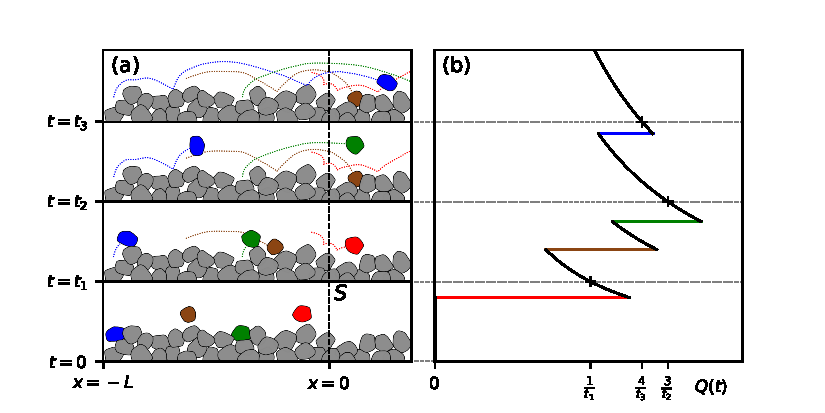
\includegraphics{./figures/ch2/figure1.pdf}}
	\caption{The left panel indicates the configuration for the flux. The particle trajectories within are calculated from equation \ref{eq:langevin}, demonstrating alternation between rest and motion with fluctuating velocity. Particles begin their transport with positions $-L\leq x \leq 0$ at $t=0$, and as depicted in the right panel, the flux is calculated as the number of particles $N_>(t)$ which lie to the right of $x=0$ at the observation time $t$, divided by $t$: $Q(t) = t^{-1}N_>(t)$. We calculate the probability distribution of $Q$ over all realizations of the trajectories and initial positions as $L\rightarrow \infty$}
	\label{fig:fig1}
\end{figure}

The rate of particles crossing the surface in an observation time $T$ is
\be Q(T) = \frac{1}{T}\sum_{i=1}^N \mathcal{I}_i(T). \ee
In this equation, $\mathcal{I}_i(T)$ is an indicator function which is $1$ whenever the $i$th particle has passed our control surface and $0$ otherwise. All particles which have not crossed the control surface (or which have crossed and then crossed back) contribute nothing to the flux. The probability distribution of the flux is then 
\be P(Q|T) = \Big \bra \delta\Big( Q - \frac{1}{T}\sum_{i=1}^N \mathcal{I}_i(T) \Big) \Big\ket. \ee
The average is over the initial conditions of each particle and the ensemble of trajectories for each particle.
Taking the Laplace transform over $Q$ (i.e. forming the characteristic function) obtains
\begin{align} \tilde{P}(s|T) &= \Bigg\bra \int_0^\infty dQ e^{-s Q}\delta\Big( Q - \frac{1}{T}\sum_{i=1}^N \mathcal{I}_i(T) \Big)\Bigg\ket \\
	&=  \Big\bra \exp\Big(\frac{s}{T}\sum_{i=1}^N \mathcal{I}_i(T)\Big)\Big\ket \\
	&=  \prod_{i=1}^N \Big\bra \exp\Big(-\frac{s}{T}\mathcal{I}_i(T)\Big)\Big\ket \\
	&= \prod_{i=1}^N \Big[1-\big(1-e^{-s/T}\big)\big\bra \mathcal{I}_i(T) \big\ket \Big] \end{align}
This progression relies on the independence of averages for each particle (so the average of a product is the product of averages) and the fact that  $ \mathcal{I}_i(T)$ is either $1$ or $0$, so that $e^{ax} = 1-(1-e^a)x$.
The average over initial conditions and possible trajectories for the $i$th particle can be written
\be \bra \mathcal{I}_i(t) \ket = \frac{1}{L}\int_L^0 dx' \int_0^\infty dx \mathcal{P}(x,t|x') =  \frac{1}{L}\int_0^L dx' \int_0^\infty dx \mathcal{P}(x,t|-x'), \ee
where $\mathcal{P}(x,t|x')$ is the probability density that the particle is found at position $x$ at time $t$ given it was initially at $x'$ at time $0$. This is the part of the flux that depends on the particle dynamics (ie instantenous velocities and entrainment/deposition characteristics).

Inserting (7) into (6) and taking the limit as $L\rightarrow \infty$ and $N \rightarrow \infty$ while the density of particles $\rho = N/L$ remains constant provides
\be \tilde{P}(s|T) = \lim_{N \rightarrow \infty} \Big(1 - \frac{1}{N}\big(1-e^{-s/T}\big)\mu(T) \Big)^N = \exp \Big[ -\big(1-e^{-s/T}\big)\mu(T) \Big].\ee
where $\mu(T) = \rho \int_0^\infty dx \int_0^\infty dx' \mathcal{P}(x,T|x')$ is a rate constant which encodes the particle dynamics. This expression is the characteristic function of a Poisson distribution \citep{Cox1965}.
Expanding in $e^{-s/T}$ and inverting the Laplace transform provides the probability distribution of the flux, contingent on the sampling time $T$:
\be P(Q|T) = \sum_{k=0}^\infty \frac{\mu(T)^k}{k!}e^{-\mu(T)}\delta(Q-\frac{k}{T}).\ee
This equation implies that the mean flux is $\bra Q \ket(T) = \int_0^\infty dQ Q P(Q|T) = \mu(T)/T$, and similarly the variance is $\sigma_Q^2(T) = \mu(T)/T^2$. 
The conclusion is that if the flux is considered as a time averaged number of particles crossing a control surface, the mean flux is always Poissonian, no matter how particles move, provided the particles are independent and do not interact.


\section{Results \label{sec:res}}
\subsection{The position probability distribution and its moments}
\begin{figure}
	\centerline{\includegraphics{figures/ch2/figure2_slopeKey.pdf}}
	\caption{Panel (a) indicates the probability distribution of particle position as it evolves through time. From the initial mixture of motion and rest states, particles advect downstream as they diffuse due to differences in their fluctuating velocities and exchange between motion and rest. Panel (b) shows the resulting particle diffusion. At timescales $t \ll 2D/V^2$, the diffusion is normal since the movement is approximately a standard diffusion process (as advection is irrelevant on these timescales). For larger timescales, $2D/V^2 \ll t \ll \tau$, particles undergo ballistic diffusion similar to \citet{Lisle1998} as a result of some particles being stationary as others advect. Finally longer than the timescale $\tau = 1/k$ associated with entrainment and deposition, diffusion is again normal, exemplified by exchange between motion and rest. All results are scaled by the mean hop length $l=V/k_D$ and the autocorrelation time $\tau=1/k$ of the motion/rest alternation.}
	\label{fig:fig1}
\end{figure}
The master equation \ref{eq:master} describes the evolution of the probability distribution of position through time. Loosely speaking the solution of this equation is expected to be some combination of the \citet{Einstein1937} theory for particle transport with the Gaussian propagator of the advection-diffusion equation \citep{Morse1953a}. 

Because the master equation is second order in time, it requires initial conditions for $P$ and $\pt P$. Considering that particles start at rest in a mixture of motion and rest states, with a fraction $k_E/k$ starting in motion and a fraction $k_D/k$ starting in rest, these conditions derive from the state 
\be P(x,0) = \lim_{t\rightarrow 0 } \frac{k_E}{k} \sqrt{\frac{1}{4\pi D t}} \exp\Big[-\frac{(x-Vt)^2}{4Dt}\Big]+ \frac{k_D}{k}\delta(x)\ee
which gives $P(x,0) = \delta(x)$ and $ \pt P(x,0) = \frac{k_E}{k}\big[D\delta''(x)-V \delta'(x) \big]$ \citep{Weiss2002a}.

The master equation \ref{eq:master} is solved by transform calculus in the appendix, providing
\begin{multline} P(x,t) = \big[-\varphi D\px^2 + V\varphi \px + k + \pt \big]\int_0^t \mathcal{I}_0\Big( 2 \sqrt{k_Ek_D u(t-u)}\Big) e^{-k_E(t-u)} \\ \times \sqrt{ \frac{1}{4\pi D u}} \exp\Big[-k_D u - \frac{(x-Vu)^2}{4Du}\Big] du. \label{eq:monster}
 \end{multline}
This integral term encodes the earlier expectation of Einstein model-like behavior mixed with a Gaussian propagator. The integral term convolves the probability that the particle has been in motion for a period $u$ out of a time $t$ with the probability density that a particle has travelled a distance $x$ in time $u$. The prefactor involving partial derivatives can be understood as adapting this distribution to the initial conditions.

The moments of position from this distribution could be calculated by integrating equation \ref{eq:monster}, but this is challenging. Instead, we calculate the governing equation of the moments directly from the master equation \ref{eq:master}. Multipling this equation by $x^l$ and integrating over all $x$ provides
\be \pt^2 m_l -V l \pt m_{l-1} -k_E V l m_{l-1} + k \pt m_l - D l (l-1) \pt m_{l-2} - k_E D l(l-1) m_{l-2} = 0,\ee
where $\bra x^l \ket = m_l$. 
For $l = 1$, this equation generates the mean position $ \bra x \ket(t) = k_E V t/k$, which is unaffected by diffusion (since Gaussian velocity fluctuations are symmetric).
The case $l=2$ provides the second moment, which provides the variance of position
\be \sigma_x^2 = \frac{2k_Ek_DV^2}{k^3}\Big( t + \frac{1}{k}e^{-k t} - \frac{1}{k}\Big) + 2\frac{k_E D}{k}t.\ee
At short times $t\ll k^{-1}$, this becomes
\be \sigma_x^2 \sim \frac{k_E k_D V^2}{k^2} t^2 + \frac{2 k_E D }{k}t,\ee
so it scales as $\sigma_x^2 \sim t^2$ when $t \gg \frac{2Dk}{V^2 k_D}$ and $\sigma_x^2 \sim t$ when $t \ll \frac{2Dk}{V^2 k_D}$.
Similarly at long times $t\gg k^{-1}$, 
\be \sigma_x^2 \sim \frac{2k_Ek_D V^2}{k^3}t,\ee
so we have a non-trivial multi-scale diffusion phenomenon. 
Provided that $2D/V^2 \ll k_D/k^2$, we therefore have
\be \sigma_x^2 \sim 
\begin{cases}
	 t, & t \ll \frac{2Dk}{V^2 k_D}, \\ 
	 t^2, &  \frac{2Dk}{V^2 k_D} \ll t \ll \frac{1}{k}, \\
	 t, & t\gg \frac{1}{k}.
\end{cases}\ee
Note in the physical condition when $k\approx k_D$, the condition for the existence of three ranges becomes $ \Pe \ll 1,$ where
$\Pe = 2 D k_D/V^2.$
The small Peclet limit, when three diffusion ranges are obtained, is characteristic of bedload sediment transport where velocity fluctuations are typically small compared to mean downstream movement velocites. 

\subsection{Calculation of the sediment flux}

From the formalism in section xxxx, the central parameter of the sediment flux distribution is 
\be \mu(t) = \rho \int_0^\infty dx_i \int_0^\infty dx P(x+x_i,t).\ee
This represents the rate of particles crossing $x=0$ at the observation time $T$ given they started somewhere to left of $x=0$ at $T=0$.

It is convenient to calculate this quantity in Laplace space.   
Taking the Laplace transform,
\be \tilde{\mu}(s) = \rho \int_0^\infty dx_i \int_0^\infty dx \tilde{P}(x+x_i,s),\ee
then performing both integrals provides
\be  \tilde{\mu}(s) = -\frac{\phi D}{V R(s+k_E)} + \frac{2D\phi}{VR(1-R)(s+k_E)} + \frac{4D^2(s+k)}{V^3R(1-R)^2(s+k_E)}. \label{eq:laplacefluxrate}\ee
$\mu(t)$ derives as the inverse Laplace transform of this equation. 
This calculation is performed in the appendix, providing
\begin{multline} 
\mu(t) = \int_0^t \mathcal{I}_0\Big(2\sqrt{k_Ek_Du(t-u)}\Big)e^{-k_E(t-u)-k_D u} \\
\times \Bigg[\sqrt{\frac{D}{\pi u}}\Big([\cev{\partial_t} + k]u-\frac{k_D}{2 k}\Big)e^{-V^2 u/4D} + \frac{V}{2}\Big([\cev{\partial_t} + k]u -\frac{k_D}{k}\Big) \erfc\Bigg(-\sqrt{\frac{V^2 u}{4D}}\Bigg)\Bigg] du. \label{eq:fluxy}
\end{multline}
In this equation, the notation $\cev{\partial}$ means that the derivative acts from the left of all terms in which it is involved, as in $f(t)\cev{partial}_t g(t) = \partial_t f(t)g(t).$

This is a complicated result for the rate constant in the sediment flux \ref{eq:fluxdist}, but this complexity is not surprising given that equation \ref{eq:langevin} involves two interacting diffusion processes. As displayed in \ref{fig:fig3}, as a result of eq. \ref{eq:fluxy} the mean flux takes on a non-trivial scale-dependence, characterized by a decay toward the Einstein prediction $Q_0 = E l$ as the observation time becomes much larger than $1/(k_D \Pe)$. 

\begin{figure}[!htbp]
	\includegraphics[width=\linewidth,keepaspectratio]{figures/ch2/figure3_slopeKey.pdf}
	\caption{}
	\label{fig:fluxconvergence}
\end{figure}
The convergence time of the flux thus scales with the inverse Peclet number. When particle velocity fluctuations during motions are larger compared to advection, the flux becomes slow to converge, in general. 

\subsection{Reduction to earlier work}

The mathematical form of our results is complicated, although the ideas are conceptually clear. Particles alternate through motion and rest, and particle motions have a fluctuating velocity, not a deterministic velocity. 
Nevertheless, turning off velocity fluctuations by setting $D=0$ re-derives the results of \citet{Lisle1998}, who formulated sediment transport as a random walk between motion and rest states.
Further taking the velocity infinite as the time spent in motion vanishes, while their product $V/k_D = \ell$, the mean step distance, rederives the central result of \citet{Einstein1937}, given originally in \ref{eq:einsteinpdf}.

In either of these limit cases, the mean sediment flux becomes $\bra q \ket = E \ell$, with no dependence on observation scale. This indicates that scale dependence in the sediment flux is a consequence of velocity fluctuations among moving particles, at least when observation timescales are relatively short.
 
\section{Discussion \label{sec:disc}}

This chapter has generalized the earlier descriptions of individual sediment trajectories \citep[e.g.][]{Lisle1998,Lajeunesse2017} to include velocity fluctuations in the motion state. Using results from this generalized model as an example, I demonstrated how to calculate the sediment flux probability distribution, phrasing earlier renewal theory approaches more directly in terms of the underlying particle dynamics \citep[e.g.][]{Turowski2010,Ancey2020}. 
Calculated in this way, the sediment flux distribution is observation-scale dependent, describing how sediment fluxes depend on the period over which they are measured.

\subsection{Fluctuations and collective motions}

The sediment flux probability distribution in equation \ref{eq:fluxdist} represents a Poisson distribution with an observation-scale dependent rate.
Poisson distributions have a relatively thin tail, meaning fluctuations are typically small \citep{Ancey2006}.
In reality, sediment flux distributions are only Poissonian at high transport rates, whereas in other conditions they have wide tails representing the possibility of extremely large transport fluctuations \citep{Ancey2008,Turowski2010,Dhont2018,Saletti2015} which appear as bursts \citep[e.g.][]{Goh2008} in the sediment flux timeseries \citep{Singh2009, Heyman2013,Benavides2021}. This exposes a need to generalize a mechanistic theory of the sediment flux I developed here to produce wider fluctuations.

Descriptions of sediment transport based on population dynamics in a control volume have realistically-wide fluctuations by incorporating a positive feedback between the number of moving particles and the particle entrainment rate called collective entrainment \citep{Ancey2008,Ancey2014}.
This feedback generates spatially-correlated waves of moving particles \citep{Ancey2014, Heyman2015} and produces non-exponential interarrival time distributions \citep{Heyman2013} which imply wide-tailed flux distributions when incorporated in renewal theory \citep{Turowski2010,Ancey2020}.
Collective entrainment has been attributed to particle-particle interactions, such as small granular avalanches and collision-induced entrainment, and to fluid-particle interactions, such as large eddies entraining particles as they sweep downstream \citep{Heyman2014a,Ancey2014,Lee2018}.

We can imagine generalizing the description in equation \ref{eq:flipfloplangevin} to include such fluid-particle interactions by including time dependence in the movement velocity ($V$), diffusivity ($D$), or entrainment and deposition rates ($k_E$ and $k_D$) as necessary, although the resulting equations would likely require numerical solutions.
Particle-particle interactions would be more challenging to include.
The dynamical equation \ref{eq:flipfloplangevin} would generalize to $\dot{x}_i(t) = F_i(x_i,t) + \sum_{i\neq j}G_{ij}(\{x_j\},t)$, where the $F_i$ are the driving terms unique to each particle, while the $G_{ij}$ are some (generally stochastic) terms representing interactions between the $i$th and $j$th particles \citep{Goldstein1997}. The resulting joint distribution of particle positions and velocities ($P(x_1,v_1,\dots,x_{N(t)},v_{N(t)},t)$) might be formulated by analogy to the theory of reaction diffusion systems \citep{Pechenik1999, Cardy2008}, non-ideal gases \citep{Chapman1970,Brilliantov2004}, or other interacting particle models available in physics literature \citep{Hernandez2004,Escaff2018}. 
By analogy to collective entrainment, interacting models which generalize the approach established in this chapter should be capable of producing wide sediment transport fluctuations.

\subsection{Measurement protocol for the sediment flux}




\subsection{Stochasticity in landscape evolution}

\citet{Exner1925} originally phrased channel morphodynamics in terms of spatial gradients in the sediment flux (sec. \ref{sec:landscape}), writing
\be (1-\phi) \pt h(x,t) = -\px q(x,t). \ref{eq:stocEx}\ee
In this one-dimensional equation, $h(x,t)$ is a continuous field representing the longitudinal channel profile.
Traditionally, the Exner equation is evaluated considering the flux as a deterministic quantity \citep{Parker2007,Viparelli2011,An2017}, which provides a solitary trajectory of the profile through time.

Considering the flux in the Exner equation as a stochastic quantity requires us to reinterpret channel dynamics in a way which few researchers have explored \citep{Jerolmack2005,Bohorquez2016}.
In contrast to the traditional analysis, a stochastic Exner equation with fluctuating $q(x,t)$ generates an ensemble of possibilities for the channel profile $z(x)$ at each instant. This set of possibilities is characterized by a probability distribution $P(\{z(x)\},t)$ for each possible profile.
Mathematically, since the channel profile is a field, evaluating such a probability distribution of channel profiles would require statistical field theory \citep{Kardar2007}.
A starting point on this analysis might be $P(\{z(x)\},t) = \bra \delta[z(x,t)-h(x,t)]\ket,$ where $h(x,t)$ involves the stochastic flux $q(x,t)$ from equation \ref{eq:stocEx}.
In this equation, $\delta[f(x)]$ is a Dirac delta functional, which generalizes the delta function $\delta(x)$ from a single-valued parameter $x$ to a continuous field $f(x)$.
Such ideas are commonly applied to understand polymers and membranes \citep{Kawakatsu2001,Nelson2004}, but they have not been introduced in geomorphology.

Introducing such a description with the stochastic Exner equation would lend new mathematical language to the old unsolved problem in geomorphology: how does variability affect landscape evolution?

\section{Summary and Conclusion \label{sec:conc}} 
 
This chapter introduced a two-noise stochastic dynamical equation to describe individual bedload trajectories for particles alternating between motions and rests. The motion phase was enriched to include velocity fluctuations, forming the first physical model of this type.
The probability distribution of the bedload sediment flux was calculated from these particle dynamics, and the resulting flux distribution was demonstrated to adopt scale-dependence from the underlying trajectories of individual particles. The measurement timescales over which sediment flux observations converge were expressed in terms of the mean particle movement velocity and the typical magnitude of its fluctuations in terms of a Peclet number.
 
These results generalize the bedload trajectory models of \citet{Einstein1937}, \citet{Lisle1998}, and \citet{Lajeunesse2017} to include fluctuating movement velocities, and they reframe earlier renewal models of the sediment flux probability distribution \citep{Lajeunesse2010,Ancey2020} to explicitly include the transport dynamics of individual sediment grains. They further quantify the dependence of the sediment flux on the observation scale, and provide guidance as to the measurement times required to resolve sediment transport without ambiguity, at least in simplified configurations when bedforms are absent. 
Next steps are to include interactions between particles to produce wider sediment transport fluctuations, and to evaluate the effects of sediment transport fluctuations on channel morphodynamics.




%%%%%%%%%%%%%%%%%%%%%%%%%%%%%%%%%%%%%%%%%%%%%%%%%%%%%%%%%%%%%%%%%%%%%%%%%%%%%%%%%%%%%%%%%%%%%%%%%%%%%%%%%%%%%%%%%%%%%%%%%%%%%%%%
%%%%%%%%%%%%%%%%%%%%%%%%%%%%%%%%%%%%%%%%%%%%%%%%%%%%%%%%%%%%%%%%%%%%%%%%%%%%%%%%%%%%%%%%%%%%%%%%%%%%%%%%%%%%%%%%%%%%%%%%%%%%%%%%
%%%%%%%%%%%%%%%%%%%%%%%%%%%%%%%%%%%%%%%%%%%%%%%%%%%%%%%%%%%%%%%%%%%%%%%%%%%%%%%%%%%%%%%%%%%%%%%%%%%%%%%%%%%%%%%%%%%%%%%%%%%%%%%%
%%%%%%%%%%%%%%%%%%%%%%%%%%%%%%%%%%%%%%%%%%%%%%%%%%%%%%%%%%%%%%%%%%%%%%%%%%%%%%%%%%%%%%%%%%%%%%%%%%%%%%%%%%%%%%%%%%%%%%%%%%%%%%%%
\endinput
Introducing such a description with the stochastic Exner equation would lend new mathematical language to the old unsolved problem in geomorphology: how does variability affect landscape evolution?
The classic works all acknowledge variability \citep{Leopold1952}, although one of their main efforts was to construct strategies to describe landscapes without explicitly accounting for it, producing ideas like competent flows to summarize climatic variability \citep{Wolman1960}, characteristic grain sizes to overcome sorting processes \citep{Parker1982}, or average flow energies to avoid turbulence \citep{Bagnold1954}.
Progress in stochastic approaches to river science \citep[e.g.][]{Furbish2021c,Ancey2020b} invites us to step beyond averaged descriptions, propagate noises through the governing equations of landscape evolution, and ask again with these classic works to what extent fluctuations shape Earth's surface.


This chapter upscaled from individual particle motions to calculate the sediment flux.
We can imagine going further, to upscale from the sediment flux to understand channel morphodynamics.
The sediment flux is stochastic as a result of variability in the individual particle trajectories forming it.
As a result, the channel morphodynamics should also adopt this stochasticity, although very few studies have evaluated this possibility \citep{Bohorquez2016, Jerolmack2005}.




Earlier approaches to calculate the probability distribution of the sediment flux have counted the fluctuating number of particles in a control volume with population models \citep{Ancey2008,Ancey2014}, or they have evaluated the average rate of particles crossing a control surface using the interarrival time distribution of particles from upstream \citep{Turowski2010,Ancey2020,Heyman2013}, in what is basically an application of renewal theory \citep{Cox1962}.
These approaches can be described as ``kinematic", in that they do not explicitly account for the trajectories of individual particles as they move downstream.

Here, I have demonstrated how to describe the sediment flux probability distribution from a dynamical perspective, rather than a kinematic one, using stochastic dynamical equations to describe the downstream trajectories of individual grains (eq. \ref{eq:langevin}.
In effect, the interarrival time distribution is replaced by the probability distributions of position for all individual particles available for motion, with their initial positions and velocities considered as random variables.
Particles moving downstream are counted as they cross the control surface, giving rise to a parameter $\Lambda(T)$, dependent on observation scale, which is analogous to the heuristic rate constant in the renewal theories that were reviewed in section \ref{sec:renewal} \citep{Turowski2010,Ancey2020}
This new description of the sediment flux from the grain scale particle dynamics, rather than characteristic kinematics derived from them, represents considerable progress toward a mechanistic understanding of sediment transport from statistical physics.

\subsection{Outlook and future research}

The phrasing of sediment fluxes the topographies they moderate as statistical quantities, having mean configurations and fluctuations, provides some context on the severe challenges encountered in predicting landscape change with deterministic equations \citep{}.
What we observe, looking at Earth's landscapes, may be a single realization, drawn from a spectrum of possibilities, whose precise form evades description. 
The stochastic perspective allows us to 

The sediment flux probability distribution in equation \ref{eq:fluxdist} represents a Poisson distribution with an observation-scale dependent rate.
Poisson distributions have a relatively thin tail, meaning fluctuations are typically small \citep{Ancey2006}. This contrasts with many bedload transport experiments with wide-tailed fluctuations \citep{Ancey2008,Heyman2016,Fathel2015}, especially for weak flow conditions near initiation of particle motion \citep{Benavides2021}, exposing a need to generalize a mechanistic theory of the sediment flux developed here to provide wider fluctuations.

There are essentially two mechanisms available by which wide fluctuations can arise \citep{Goh2008}. Both would be ultimately reflected in non-exponential interarrival times of particles \citep[e.g.][]{Turowski2010,Heyman2013}, although their origins would be unambigiously linked to the underlying particle transport mechanics.
The first possibility is to introduce correlations between particle movements \citep{Ancey2008,Heyman2013,Ancey2014}, such as might arise when turbulent flow fluctuations entrain many particles at once \citep{Cameron2020} or drive waves of high velocity particles downstream simultaneously \citep{Nino1996}. 
In a theory such as the one I presented here, this first mechanism for wide fluctuations could be described by temporally unsteady velocities, entrainment or deposition rates, or diffusion coefficients in the Langevin model \ref{eq:langevin}.
The second possibilty is to introduce interactions between moving particles, such as might result from collisions \citep{Lee2018} or wake vortices \citep{Schmeeckle2014} inducing particle entrainment, leading to collective waves of motion \citep{Ancey2014}.
Including such effects would require a many-body generalization of the Langevin and master equations \ref{eq:langevin} and \ref{eq:master}, where the probability distribution of position is promoted to a joint form $P(x_1,v_1,\dots,x_{N(t)},v_{N(t)},t)$, which is puzzling, since the number of particles $N(t)$ in the distribution fluctuates.
The model of \citet{Ancey2014} hints at this possibility, although its starting point is not a dynamical equation as in \ref{eq:master}.
Some hints as to how to generalize our work to include interactions between particles to describe wide-tailed sediment fluxes can be gleaned from literature on reaction-diffusion processes \citep{Hernandez2004,Cardy2006} and interacting gases \citep{Chapman1970,Brilliantov2004}. The further inclusion of interacting particle models into bedload transport theory would be an exciting development.


%%!TEX root = diss.tex

\chapter{Analysis of bed elevation change and sediment transport fluctuations}
\label{ch:ch3}

The transport characteristics of coarse grains moving under a turbulent flow ultimately control a wide set processes within rivers, including the export of contaminants \citep{Malmon2005,Macklin2006}, the success of ecological restoration efforts \citep{Gaeuman2017}, and the response of channel morphology to disturbances \citep{Hassan2017}.
Although the displacements of individual grains are a mechanical consequence of forces imparted from the flow, bed, and other grains \citep{Wiberg1985, Vowinckel2014,Gonzalez2017}, accurately characterizing these forces within natural channels is practically impossible, especially considering the intense variability these forces display \citep{Schmeeckle2007,Celik2010, Dwivedi2011}.
In response, researchers have developed a stochastic concepts of bedload transport \citep{Einstein1937}, whereby the erosion and deposition of individual grains are modeled as the random results of undetermined forces \citep{Einstein1950,Paintal1971,Ancey2006}.

Essentially two types of bedload transport model have been developed from this concept.
The first type provides the probabilistic dynamics of a small population of tracer grains as they transport downstream \citep{Einstein1937,Hubbell1964, Nakagawa1976,Martin2012,Lajeunesse2017,Wu2019}, while the second provides the statistics of the number of moving grains (``the particle activity'') within a control volume \citep{Einstein1950,Ancey2006,Furbish2012a}.
In the first type, individual displacements are considered to result from alternate step-rest sequences, where step lengths and resting times are random variables following statistical distributions \citep{Einstein1937}. 
Differences between the random-walk motions of one grain and the next imply a spreading apart (i.e., diffusion) of tracer grains as they transport downstream.

Resting time distributions have been carefully studied in relation to these models because the predicted diffusion characteristics are critically dependent on whether the distribution has a light or heavy tail \citep{Bradley2017,Martin2012,Weeks1998}.
Resting times have puzzled researchers because early experiments showed exponential distributions \citep{Einstein1937,Hubbell1964, Yano1969,Yano1969a,Nakagawa1976}, while later experiments showed heavy-tailed power-law distributions \citep{Martin2012,Voepel2013, Olinde2015, Pretzlav2016a, Bradley2017, Liu2019}.
A predominant hypothesis is that power-law distributed resting times originate from buried grains \citep{Martin2014,Voepel2013}. This permits surface grains to retain exponential resting times. 
Conceptually, when grains rest on the surface, material transported from upstream can deposit on top of them, preventing entrainment until its removal, driving up resting times and imparting a heavy tail to the distribution.

\citet{Martin2014} have provided the only direct support for this hypothesis by tracking grains through complete cycles of burial and exhumation in a narrow flume.
They observed heavy-tailed resting times of buried grains and described their results with a mathematical model similar to an earlier effort by \citet{Voepel2013}.
Both of these models treat bed elevation changes as a random walk and interpret resting times as return periods from above in the bed elevation timeseries \citep{Redner2007}.
Each describes resting time distributions from different experiments, but they rely on different random walk models, and their treatment of bed elevations as a process independent of sediment transport is questionable at first glance, since bedload transport is the source of bed elevation changes \citep{Wong2007}, yet neither model explicitly describes bedload transport.
Models of sedimentary bed evolution incorporating sediment transport processes might enhance understanding of sediment resting times.

The second type of stochastic model prescribes rates (probabilities per unit time) to the erosion and deposition events of individual grains within a control volume to calculate the particle activity \citep{Einstein1950}.
These approaches aim at a complete statistical characterization of the bedload flux \citep{Furbish2012a,Fathel2015,Furbish2017,Heyman2016}, including probability distributions \citep{Ancey2006,Ancey2008}, spatial and temporal characteristics of its fluctuations \citep{Heyman2014a, Roseberry2012,Dhont2018}, and the dependence of these statistical characteristics on the length and timescales over which they are observed \citep{Singh2009,Singh2012,Saletti2015}.
A recent surge in research activity has generated rapid progress in this subject. 
For example, \citet{Ancey2006} demonstrated that a constant erosion rate as originally proposed by \citet{Einstein1950} was insufficient to develop realistically large particle activity fluctuations, so they added a positive feedback between the particle activity and erosion rate they called ``collective entrainment'' \citep{Ancey2008, Heyman2013,Heyman2014, Lee2018}.
While this feedback was deemed necessary to model realistic activity fluctuations, the implications of collective entrainment for the bed topography have not been fully explored.

In this work, I present the first stochastic model coupling the erosion and deposition of individual bedload grains to local bed elevation changes.
This model extends the birth-death model approach reviewed in Sec. \ref{sec:birthdeath} to describe the interplay between the bedload flux and the bed elevation within a control volume.
This new model evaluates the effect of collective entrainment on bed elevation change, and it allows for investigations of the residence times of particles buried under the bed surface.
The model has two major assumptions: First, bedload erosion and deposition are characterized by probabilities per unit time, or rates \citep{Einstein1950, Ancey2008}; and second, these rates are contingent on the local bed elevation, encoding the property that erosion of sediment is emphasized from regions of exposure, while deposition is emphasized in regions of shelter \citep{Sawai1987, Wong2007}.

Below, Sec. \ref{sec:elemodel} introduces the stochastic model and Sec. \ref{sec:elesolution} solves it with a mixture of numerical and analytical techniques. Model solutions illustrate several new features of particle activity and bed elevation statistics that result from feedbacks between the erosion and deposition rates with bed elevation change. Sec. \ref{sec:eleresults} present these features, while Secs. \ref{sec:elediscussion} and \ref{sec:eleconclusion} conclude with the implications of these features and the suggestions they raise for future research.

\section{Stochastic model of bedload transport and bed elevations}
\label{sec:elemodel}

The model in this chapter is formulated by considering a volume of downstream length $L$ containing some number $n$ of moving particles in the flow and some number $m$ of stationary particles composing the bed at time $t$, as depicted in Fig. \ref{fig:eledefinition}. The value $m$ is defined relative to the mean number of grains within the control volume, so that it can be either positive or negative. $n$ is always a positive integer including $0$.

All particles are considered approximately spherical with the same radius $a$, so their mobility and packing characteristics are similar from one particle to the next.
Following \citet{Ancey2008}, basically four events can occur at any instant to modify the populations $n$ and $m$.
These events are (1) migration of a moving particle into the volume from upstream ($n \rightarrow n+1$), (2) the entrainment (erosion) of a stationary particle into motion within the volume ($m\rightarrow m-1$ and $n\rightarrow n+1$), (3) the deposition of a moving particle to rest within the volume ($m\rightarrow m+1$ and $n\rightarrow n-1$), and (4) the migration of a moving particle out of the volume to downstream ($n\rightarrow n-1$).
The four events are depicted as arrows in Fig. \ref{fig:eledefinition}.
As the events occur at random intervals, they set up a joint stochastic evolution of the populations $n$ and $m$ characterized by a joint probability distribution $P(n,m,t)$ for the number of particles in motion and rest in the volume at $t$.
\begin{figure}[!htbp]
	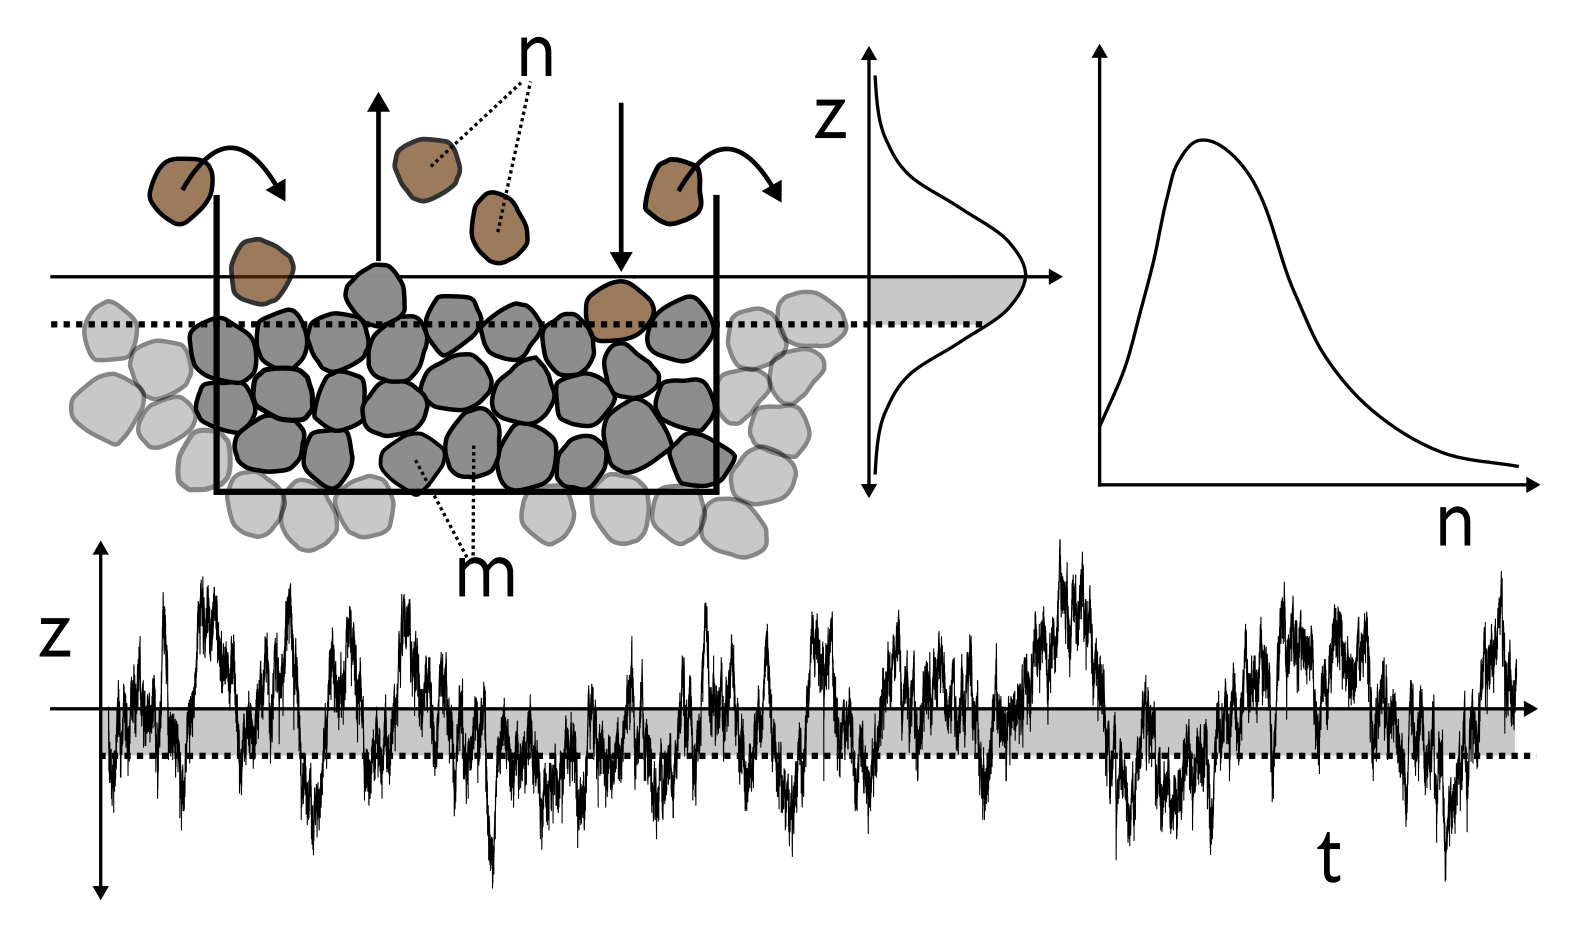
\includegraphics[width=\linewidth,keepaspectratio]{./figures/ch3/improveddef.png}
	\caption{Definition sketch of a control volume containing $n$ moving grains and $m$ resting grains. Migration, entrainment, and deposition are represented by arrows, and the instantaneous bed elevation is depicted by dotted lines. The bed is displayed in a degraded state, where $m<0$. The marginal distributions of $n$ and $m$ are indicated in the upper right, while the bottom panel is a realized timeseries of bed elevations computed from $m$ using Eq. \ref{eq:ele}.}
	\label{fig:eledefinition}
\end{figure}

The populations $n$ and $m$ provide the volumetric bedload flux $\Phi$ and the local bed elevation $z$.
The mean transport rate is given by $\Phi = u_s\langle n \rangle/L$, where $u_s$ is the characteristic velocity of moving bedload and $\langle n \rangle = 
\sum_{n,m}nP(n,m) $ is the mean number of grains in motion \citep{Charru2004, Ancey2008, Furbish2012a}.
The bed elevation is related to $m$ through the packing geometry of the bed.
This relationship depends on the packing fraction $\phi$ of grains in the bed \citep{Bennett1972}. Considering the bed as two-dimensional \citep{Einstein1950, Paintal1971}, the deviation from the mean bed elevation can be expressed as
\begin{equation} z(m) = \frac{\pi a^2}{\phi L}m = z_1 m. \label{eq:ele}\end{equation}
The constant $z_1 = \pi a^2/(\phi L)$ is an important scale in the problem. 
$z_1$ is the magnitude of bed elevation change in an average sense across the control volume associated with the addition or removal of a single grain.

Bed elevation changes modify the likelihood of entrainment and deposition in a negative feedback \citep{Sawai1987, Wong2007}. Aggradation increases the likelihood of entrainment, while degradation increases the likelihood of deposition.
\citet{Wong2007} concluded that bed elevation changes induce an exponential variation in entrainment and deposition probabilities, while \citet{Sawai1987} concluded that the variation is linear.
For simplicity, this chapter utilizes the scaling of \citet{Sawai1987}. This scaling is equivalent to the  \citet{Wong2007} scaling when bed elevation changes are small.
Because experimental distributions of bed elevations are often symmetrical \citep[e.g.][]{Crickmore1962, Pender2001,Wong2007, Martin2014}, the erosion and deposition feedbacks are considered to have the same strength.
As bed elevation changes drive up (down) erosion rates, so they drive down (up) deposition rates to the same degree.

Merging these ideas with those of \citet{Ancey2008} produces expressions for the four possible transitions with local bed elevation-dependent entrainment and deposition rates:
\begin{align}
	&R_{MI}(n+1|n) = \nu && &\text{migration in}, \label{eq:rate1}\\
	&R_E(n+1,m-1|n,m)=(\lambda + \mu n)[1 + \kappa m], && &\text{entrainment}, \label{eq:rate2}\\
	&R_D(n-1,m+1|n,m)=\sigma n [1- \kappa m ], && &\text{deposition}. \label{eq:rate3} \\
	&R_{MO}(n-1|n) =\gamma n && &\text{migration out} \label{eq:rate4}.
\end{align}
In Eqs. \ref{eq:rate2} and \ref{eq:rate3}, $\kappa$ is a coupling constant between bed elevations and the entrainment and deposition rates.
Using this coupling constant, I will later demonstrate the relationship
\begin{equation}\kappa \approx \big(\frac{z_1}{2l}\big)^2 \label{eq:active}
\end{equation}
where $l$ is a characteristic length scale of bed elevation change that can be interpreted as the active layer depth \citep{Wong2007,Church2017}.
$\nu$ is the rate of migration into the control volume, $\lambda$ is the conventional entrainment rate, $\mu$ is the collective entrainment rate, $\sigma$ is the deposition rate, and $\gamma$ is the rate of migration out of the control volume.
At $m=0$, these equations reduce to those of the \citet{Ancey2008} model.
Away from this elevation, entrainment and deposition are alternatively suppressed or enhanced depending on the sign of $m$, constituting a feedback between bed elevations and entrainment and deposition.

All four rates are independent of the past history of the populations and depend only on the current populations $(n,m)$. 
As a result, the model is Markovian \citep{Cox1965, VanKampen2007}, meaning time intervals between any two subsequent transitions are exponentially distributed \citep{Gillespie2007}.

The master equation for the probability flow can be written using the Komogorov equation
 $\partial P(n,m;t)/\partial t = 
\sum_{n',m'} [R(n,m|n',m')P(n',m';t)-R(n',m'|n,m)P(n,m;t)]$ \citep{Cox1965, Gillespie1991, Ancey2008} as 
\begin{multline}
	\frac{\partial P}{\partial t}(n,m;t) =  
	\nu P(n-1,m;t) + [\lambda(m+1) + \mu(n-1)][1+\kappa(m+1)]P(n-1,m+1;t)\\  
	+ \sigma(n+1)[1-\kappa(m-1)]P(n+1,m-1;t) + \gamma(n+1) P(n+1,m;t) \\
	- 
	\{ \nu + \lambda+ \mu n (1+\kappa m) +  \sigma n ( 1- \kappa m) + \gamma n \}P(n,m;t).
	\label{eq:elemaster}
\end{multline}
The joint distribution $P(n,m;t)$ that solves this equation fully characterizes the statistics of $n$ and $m$ -- proxies for the bedload flux and local bed elevation.

The average entrainment and deposition rates $E$ and $D$ over all bed elevations are $E = \lambda +\mu \langle n \rangle$ and $D=\sigma \langle n \rangle$.
The solutions of Eq. \ref{eq:elemaster} should be expected to adjust from whatever initial conditions toward a steady-state distribution $P_s(n,m)$ -- independent of time -- if the constant factors in the transition rates are representative of equilibrium transport conditions.
Equilibrium requires $E=D$, meaning there is no net change in elevation, and $\nu = \gamma \langle n \rangle$, meaning mass is conserved in the control volume (inflow $=$ outflow).
This master equation describes a two-species stochastic birth-death model \citep{Cox1965} of a type well-known in population ecology \citep{Pielou1977, Swift2002} and chemical physics \citep{Gardiner1983}.
In context of this chapter, the two populations are the moving and stationary grains in the control volume.

\section{Model solutions}
\label{sec:elesolution}

Unfortunately, Eq. \ref{eq:elemaster} does not admit an analytical solution unless $\kappa=0$ (but see \citet{Swift2002} for the generating function method which fails in this case).
The difficulty originates from the product terms between $n$ and $m$ representing the bed elevation dependence of collective entrainment and deposition rates.

Because the model is Markovian, it is nevertheless possible to numerically simulate Eq. \ref{eq:elemaster} with the Gillespie algorithm \citep{Gillespie1977, Gillespie1991, Gillespie2007}. 
In conditions when the coupling constant $\kappa$ between the entrainment/deposition rates and the bed elevation is weak, it is also possible to solve the master equation approximately with mean field and Fokker-Planck approaches \citep{Haken1978,Gardiner1983}.
The Gillespie simulation algorithm is described below in Sec. \ref{sec:elenumerical}, while these analytical approximations are described in Sec. \ref{sec:eleanalytical}.

\subsection{Numerical study of the joint model}
\label{sec:elenumerical}

The Gillespie algorithm takes advantage of the defining property of a Markov process: when transition rates are independent of history, time intervals between transitions are
exponentially distributed \citep{Cox1965}.

As a result, to step the Markov process through a single transition, one can draw a first random value from the exponential distribution of transition intervals to determine the time of the next transition,
then draw a second random value to choose the type of transition that occurs using relative probabilities formed from Eqs. \ref{eq:rate1} - \ref{eq:rate4}. The transition is enacted by shifting $t$, $n$, and $m$ by the appropriate values to the type of transition (that is, entrainment is $m\rightarrow m-1$ and $n \rightarrow n+1$, and so on).
This procedure can be iterated to form an exact realization of the stochastic process \citep{Gillespie2007}.
The appendix Secs. \ref{sec:arr}-\ref{sec:crr} provide additional background on the stochastic simulation method.

Using this method, I simulated 4 transport conditions with 13 different values of $l$ taken across a range from $l=a$ (a single radius) to $l=10a$ (10 radii).
These values include the range exhibited by the available experimental data on bed elevation timeseries \citep{Wong2007,Singh2009,Martin2014}.

\begin{wraptable}{r}{0.6\textwidth}
	\caption{Migration, entrainment, and deposition rates at $z(m)=0$ from \citet{Ancey2008}. Units are $s^{-1}$ (probability/time). Bed elevation changes modulate these rates in accord with Eqs. \ref{eq:rate1}-\ref{eq:rate4}.}\label{tab:anceyparams}
	\begin{tabular}{cccccc} \\ 
		\toprule  
		flow & $\nu$ & $\lambda$ & $\mu$ & $\sigma$ & $\gamma$ \\
		\midrule
		(a) & 5.45  & 6.59  & 3.74 & 4.67 & 0.77 \\
		\midrule
		(g) & 7.74  & 8.42  & 4.34 & 4.95 & 0.56 \\
		\midrule
		(i) & 15.56 & 22.07 & 3.56 & 4.52 & 0.68 \\
		\midrule
		(l) & 15.52 & 14.64 & 4.32 & 4.77 & 0.48 \\
		\bottomrule
	\end{tabular}
\end{wraptable}
For the migration, entrainment, and deposition parameters representing bedload transport at each flow condition $(\nu, \lambda, \mu, \sigma, \gamma)$, I used the values measured by \citet{Ancey2008} in a series of flume experiments: these are summarized in table \ref{tab:anceyparams}.
Flow conditions are labeled (a), (g), (i), and (l), roughly in order of increasing bedload flux (see \citet{Ancey2008} for more details). 
In all simulations, I took the packing fraction $\phi = 0.6$ -- a typical value for a pile of spheres \citep[e.g.][]{Bennett1972}, and I set $L = 22.5$cm and $a = 0.3$cm, values from the original \citet{Ancey2008} experiments.
Each simulation was run for $250$ hours of virtual time, a period selected to ensure convergence of particle activity and bed elevation statistics.

\subsection{Approximate solutions of the joint model}
\label{sec:eleanalytical}

The $n$ and $m$ dynamics in Eq. \ref{eq:elemaster} can be approximately decoupled using the inequality $l \gg z_1$ (equivalently $\kappa \ll 1$) which holds for large values of the active layer depth $l$.
These inequalities imply that many entrainment or deposition events are required for an appreciable change in the entrainment or deposition rates.
Concentrating on steady-state conditions $\partial P/\partial t = 0$, one can introduce the exact decomposition $P(n,m) = A(n|m)M(m)$ to Eq. \ref{eq:elemaster}, with the new distributions normalized as $\sum_m M(m)=1$ and $\sum_n A(n|m)=1$ \citep[e.g.][]{Haken1978}.
This provides the steady-state equation
\begin{multline}
	0 =  
	\nu A(n-1|m)M(m) + [\lambda + \mu(n-1)][1+\kappa(m+1)]A(n-1|m+1)M(m+1)\\  
	+ \sigma(n+1)[1-\kappa(m-1)]A(n+1,m-1)M(m-1) + \gamma(n+1)A(n+1|m)M(m) \\
	- 
	\{ \nu + [\lambda+ \mu n ](1+\kappa m) +  \sigma n ( 1- \kappa m) + \gamma n \}A(n,m)M(m).
	\label{eq:decomp}
\end{multline}
Summing this equation over $n$ provides a still exact description of the distribution of bed elevations $M(m)$ in terms of the conditional mean particle activity $\langle n | m \rangle = \sum_{n}nA(n|m)$:
\begin{multline}
	0 =  [\lambda + \mu\langle n | m+1\rangle][1+\kappa(m+1)]M(m+1)
	\\+ \sigma\langle n | m-1\rangle[1-\kappa(m-1)]M(m-1) \\
	- 
	\{  [\lambda+ \mu \langle n | m\rangle ](1+\kappa m) +  \sigma  \langle n | m\rangle( 1- \kappa m) \}M(m).
	\label{eq:approxele}
\end{multline}
Unfortunately, these two equations are no easier to solve than the original master equation, since the amount of coupling between $n$ and $m$ is not reduced in Eq. \ref{eq:decomp}.

The simplest approximation to these equations holds that $\kappa$ is so small that the dynamics of $n$ are totally independent of $m$: $A(n|m) = A(n)$. Taking this limit in Eq. \ref{eq:decomp}, summing over $m$, and using $\langle m \rangle = 0$ reproduces the \citet{Ancey2008} particle activity model.
As shown in Sec. \ref{sec:birthdeath}, this has the solution
\begin{equation} A(n) = \frac{\Gamma(r+n)}{\Gamma(r)n!}p^r(1-p)^n.\label{eq:ancey}\end{equation}
which is a negative binomial distribution for the particle activity with parameters $r=(\nu+\lambda)/\mu$ and $p=1-\mu/(\sigma+\gamma).$
This result implies $\langle n | m \rangle = \langle n \rangle$, so with the definitions of $E$ and $D$ and the equilibrium condition $E=D$, Eq. \ref{eq:approxele} provides
\begin{equation}0 \approx [1+\kappa(m+1)]M(m+1) + [1-\kappa(m-1)]M(m-1)-2M(m). \label{eq:ou} \end{equation}
This mean field equation matches the discrete Ornstein-Uhlenbeck model of bed elevation changes developed by \citet{Martin2014}.
The independent bed elevation and particle activity models of \citet{Martin2014} and \citet{Ancey2008} derive from the model Eq. \ref{eq:elemaster} in a mean field approximation when $\kappa$ is insignificant.

In the appendix Sec. \ref{sec:drr} I show that the Fokker-Planck approximation \citep{Gardiner1983} formed by expanding $M(m\pm 1)$ to second order in $m$ within Eq. \ref{eq:ou} provides the solution $M(m) \propto \exp(-\kappa m^2)$: this is a normal distribution of bed elevations with variance $\sigma_m^2 \propto \frac{1}{2\kappa}$.
As I will demonstrate in Sec. \ref{sec:eleresults}, and as I have already suggested with Eq. (\ref{eq:active}), this is a poor approximation to the bed elevation variance. Nevertheless, this approximation does capture the Gaussian shape of the bed elevation distribution.
The essential issue with this mean field approach is that in actuality, the conditional mean particle activity $\langle n | m \rangle$ varies significantly with $m$, especially when collective entrainment contributes to the mean entrainment rate $E$.

A more careful approximate solution to Eq. \ref{eq:approxele} can be obtained by prescribing a phenomenological equation for $\langle n | m \rangle$ into Eq. \ref{eq:approxele} in order to close the equation for $m$ without solving Eq. \ref{eq:decomp}.
As explained in appendix Sec. \ref{sec:err}, comparison with the numerical simulations determines that
\begin{equation}
	\langle n | m  \rangle \approx \langle n \rangle \Big( 1 - \frac{2\kappa m}{1-\mu/\sigma}\Big) \label{eq:closure}
\end{equation}
captures the general features of the conditional mean particle activity.
Introducing this closure relation to Eq. \ref{eq:approxele}, making the Fokker-Planck approximation, and neglecting terms of $O(\kappa^2)$ provides 
\begin{equation} M(m) \approx M_0 e^{-2\kappa m^2}, \label{eq:ou2}\end{equation}
representing a Gaussian distribution with variance $\sigma_m^2 = \frac{1}{4\kappa}$ -- smaller than the former mean field theory by a factor of two and in agreement with the result of Eq. \ref{eq:active}.
$M_0$ is a normalization constant. 
This closure equation approach shows good correspondence with numerical solutions of Eq. \ref{eq:elemaster}, at least for the flow parameters in Tab. \ref{tab:anceyparams}.

\section{Results}
\label{sec:eleresults}

From the initial conditions, all simulations show a rapid attainment of steady-state stochastic dynamics of $n$ and $m$ which support a time-independent joint distribution $P(n,m)$. The bottom panel of Fig. \ref{fig:eledefinition} shows an elevation timeseries. In order to describe the implications of coupling bedload transport to bed elevation changes, the numerical and analytical results for the probability distributions of bedload transport and bed elevations are presented in Sec. \ref{sec:elepdf} and the statistical moments of these quantities are presented in Sec. \ref{sec:elemom}. The effects of collective entrainment on bed elevation changes are studied in Sec. \ref{sec:elecolent}, and the resting times of sediment undergoing burial are evaluated in Sec. \ref{sec:elertcdf}.

\subsection{Probability distributions of bedload transport and bed elevations}
\label{sec:elepdf}

The joint distribution is computed numerically by counting occurrences of the states $(n,m)$ in the simulated timeseries.
From this joint distribution the marginal distributions $P(n)$ and $P(m)$ are obtained by summing over $m$ and $n$ respectively.
A representative subset of these marginal distributions is displayed in Fig. \ref{fig:pdfs} alongside the approximate results of Eqs. \ref{eq:ancey} and \ref{eq:ou2}.
\begin{figure}[!htbp]
	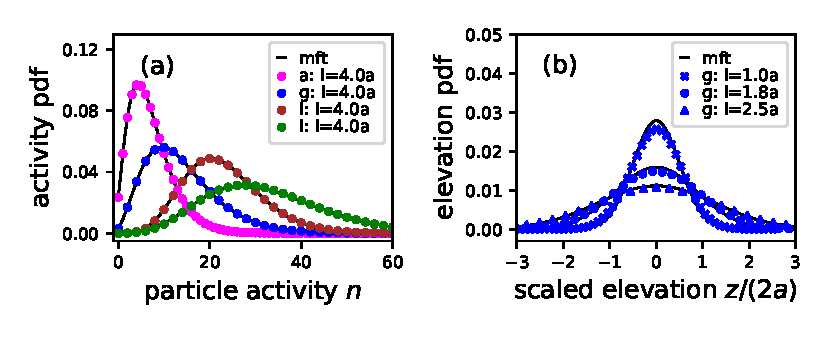
\includegraphics[width=\linewidth,keepaspectratio]{./figures/ch3/distributions.pdf}
	\caption{Panel (a) presents the probability distribution of particle activity $n$ and panel (b) presents the probability distribution of the relative number of particles $m$ for a representative subset of simulations. These distributions represent different flows from Tab. \ref{tab:anceyparams}, distinguished by color, and different values of the active layer depth $l$ (equivalently the coupling constant $\kappa$), distinguished by the marker style. The mean field theories (mft) of Eqs. \ref{eq:ancey} and \ref{eq:ou2} are displayed as solid black lines.}
	\label{fig:pdfs}
\end{figure}
The mean field equation for the particle activity $n$ (Eq.  \ref{eq:ancey}) closely represents the numerical results, and while there are small differences between numerical and analytical results for the relative number $m$ of resting particles, the numerical solutions approximately match Eq. \ref{eq:ou2}, having Gaussian profiles consistent with the assumption of a symmetric scaling between erosion and deposition rates and bed elevation changes. 


\subsection{Statistical moments of bed elevation and the particle activity}
\label{sec:elemom}

The moments of $n$ and $m$ are calculated by summing over $P(n,m)$. 
The $j$th order unconditional moment of the particle activity $n$ is defined as
\begin{equation} \langle n^j \rangle = \sum_{n}n^jP(n),\end{equation}
while the $j$th order moment of $n$ held conditional on $m$ is
\begin{equation} \langle n^j|m \rangle = \sum_{n}n^j P(n,m) .\end{equation}
The moments of $m$ show no dependence on the value of $n$. 
The mean elevation is always $\langle m \rangle = 0 $ due to the initial assumption of symmetry in the entrainment and deposition rate scaling with $m$. 


Fig. \ref{fig:var} demonstrates that the variance of bed elevations is approximately $\sigma_z^2 = z_1^2 \sigma_m^2 = \frac{1}{4\kappa}=l^2$, agreeing with the approximation in Eq. \ref{eq:ou2}; this result suggests that $l$ is a characteristic length scale of bed elevation fluctuations.
\begin{wrapfigure}{r}{0.5\textwidth}
	\centering
	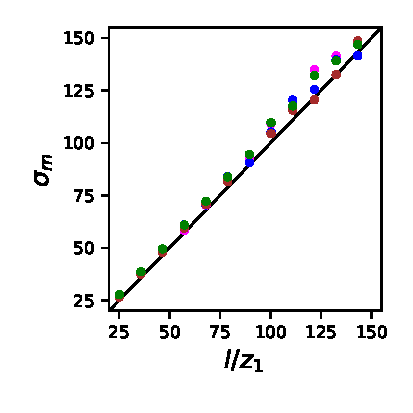
\includegraphics[width=0.5\textwidth,keepaspectratio]{./figures/ch3/variance.pdf}
	\caption{Data from all simulations demonstrating that the active layer depth $l$ characterizes bed elevation changes as described by Eq. \ref{eq:active}: $\sigma_m^2 \approx (l/z_1)^2$. }
	\label{fig:var}
\end{wrapfigure}
\indent The close correspondence between the mean field approximation and the numerical simulations in Fig. \ref{fig:pdfs} panel (a) suggests the unconditional moments of $n$ correspond closely with the \citet{Ancey2008} result. They appear identical within numerical uncertainty.

The coupling between bed elevation changes and the erosion and deposition rates develop a strong dependence of the particle activity on $m$. Fig. \ref{fig:condmoms} displays the mean shift $[\langle n |m \rangle - \langle n \rangle]/\langle n \rangle $ and the variance shift  $[\text{var}(n|m) - \text{var}(n)]/\text{var}(n)$ of the particle activity due to departures of the bed elevation from its mean position.
\begin{figure}[!htbp]
	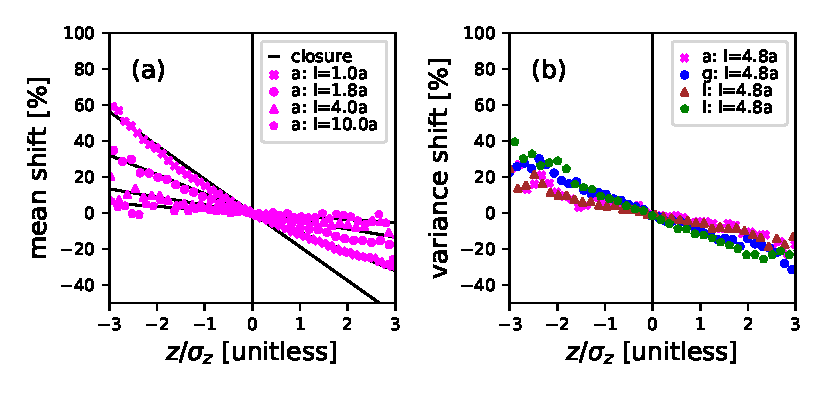
\includegraphics[width=\linewidth,keepaspectratio]{./figures/ch3/momentsuppression.pdf}
	\caption{The shifts between particle activity moments conditioned on instantaneous elevations and their over-all mean values. Panel (a) indicates the mean particle activity shift versus the bed elevation measured in units of $\sigma_z=l$. This shift displays asymmetric dependence on $m$ at the flow conditions of the \citet{Ancey2008} experiments, and departures of the bedload transport mean can be as much as 60\% when the bed is in a severely degraded state with $z\approx -3l$. The closure equation \ref{eq:closure} is plotted in panel (a). Panel (b) demonstrates a more symmetrical variance shift with some dependence on flow conditions displaying shifts of up to 20\% with bed elevations. These results indicate that bedload statistics measurements on short timescales could be severely biased by departures from the mean bed elevation.}
	\label{fig:condmoms}
\end{figure}
Figure \ref{fig:condmoms} panel (a) demonstrates that the flow conditions in Tab. \ref{tab:anceyparams} support departures of the mean particle activity by as much as 60\% from the overall mean value when the bed is in a degraded state $z\approx -3l$, and the activity can be decreased by 20\% when the bed is in an aggraded state.
The closure model (Eq. \ref{eq:closure}) used to derive the approximate bed elevation distribution (Eq. \ref{eq:ou2}) is plotted behind the conditional mean profiles in Fig. \ref{fig:condmoms} panel (a), where it appears as a crude approximation since it does not capture the asymmetry.
Nevertheless, Fig. \ref{fig:var} demonstrates the variance $1/(4\kappa)$ derived from this closure equation is representative of the numerical relationship.
For the parameters of the \citet{Ancey2008} experiments, Fig. \ref{fig:condmoms} panel (b) displays a variance shift with bed elevation changes that is less severe than the mean shift but is nevertheless appreciable, with bed elevations changing the magnitude of bedload activity fluctuations by as much as 20\%.
The summary is that bed elevation changes regulate the first and second particle activity moments, with a moment suppression effect when the bed is aggraded, and a moment enhancement effect when the bed is degraded.

\subsection{Collective entrainment and bedload activity fluctuations}
\label{sec:elecolent}
Noting that bed elevations regulate the particle activity moments, the next step is to study the influence of collective entrainment on this effect by modifying the relative proportion of the individual to collective contributions in the mean entrainment rate $E=\lambda + \sigma \langle n \rangle $.
The equilibrium condition $E=D$ implies that the fraction of entrainment due to the collective process is $f = \mu\langle n \rangle/E = \mu/\sigma$. This fraction can be used to hold $E$ constant and modify the prevalence of the collective entrainment process by setting $\lambda = E(1-f)$ and $\mu= \sigma f$. Interpolating $f$ between zero and one interpolates the particle activity component of the master equation \ref{eq:elemaster} from a purely Poissonian model to a negative binomial model, isolating the effect of collective entrainment on the particle activity statistics over a dynamic sedimentary bed.
\begin{figure}[!htbp]
	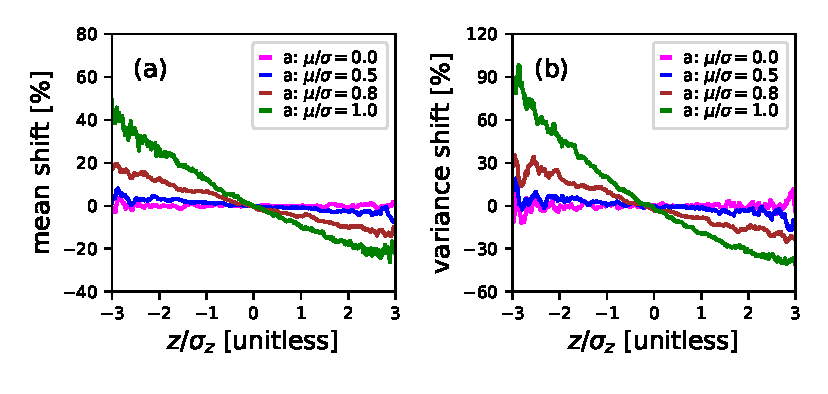
\includegraphics[width=\linewidth,keepaspectratio]{./figures/ch3/colent-suppression.pdf}
	\caption{The shift of the mean particle activity in panel (a) and its fluctuations in panel (b) with departures of the bed elevation from its mean. All simulations are at flow condition (g) from Tab. \ref{tab:anceyparams} except $\lambda$ and $\mu$ are modified to shift the fraction $f=\mu/\sigma$ of the over-all entrainment rate $E$ due to collective entrainment. Clearly, collective entrainment drives strong departures of the bedload statistics away from the mean field model (Eq. \ref{eq:ancey}) at large departures from the mean bed elevation. Panel (b) shows particle activity fluctuations suppressed by 90\% when $z\approx -3l$ and collective entrainment is the dominant process. When collective entrainment is absent, meaning $\mu/\sigma=0$, this moment regulation effect vanishes: it is a consequence of collective entrainment.}
	\label{fig:colent}
\end{figure}
Fig. \ref{fig:colent} depicts the modification of the particle activity mean and variance as the importance of collective entrainment is tuned (through $\lambda$ and $\mu$) with all other parameters fixed. When $f=0$, the bed elevation ceases to influence the particle activity mean or variance, while larger fractions increasingly enable the moment regulation effect identified in Sec. \ref{sec:elemom}.

\subsection{Resting times of sediment undergoing burial}
\label{sec:elertcdf}

\begin{figure}[!htbp]
	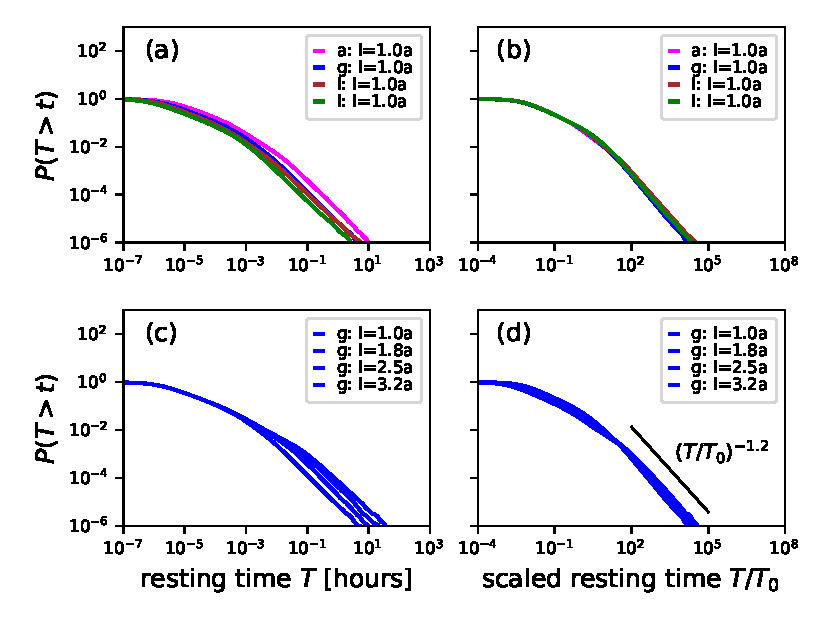
\includegraphics[width=\linewidth,keepaspectratio]{./figures/ch3/rtcdf.pdf}
	\caption{Resting time statistics scale differently with transport conditions and the bed elevation variance. Panel (a) shows differing flow conditions at a fixed $l$ value, while panel (c) shows fixed flow conditions at differing $l$. When scaled by $T_0$ (Eq. \ref{eq:time}), both types of difference collapse in the tails of the distributions, as shown in panels (b) and (d). In panels (b) and (d), the black dotted lines indicate a power law decay of the collapsed tails having parameter $\alpha\approx1.18$ .}
	\label{fig:cdfs}
\end{figure}

Resting times for sediment undergoing burial are obtained from analyzing the return times from above in the timeseries of $m$ \citep[e.g.][]{Redner2007}.
Following \citet{Voepel2013} and \citet{Martin2014}, I concentrate on a particular bed elevation $m'$, and find all time intervals separating deposition events at $m=m'$ from erosion events at $m=m'+1$.
These are the return times from above of the sedimentary bed conditional to the elevation $m'$.
Binning these conditional return times (using logarithmically-spaced bins to reduce computational load) and counting the occurrences in each bin obtains the exceedance distribution of return times $t_r$ held conditional to the elevation $m'$: $P(T>t_r|m')$.
The marginal probability distribution of bed elevations $P(m)$ displayed in Fig. \ref{fig:pdfs} panel (b) derives the unconditional exceedance distribution of resting times as a sum over all elevations \citep{Yang1971, Nakagawa1980, Voepel2013, Martin2014}: 
\begin{equation} P(T>t_r) = \sum_{m'} P(m') P(T>t_r|m') .\end{equation}
Fig. \ref{fig:cdfs} displays a representative subset of these results.
Comparing panels (a) and (c) in this figure shows two separate variations with input parameters: first, the distributions vary with the flow conditions, and second, they vary with the standard deviation of bed elevations ($l$).
However, as shown in panels (b) and u(d), a characteristic timescale $T_0$ is found to collapse away both variations.
This $T_0$ can be obtained heuristically by considering the characteristic speed of bed elevation change.
Because the mean number of grains leaving the bed per unit time is $E$ and the removal of a single grain changes the bed elevation by $z_1$ (Eq. \ref{eq:ele}), bed elevations change with a characteristic speed $v = z_1 E$.
Since the range of elevation deviations is $l$ (Fig. \ref{fig:var}), the time required for the bed to shift through this characteristic distance is $l/v$, or equivalently
\begin{equation} T_0 = \frac{l}{z_1 E}.\label{eq:time}\end{equation}
Scaling the resting time by this $T_0$ obtains the collapse shown in Fig. \ref{fig:cdfs}.
Using the log-likelihood estimation technique described by \citet{Newman2005}, the scaled resting time non-exceedance distributions are estimated to decay as a heavy tailed power law with parameter $\alpha = 1.18 \pm 0.32$ for all return times satisfying $T/T_0 > 10^3$.
These distributions are sufficiently heavy tailed to violate the central limit theorem and drive anomalous super-diffusion of bedload, a result which supports the earlier conclusions of \citet{Voepel2013} and \citet{Martin2014}.

\section{Discussion}
\label{sec:elediscussion}

\subsection{Context of the research}
Einstein developed the first stochastic models of bedload tracer diffusion \citep{Einstein1937} and the bedload flux \citep{Einstein1950}, and his ideas can be viewed as the nexus of an entire paradigm of research that extends into the present day \citep[e.g.][]{Hubbell1964, Nakagawa1976,Hassan1991,Ancey2008, Wu2019}.
These approaches aim to predict bedload transport characteristics from stochastic concepts of individual particle motions.
With some exceptions \citep{Yang1971,Nakagawa1980,Pelosi2016,Wu2019,Wu2019a}, existing descriptions are spatially one-dimensional, concentrating on the motion of grains in the downstream direction without including the vertical dimension wherein local bed elevation changes imply sediment burial \citep{Voepel2013,Martin2014} and change the mobility of surface grains \citep{Yang1971,Nakagawa1980}.

\subsection{New contributions}

This chapter has modified the birth-death approach to describe sediment transport in a control volume. This model was applied to study the interplay between bedload transport and bed elevation fluctuations and to investigate resting time distributions of sediment undergoing burial.
This model is the first description of bedload transport and bed elevations as a coupled stochastic population model based on individual grains.
Numerical solutions and analytical approximations provided negative binomial distributions of bedload activity and normal distributions of bed elevations.
Although experiments under more natural conditions with segregation processes,  migrating bedforms, or sediment supply perturbations have shown particle activity distributions with heavier tails \citep{Dhont2018,Saletti2015} and non-Gaussian bed elevations \citep{Singh2012,Aberle2006}, the results of this chapter reproduce the key features of the most controlled bed elevation \citep{Wong2007,Martin2014} and bedload transport \citep{Heyman2016,Ancey2008} experiments.

The inclusion of coupling between the bed elevation and entrainment and deposition rates revealed a novel dependence of particle activity on bed elevation changes, highlighting a new consequence of the collective entrainment process \citep{Ancey2008,Lee2018}. This coupling develops a significant variation of the particle activity moments with deviations of the bed from its mean elevation. These particle activity variations with bed elevation changes disappear in the absence of collective entrainment.

Finally, the model allowed resolution of resting times for sediment undergoing burial within the sedimentary bed. These timescales were obtained by analyzing return times from above in the bed elevation timeseries.
This analysis produces heavy-tailed power-law resting times with tail parameters sufficient to drive anomalous diffusion of bedload at long timescales.
The power-law tails were found to collapse across flow conditions using a timescale formed from the mean erosion rate and the active layer depth.

As the model in this chapter builds on earlier works describing particle activity and bed elevation changes independently, it also reduces to these works in simplified limits when the coupling between the particle activity and the local bed elevation vanishes.
With the mean field approach in Sec. \ref{sec:eleanalytical}, the \citet{Martin2014} Ornstein-Uhlenbeck model for bed elevations and the \citet{Ancey2008} birth-death model for the particle activity were derived as simplified limits of the coupled model developed in this chapter.
While the mean field description of bed elevations over-predicts the bed elevation variance by approximately a factor of two, it does capture the Gaussian shape of the bed elevation distribution, and its conclusions on the tail characteristics of resting time distributions for sediment undergoing burial are identical to the model in this chapter within the numerical uncertainty.
\citet{Martin2014} described a power-law distribution with tail parameter $\alpha \approx 1$ which falls neatly within the estimation $\alpha = 1.18 \pm 0.32$ presented here.


\subsection{Next steps for research}

The model presented in this chapter computes statistical characteristics of the bedload particle activity and bed elevation within a control volume by assuming all particles on the bed surface have similar mobility characteristics while sediment transport and bed topography are in equilibrium. In actuality, particles span a range of sizes, and spatial organization occurs both in the forces imparted to particles by the flow \citep{Shih2017,Amir2014} and in the mobility characteristics of particles on the bed surface \citep{Charru2004, Hassan2008, Nelson2014}.
Together, these factors may generate spatial correlations in particle activities that models concentrating on a single control volume will be unable to capture. 
Models chaining multiple control volumes together have shown spatial correlations in the particle activity as a result of collective entrainment \citep{Heyman2014, Ancey2015}, and similar approaches have also been applied to study correlations in turbulent flows \citep{Gardiner1983}. In light of this work, the model presented in this chapter is considered a preliminary step toward a multiple-cell model of particle activities and bed elevation changes with potential to express spatial correlations between longitudinal profile and particle activity statistics.

Like the theory developed by \citet{Martin2014}, the model Eq. \ref{eq:elemaster} produces heavy-tailed power-law resting times for sediment undergoing burial by treating bed elevation changes as an unbounded random walk with a mean reverting tendency.
This result suggests sediment burial can explain the heavy-tailed rests seen in field data \citep{Olinde2015,Bradley2017,Pretzlav2016a}. 
The resting time distributions derived in Sec. \ref{sec:elertcdf} show a divergent variance and possibly a divergent mean, since this occurs for $\alpha < 1$ \citep{Sornette2006} which is within range of the results.

Divergent mean resting time distributions present a paradox, since they imply all particles should eventually be immobile, violating the equilibrium transport assumption.
\citet{Voepel2013} demonstrated that a bounded random walk for bed elevations provides a power-law distribution that eventually transitions to a faster thin-tailed decay, allowing for power-law scaling like the result in this chapter and \citet{Martin2014} without this divergent mean paradox. 
One resolution to this issue could come from a spatially distributed model with multiple cells.
Neighboring locations might bound excessive local elevation changes through granular relaxations from gradients above the angle of repose.
In this interpretation, divergent mean power law resting time distributions may be relics of single cell models for bed elevation changes.
We should always expect a maximum depth to which the bed can degrade relative to neighboring locations; this could temper the power law tail without required the reflecting boundaries used by \citet{Voepel2013}.

Finally, this chapter presented the probability distribution functions and first and second moments of the particle activity and bed elevation, indicating novel coordination between the statistical characteristics of these quantities which deserve experimental testing.
Some relatively recent particle tracking experiments have demonstrated joint resolution of bed elevations and bedload transport \citep{Martin2014,Heyman2016}.
A suitably designed experiment using this methodology could test the prediction that bed elevations regulate particle activity statistics, as essentially represented in Figs. \ref{fig:condmoms} and \ref{fig:colent}. 

Many other statistical characteristics of bedload transport have been left for future studies. 
For example, the dependence of bedload transport \citep{Saletti2015,Singh2009} and bed elevation statistics \citep{Aberle2006, Singh2009,Singh2012} on the spatial and temporal scales over which they are observed is an emerging research topic which was previously referenced in Sec. \ref{sec:renewal}.
Whether bed elevation distributions are also scale-dependent like the sediment flux distribution of Ch. \ref{ch:flux} is an interesting question for future research.

\section{Summary}
\label{sec:eleconclusion}

This chapter presented a stochastic model for particle activity and local bed elevations including feedbacks between elevation changes and sediment transport.
This model includes collective entrainment, whereby moving particles tend to destabilize stationary ones.
The model was analyzed using a mixture of numerical and analytical methods, and two key results were presented:
\begin{enumerate}
	\item Resting times for sediment undergoing burial lie on a heavy-tailed power law distributions with tail parameter $\alpha \approx 1.2$;
	\item Collective entrainment generates a statistical regulation effect, whereby bed elevation changes modify the mean and variance of the particle activity by as much as 90\%: this effect vanishes when collective entrainment is absent.
\end{enumerate}
These results imply measurements of bedload transport statistics could be biased at observation timescales smaller than adjustments of the bed elevation timeseries when collective entrainment occurs.
The next step is to generalize the model in this chapter to a multi-cell framework to study channel morphodynamics in a stochastic framework.

%%!TEX root = diss.tex

\chapter{Burial-induced three-range diffusion in sediment transport}
\label{ch:downDiff}

Many environmental problems including channel morphology \citep{Hassan2017}, contaminant transport \citep{Macklin2006}, and aquatic habitat restoration \citep{Gaeuman2017} rely on our ability to predict the diffusion characteristics of coarse sediment tracers in river channels.
Diffusion is quantified by the time dependence of the positional variance $\sigma_x^2$ of a group of tracers.
With the scaling $\sigma_x^2 \propto t$, the diffusion is said to be normal, since this is found in the classic problems \citep{Einstein1905}.
However, with the scaling $\sigma_x^2 \propto t^\gamma$ with $\gamma \neq 1$, the diffusion is said to be anomalous \citep{Sokolov2012}, with $\gamma>1$ defining super-diffusion and $\gamma<1$ defining sub-diffusion \citep{Metzler2000}.
\citet{Einstein1937} developed one of the earliest models of bedload diffusion to describe a series of flume experiments \citep{Ettema2004}.
Interpreting individual bedload trajectories as a sequence of random steps and rests, Einstein originally concluded that a group of bedload tracers undergoes normal diffusion.

More recently, Nikora et al. realized coarse sediment tracers can show either normal or anomalous diffusion depending on the length of time they have been tracked \citep{Nikora2001a,Nikora2002}.
From numerical simulations and experimental data, Nikora et al. discerned ``at least three'' scaling ranges $\sigma_x^2 \propto t^\gamma$ as the observation time increased.
They associated the first range with ``local'' timescales less than the interval between subsequent collisions of moving grains with the bed, the second with ``intermediate'' timescales less than the interval between successive resting periods of grains, and the third with ``global'' timescales composed of many intermediate timescales.
Nikora et al. proposed super-diffusion in the local range, anomalous or normal diffusion in the intermediate range, and sub-diffusion in the global range.
They attributed these ranges to ``differences in the physical processes which govern the local, intermediate, and global trajectories'' of grains \citep{Nikora2001a}, and they called for a physically based model to explain the diffusion characteristics \citep{Nikora2002}.

Experiments support the Nikora et al. conclusion of multiple scaling ranges \citep{Martin2012,Fathel2016}, but they do not provide consensus on the expected number of ranges or their scaling properties.
This lack of consensus probably stems from resolution issues.
For example, experiments have tracked only moving grains, resolving the local range \citep{Furbish2012,Furbish2017,Fathel2016}; grains resting on the bed surface between movements, resolving the intermediate range \citep{Einstein1937,Yano1969,Nakagawa1976}; grains either moving or resting on the bed surface, likely resolving local and intermediate ranges \citep{Martin2012}; or grains resting on the surface after floods, likely resolving the global range \citep{Phillips2013,Bradley2017}. 
At long timescales, a significant fraction of tracers become buried under the bed surface \citep{Hassan1991,Hassan2013,Ferguson2002a,Haschenburger2013,Papangelakis2016}, meaning burial dominates long term diffusion characteristics \citep{Bradley2017,Martin2014,Voepel2013}, possibly at global or even longer ``geomorphic'' timescales \citep{Hassan2017} than Nikora et al. originally considered.
As a result, three diffusion ranges can be identified by patching together multiple data-sets \citep{Zhang2012,Nikora2002}, but they are not resolved by any one data-set.

Newtonian bedload trajectory models also show multiple diffusion ranges, although they also do not provide consensus on the expected number of ranges or their scaling properties. 
The majority of these models predict two ranges of diffusion (local and intermediate) without predicting a global range.
Among these, \citet{Nikora2001a} used synthetic turbulence \citep{Kraichnan1970} with a discrete element method for the granular phase \citep{Cundall1979}; \citet{Bialik2012} used synthetic turbulence with a random collision model \citep{Sekine1992}; and \citet{Fan2016} used a Langevin equation with probabilistic rests.
To my knowledge, only \citet{Bialik2015} have claimed to capture all three ranges from a Newtonian approach.
They incorporated a second resting mechanism into their earlier model \citep{Bialik2012}, implicitly suggesting that three diffusion ranges could result from two distinct timescales of sediment rest.
However, Newtonian approaches have not evaluated the effect of sediment burial on tracer diffusion, probably due to the long simulation timescales required. 

Random walk bedload diffusion models constructed in the spirit of \citet{Einstein1937} provide an alternative to the Newtonian approach and can include a second timescale of rest by incorporating sediment burial.
Einstein originally modeled bedload trajectories as instantaneous steps interrupted by durations of rest lying on statistical distributions \citep{Hassan1991}, but this generates only one range of normal diffusion \citep{Einstein1937,Hubbell1964,Nakagawa1976}.
Recently, researchers have generalized Einstein's model in a few different ways to describe multiple diffusion ranges.
\citet{Lisle1998} and \citet{Lajeunesse2017} promoted Einstein's instantaneous steps to motion intervals with random durations and a constant velocity, providing two diffusion ranges -- local and intermediate.
\citet{Wu2019} retained Einstein's instantaneous steps but included the possibility that grains can become permanently buried as they rest on the bed, also providing two diffusion ranges -- intermediate and global. 
These earlier works suggest the minimal required components to model three bedload diffusion ranges: (1) exchange between motion and rest intervals and (2) the sediment burial process.

In this study, I incorporate these two components into Einstein's original approach to describe three diffusion ranges with a physically based model, as called for by \citet{Nikora2002}.
Einstein was a giant in river geophysics and fostered an entire paradigm of research leveraging and generalizing his stochastic methods \citep{Hubbell1964, Yano1969, Yang1971, Gordon1972, Nakagawa1976,Paintal1971}.
Einstein's model can be viewed as a pioneering application of the continuous time random walk (CTRW) developed by \citet{Montroll1965} in condensed matter physics to describe the diffusion of charge carriers in solids.
To incorporate motion intervals and sediment burial, I utilize the multi-state CTRW formalism developed by \citet{Weiss1976, Weiss1994} that extends the CTRW of \citet{Montroll1965}.
Below, I develop and solve the model in Sec. \ref{sec:model}. Then, I discuss the predictions of this model, present its implications for local, intermediate, and global ranges of bedload diffusion, and suggest next steps for bedload diffusion research in Secs. \ref{sec:discussion} and \ref{sec:conclusion}.

\section{Bedload trajectories as a multi-state random walk}
\label{sec:model}
\subsection{Assumptions of the burial model}
\label{sec:assumptions}
Particle trajectories are formulated as a three-state random walk where the states are motion, surface rest, and burial. These states are labeled as $i=2$ (motion), $i=1$ (rest), and $i=0$ (burial).
The target is the probability distribution $p(x,t)$ to find a grain at position $x$ and time $t$ if it is known to have started with the initial distribution $p(x,0)=\delta(x)$.
Times spent moving or resting on the surface are characterized by exponential distributions $\psi_M(t)=k_2e^{-k_2 t}$ and $\psi_1(t) = k_1e^{-k_1t}$, since numerous experiments show thin-tailed distributions for these quantities \citep{Fathel2015,Roseberry2012,Einstein1937,Ancey2006,Martin2012}. The end results will not be contingent on the specific distributions chosen, since all thin-tailed distributions provide similar diffusion characteristics in random walks \citep{Weiss1994,Weeks1998}.
Grains in motion are considered to have a characteristic velocity $v$ \citep{Lisle1998,Lajeunesse2017}, and burial is modeled as long lasting enough to be effectively permanent \citep{Wu2019}, with grains resting on the surface having a probability per unit time $\kappa$ to become buried.
This means $\Phi(t) = e^{-\kappa t}$ represents the probability that a grain is not buried after resting for a time $t$, while $1-\Phi(t)$ represents the probability that it is buried.
The initial conditions are specified with probabilities $\theta_1$ and $\theta_2$ to be in rest or motion at $t=0$. Normalization requires $\theta_1+\theta_2=1$.

\subsection{Governing equations}
With these assumptions, the governing equations for the set of probabilities $\om_{ij}(x,t)$ that a transition occurs from state $i$ to state $j$ at position $x$ and time $t$ can be derived using the statistical physics approach to multi-state random walks \citep{Weiss1994,Schmidt2007,Weeks1998}.
Denoting by $g_{ij}(x,t)$ the probability for a particle to move a distance $x$ in a time $t$ within the state $i$ before it transitions to the state $j$, the transition probabilities $\om_{ij}(x,t)$ sum over all possible paths to the state $i$ from previous locations and times:
\be \om_{ij}(x,t) = \theta_i g_{ij}(x,t) + \sum_{k=0}^2 \int_0^x dx' \int_0^t dt' \om_{ki}(x',t')g_{ij}(x-x',t-t').\label{eq:g1}\ee
Defining another set of probabilities $G_i(x,t)$ that a particle moves by a distance $x$ in a time $t$ within the state $i$ and possibly remains within the state, a similar sums over paths for the probabilities to be in the state $i$ at $x$, $t$ produces: 
\be p_i(x,t) = \theta_i G_i(x,t) + \sum_{k=0}^2 \int_0^x dx' \int_0^t dt' \om_{ki}(x',t')G_i(x-x',t-t').\label{eq:g2}\ee
Finally, the overall probability to be at position $x$ at time $t$ is
\be p(x,t) = \sum_{k=0}^2 p_k(x,t). \ee
This joint density is completely determined from the solutions of Eqs. \ref{eq:g1} and \ref{eq:g2} given specification of the distributions $g_{ij}$ and $G_i$.


\subsection{Joint probability distribution of particle position with burial}
\label{sec:solution}

These distributions can be constructed from the assumptions described in Sec. \ref{sec:assumptions}.
Since particles resting on the bed surface become buried in a time $t$ with probability $\Phi(t)$, and resting times are distributed as $\psi_1(t)$, these assumptions obtain $g_{12}(x,t) = \delta(x)k_1e^{-k_1t}e^{-\kappa t}$ and $g_{10}(x,t) = \delta(x) k_1 e^{-k_1 t}(1-e^{-\kappa t})$. Since motions have velocity $v$ for times distributed as $\psi_2(t)$, the assumptions provide $g_{21}(x,t) = \delta(x-vt)k_2e^{-k_2 t}$.
Since burial is quasi-permanent, all other $g_{ij} = 0$.
The $G_i$ are constructed in the same way except using the cumulative probabilities $\int_t^\infty dt'\psi_i(t) = e^{-k_i t}$, since these characterize motions and rests that are ongoing \citep{Weiss1994}.
Using the cumulative probabilities provides $G_1(x,t) = \delta(x)e^{-k_1t}$ and $G_2(x,t) = \delta(x-vt)e^{-k_2 t}$.

Eqs. \ref{eq:g1} and \ref{eq:g2} with these $g_{ij}$ and $G_i$ are solved using Laplace transforms in space and time $(x,t \rightarrow 
\eta,s).$ This method, similar to \citet{Weeks1998}, unravels the convolution structure of these equations, eventually producing
\be \tilde{p}(\eta,s) = \frac{1}{s}\frac{(s+\kappa + k')s  + \theta_1(s+\kappa )\eta v+ \kappa k_2}{(s+\kappa+k_1)\eta v+(s+\kappa+k')s + \kappa k_2}, \label{eq:diffnicedist}\ee
where $k' = k_1 + k_2$. As explained in appendix Sec. \ref{sec:appendixA}, inverting this result using known Laplace transforms \citep{Prudnikov1992a,Arfken1985} obtains
\begin{align}
	\begin{split}
		p(x,t) = \theta_1&\Big[1-\frac{k_1}{\kappa+k_1}\Big(1-e^{-(\kappa+k_1)t}\Big)\Big]\delta(x) \\ &+ \frac{1}{v}e^{-\Omega \tau - \xi}\Big(\theta_1\Big[k_1\mathcal{I}_0\big(2\sqrt{\xi\tau}\big) + k_2\sqrt{\frac{\tau}{\xi}}\mathcal{I}_1\big(2\sqrt{\xi\tau}\big)\Big] \\ 
		&+ \theta_2\Big[k_1\delta(\tau) + k_2 \mathcal{I}_0\big(2\sqrt{\xi\tau}\big)+k_1 \sqrt{\frac{\xi}{\tau}}\mathcal{I}_1\big(2\sqrt{\xi\tau}\big)\Big]\Big) \\
		&+ \frac{1}{v}\frac{\kappa k_2}{\kappa + k_1}e^{-\kappa \xi/(\kappa + k_1)}\Big[(\theta_1/\Omega)\mathcal{Q}_2(\xi/\Omega,\Omega\tau) + \theta_2 \mathcal{Q}_1(\xi/\Omega,\Omega\tau)\Big]
		\label{eq:pdf}
	\end{split}
\end{align}
for the joint distribution that a tracer is found at position $x$ at time $t$.
This result generalizes the earlier results of \citet{Lisle1998} and \citet{Einstein1937} to include sediment burial.
This equation uses the shorthand notations $\xi = k_2 x/v$, $\tau = k_1(t-x/v)$, and $\Omega = (\kappa+k_1)/k_1$ \citep[cf.][]{Lisle1998}. The $\mathcal{I}_\nu$ are modified Bessel functions of the first kind and the $\mathcal{Q}_\mu$ are generalized Marcum Q-functions defined by $\mathcal{Q}_\mu(x,y) = \int_0^y e^{-z-x}(z/x)^{(\mu-1)/2}\mathcal{I}_{\mu-1}(2\sqrt{xz})dz $ and originally devised for radar detection theory \citep{Marcum1960,Temme1996}. 
The Marcum Q-functions derive from the burial process.
Because resting grains can become buried with an exponential probability, while the probability that particles rest follows a modified Bessel distribution \citep{Einstein1937,Lisle1998}, evaluating the probability that particles rest and become buried generates the Q-function convolution structure. 

\begin{figure}[!htbp]
	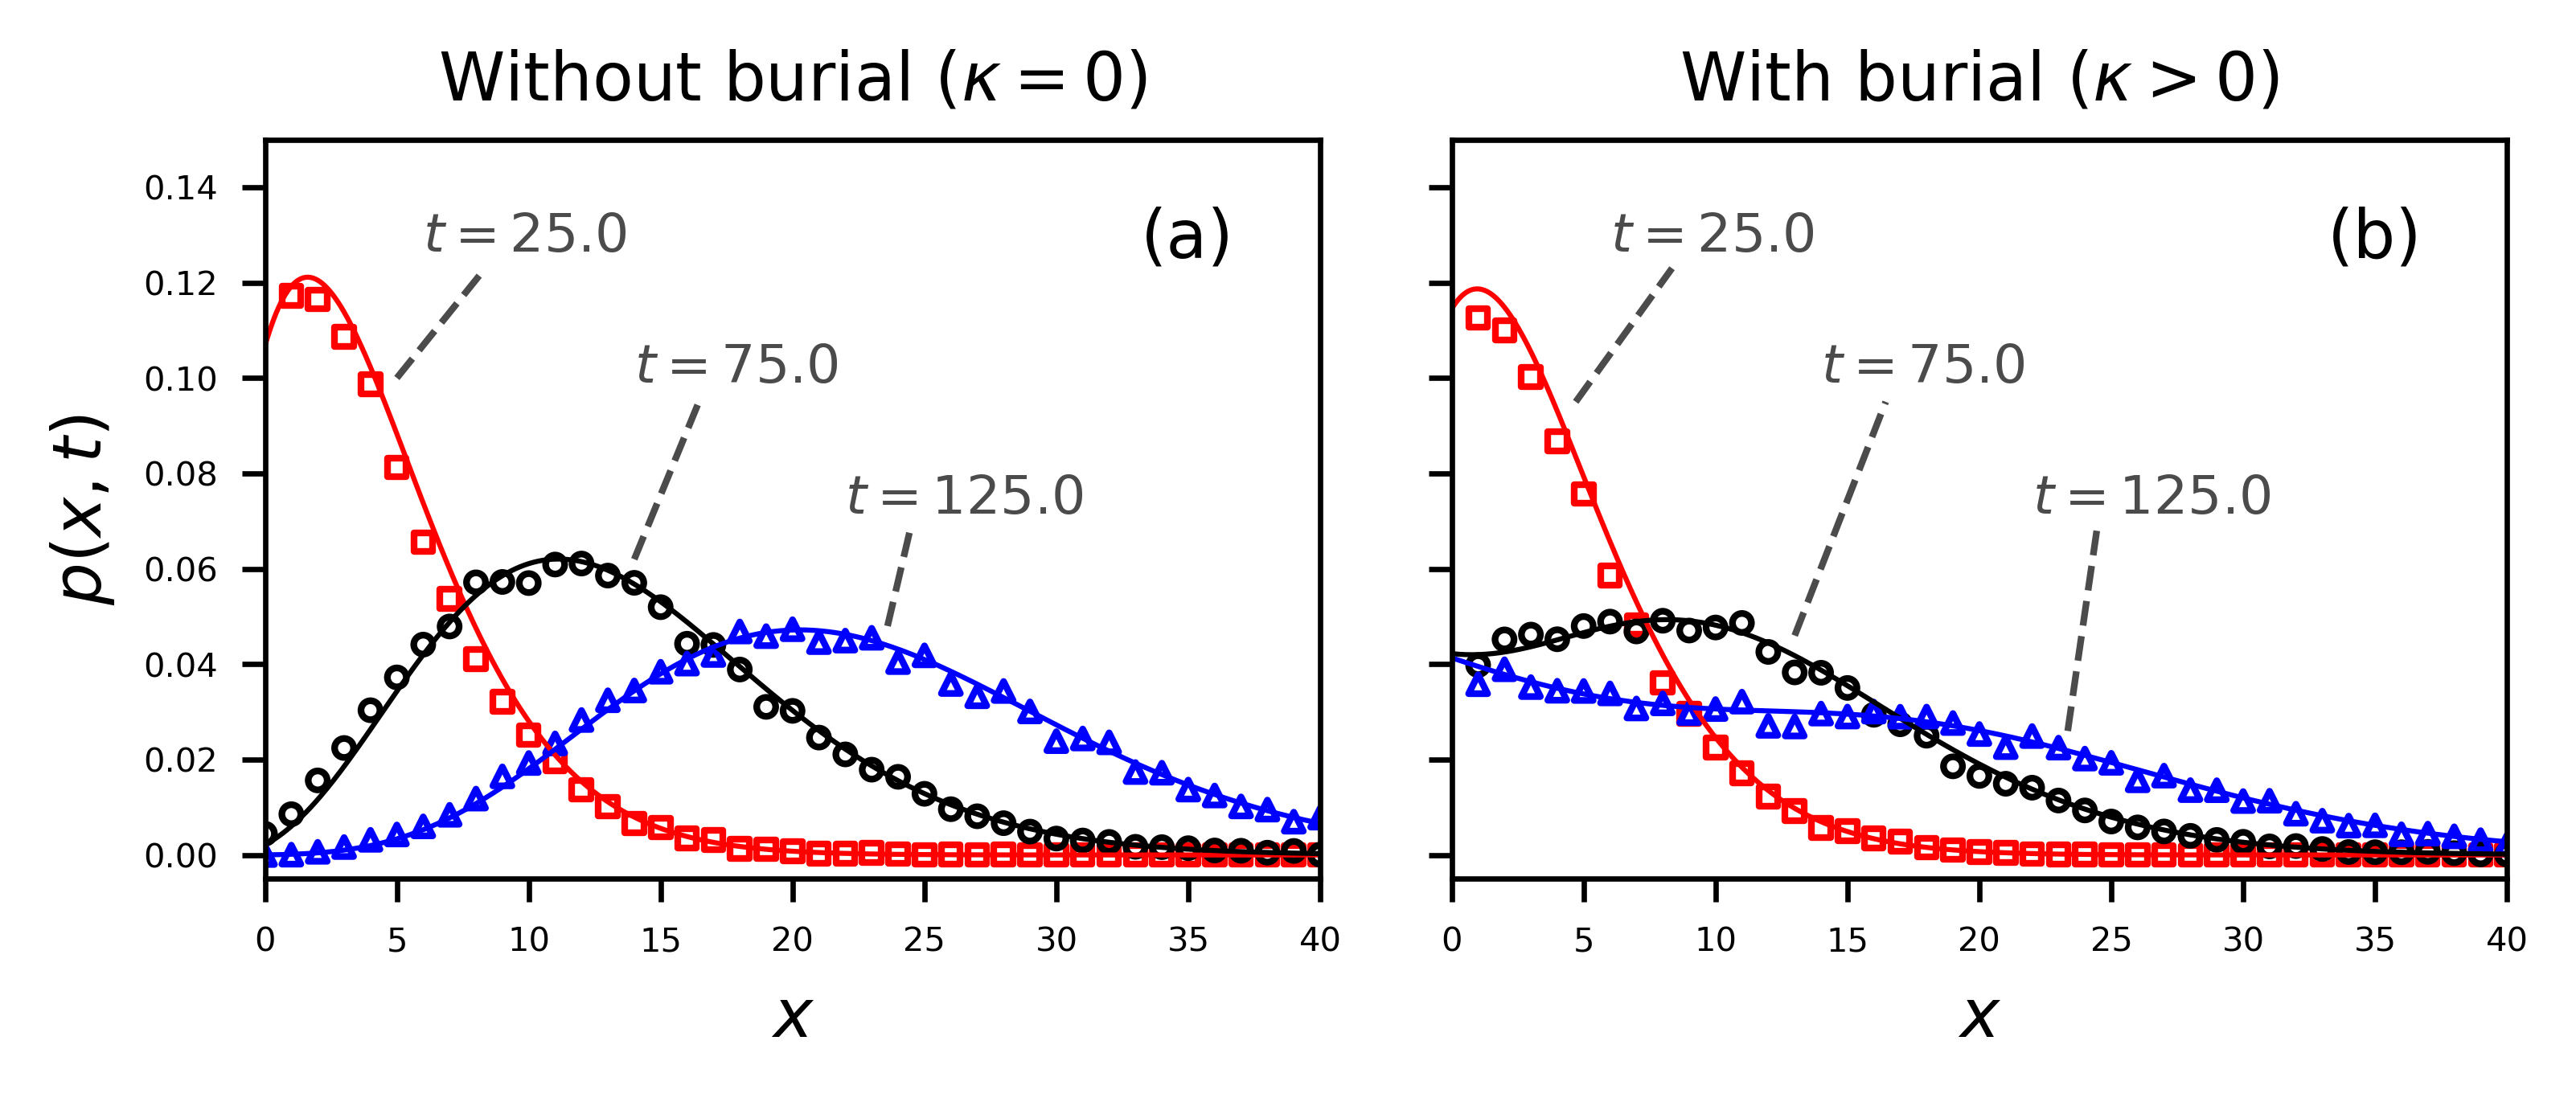
\includegraphics[width=\linewidth,keepaspectratio]{./figures/ch4/pdf-plot.png}
	\caption{Joint distributions for a grain to be at position $x$ at time $t$ are displayed for the choice $k_1=0.1$, $k_2=1.0$, $v=2.0$. Grains are considered initially at rest ($\theta_1=1$, $\theta_2=0$). The solid lines are the analytical distribution in Eq. \ref{eq:pdf}), while the points are numerically simulated, showing the correctness of the derivations. Colors pertain to different times. Units are unspecified, since the aim is to demonstrate the general characteristics of $p(x,t)$. Panel (a) shows the case $\kappa=0$ -- no burial. In this case, the joint distribution tends toward Gaussian at large times \citep{Einstein1937,Lisle1998}. Panel (b) shows the case when grains have rate $\kappa = 0.01$ to become buried while resting. Because of burial, the joint distribution tends toward a more uniform distribution than Gaussian.
		\label{fig:diffpdfs}}
\end{figure}

Fig. \ref{fig:diffpdfs} depicts the distribution Eq. \ref{eq:pdf} alongside simulations generated by a direct method based on evaluating the cumulative transition probabilities between states on a small time-step \citep{Barik2006}.
When grains do not become buried, as in panel (a) of Fig. \ref{fig:diffpdfs}, the distribution becomes Gaussian-like at relatively large observation times, exemplifying normal diffusion and satisfying the central limit theorem.
When grains become buried, as in panel (b) of Fig. \ref{fig:diffpdfs},  the Q-function terms prevent the distribution from approaching a Gaussian at large timescales, exemplifying anomalous diffusion \citep{Weeks1998} and violating the central limit theorem \citep{Metzler2000,Schumer2009}.


\subsection{Downstream diffusion}

To obtain an analytical formula for tracers diffusing downstream while they gradually become buried, the first two moments of position are derived by taking derivatives with respect to $\eta$ of the Laplace space distribution (Eq. \ref{eq:diffnicedist}) using an approach similar to \citet{Shlesinger1974} and \citet{Weeks1998}. These moments produce the positional variance $\sigma_x^2 = \bra x^2\ket - \bra x \ket^2$. 
The first two moments are
\begin{align}
	\bra x(t) \ket &= A_1 e^{(b-a)t}+B_1e^{-(a+b)t}+C_1, \label{eq:mean}\\
	\bra x^2(t) \ket &= A_2(t)e^{(b-a)t}+B_2(t)e^{-(a+b)t}+C_2, \label{eq:second}
\end{align}
so the variance is 
\be \sigma_x^2(t) = A(t)e^{(b-a)t} + B(t)e^{-(a+b)t} + C(t). \label{eq:var}\ee
In these equations, $a = (\kappa + k_1+k_2)/2$ and $b = \sqrt{a^2-\kappa k_2}$ are effective rates having dimensions of inverse time, while the $A$, $B$, and $C$ factors are provided in Tab. \ref{table:params}.

%\\
%		&\hspace{1cm}
\begin{table}[!h]
	\centering
	%\begin{wraptable}{r}{width=5.5cm}
	\caption{Abbreviations used in the expressions of the mean (Eq. \ref{eq:mean}), second moment (Eq. \ref{eq:second}) and variance (Eq. \ref{eq:var}) of bedload tracers.}
	\label{table:params}
	\small
	\begin{tabular}{c}
		\toprule
		$\begin{aligned}[t]
			&A_1 = \frac{v}{2b}\big[\theta_2+\frac{k_1+\theta_2\kappa}{b-a}\big] \\
			&B_1 = -\frac{v}{2b}\big[\theta_2-\frac{k_1+\theta_2 \kappa}{a+b}\big] \\
			&C_1 =  -\frac{v}{2b}\big[\frac{k_1+\theta_2 \kappa}{b-a}+\frac{k_1+\theta_2 \kappa}{a+b}\big]\\
			&A_2(t) = \frac{v^2}{2b^3}\Big[(bt-1)[k_1+\theta_2(2\kappa + k_1 + b-a)]+\theta_2b 
			+ \frac{(\kappa+k_1)(\theta_2\kappa+k_1)}{(b-a)^2}[(bt-1)(b-a)-b]\Big]\\
			&B_2(t) = \frac{v^2}{2b^3}\Big[(bt+1)[k_1 + \theta_2(2\kappa+k_1-a-b)]+\theta_2b
			-\frac{(\kappa+k_1)(\theta_2\kappa+k_1)}{(a+b)^2}[(bt+1)(a+b)+b]\Big]\\
			&C_2 = \frac{v^2}{2b^3}(\kappa+k_1)(\theta_2 \kappa + k_1)\Big[\frac{2b-a}{(b-a)^2}+\frac{a+2b}{(a+b)^2}\Big]\\
			&A(t) = A_2(t)-2A_1C_1 - A_1^2\exp[(b-a)t]\\
			&B(t) = B_2(t)-2B_1C_1 - B_1^2\exp[-(a+b)t]\\
			&C(t) = C_2-C_1^2-2A_1B_1\exp[-2at]\\			
		\end{aligned}$\\
		\bottomrule
	\end{tabular}
	%\end{wraptable}
	\vspace{-0.5cm}
\end{table}
The positional variance Eq. \ref{eq:var} is plotted in Fig. \ref{fig:diffvar} for conditions $\theta_1=1$ and $k_2\gg k_1 \gg \kappa$.
The notation ``$\gg$'' is interpreted in this context to mean ``of at least an order of magnitude greater''.
These conditions are most relevant to tracers in gravel-bed rivers, since they represent that grains are initially at rest \citep{Hassan1991,Wu2019}, motions are typically much shorter than rests \citep{Einstein1937,Hubbell1964}, and burial requires a much longer time than typical rests  \citep{Ferguson2002,Hassan1994,Haschenburger2013}.
Figure \ref{fig:diffvar} demonstrates that under these conditions the variance (Eq. \ref{eq:var}) shows three diffusion ranges with approximate power law scaling ($\sigma_x^2 \propto t^\gamma$) that are identified as the local, intermediate, and global ranges proposed by Nikora et al., followed by a fourth range of no diffusion ($\sigma_x^2 = \text{const}$) stemming from the burial of all tracers. 
Following \citet{Hassan2017} I suggest to call the fourth range "geomorphic", since any further transport in this range can occur only if scour re-exposes buried grains to the flow \citep{Nakagawa1980,Voepel2013,Martin2014,Wu2019a}.

\begin{figure}[!htbp]	
	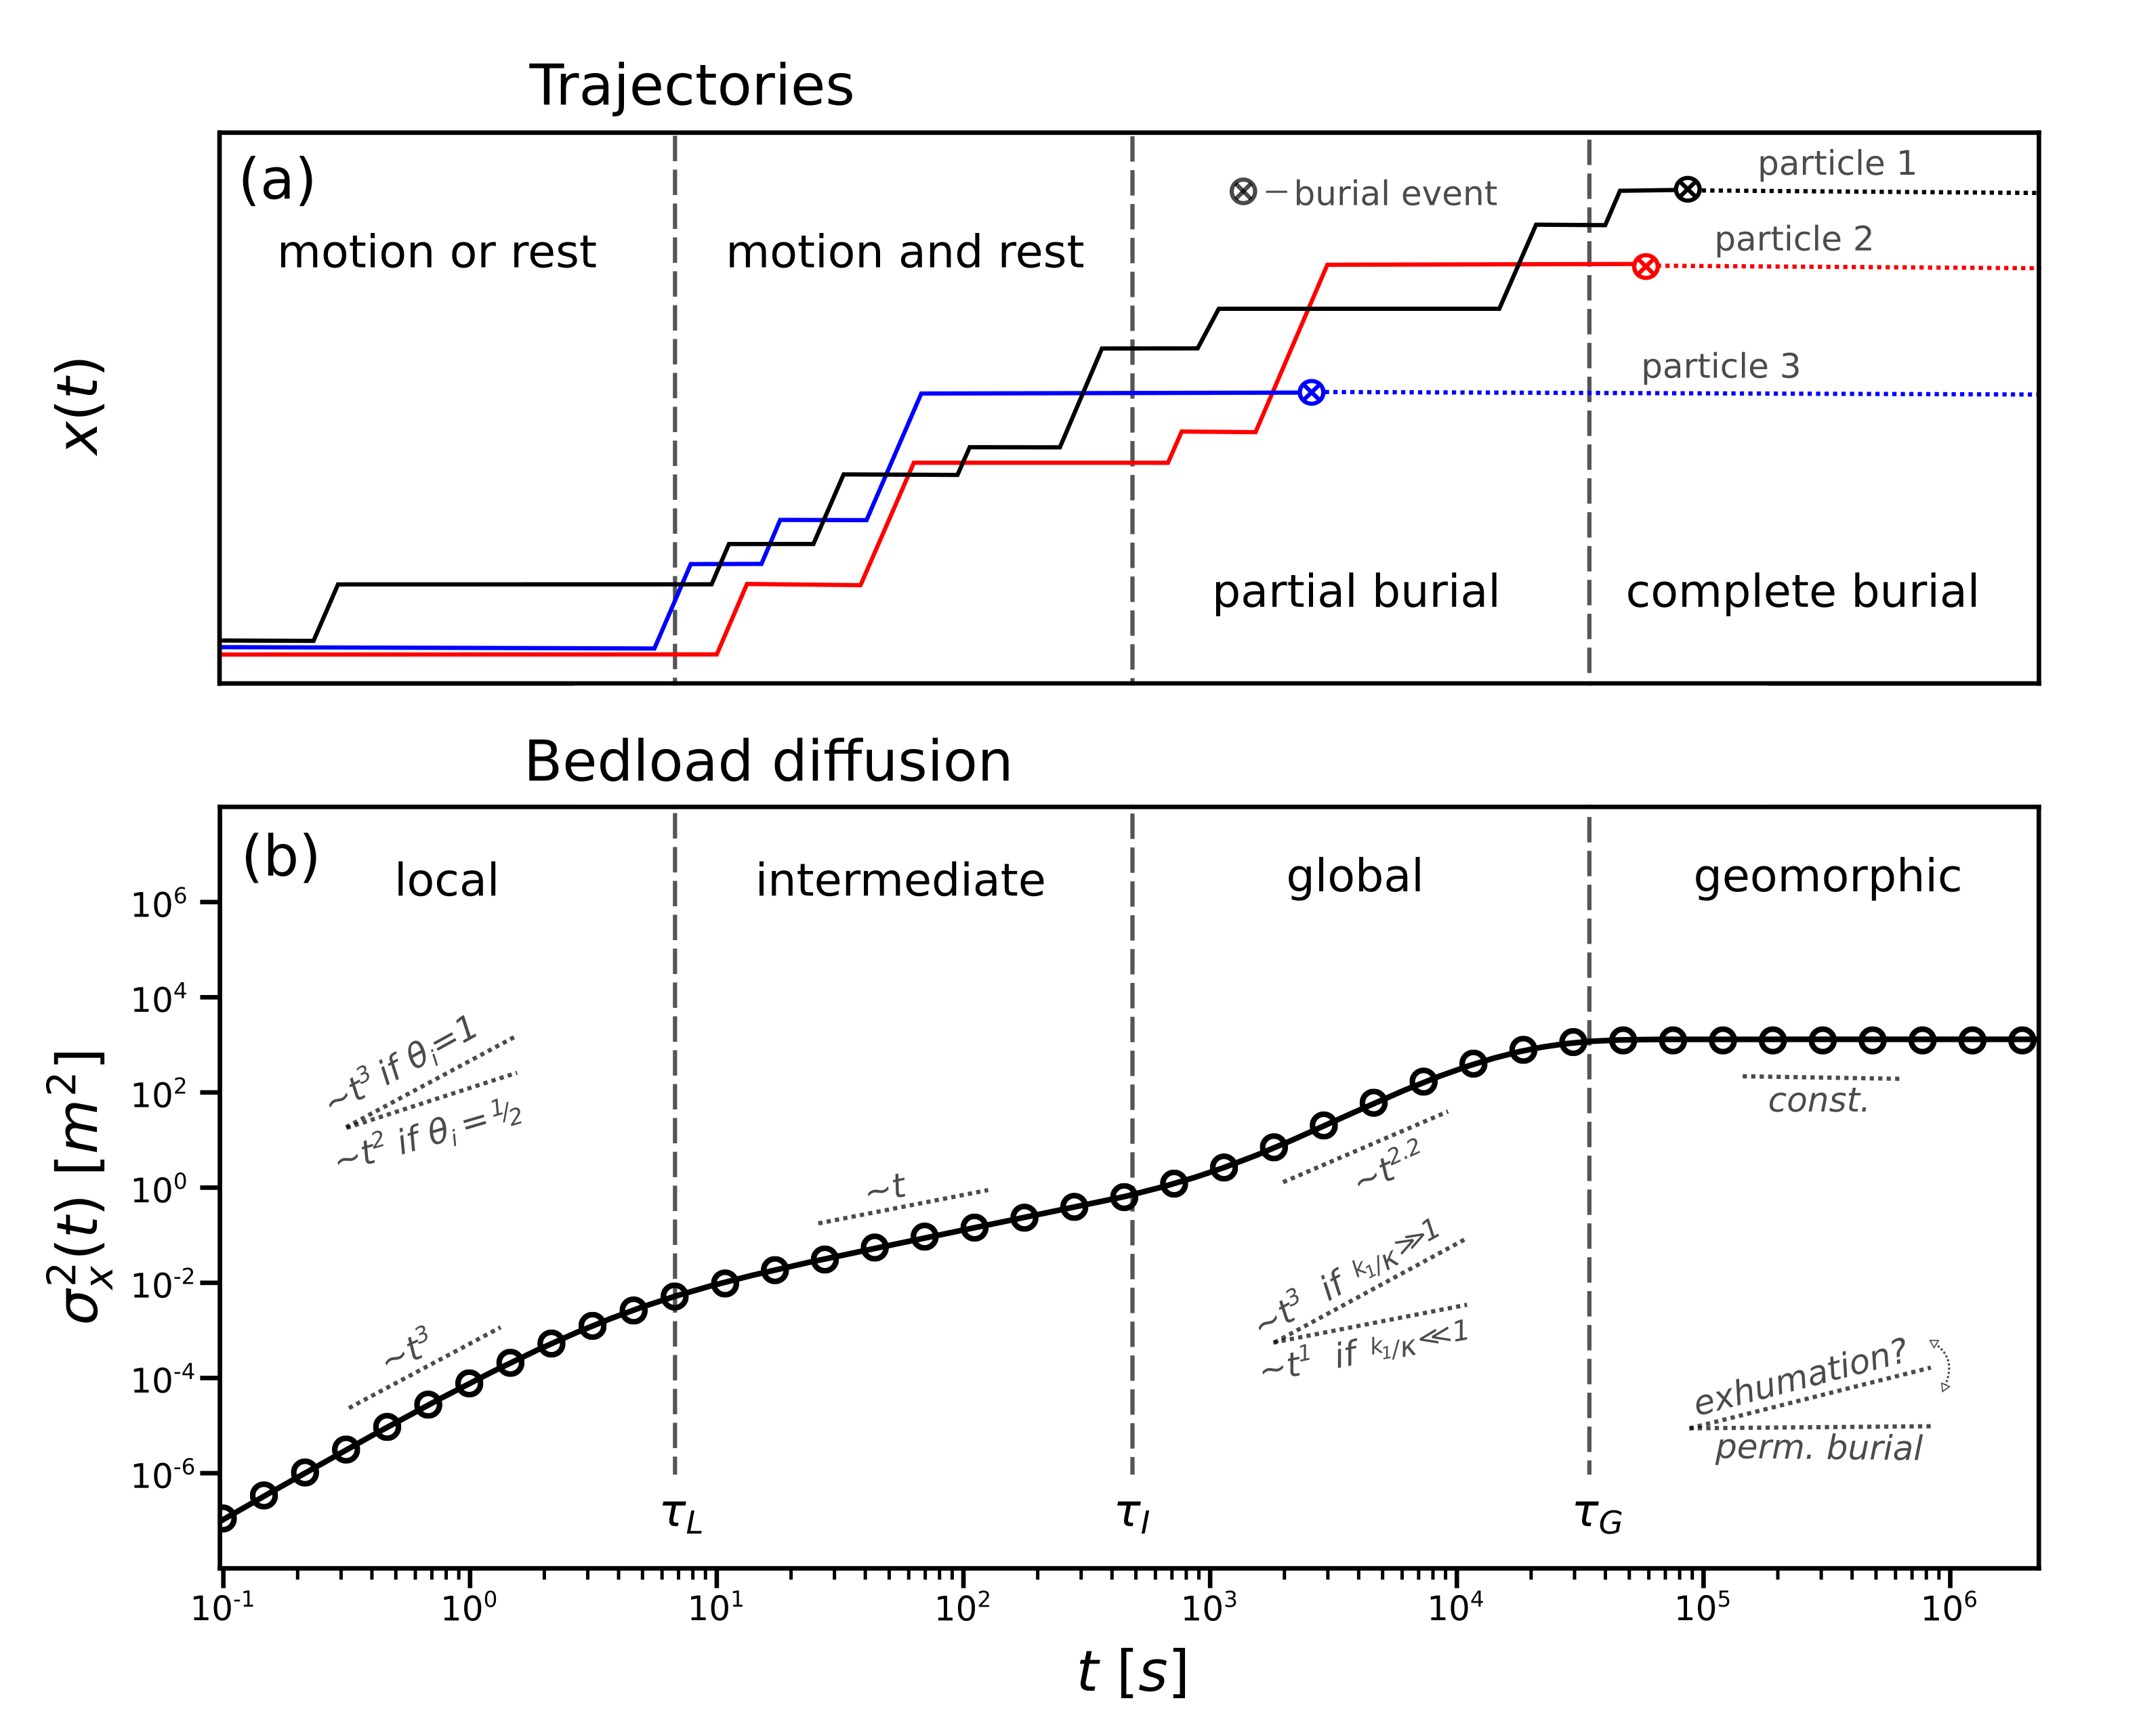
\includegraphics[width=\linewidth,keepaspectratio]{./figures/ch4/diffusion.png}
	\caption{Panel (a) sketches conceptual trajectories of grains, while panel (b) depicts Eq. \ref{eq:var} with mean motion time $1.5$ s, rest time $30.0$ s, and velocity $0.1$ m/s. The burial timescale is $7200$ s (two hours), and grains start from rest ($\theta_1=1$). The solid line is Eq. \ref{eq:var} and points are numerically simulated. Panel (b) demonstrates four distinct scaling ranges of $\sigma_x^2$: local, intermediate, global, and geomorphic. The first three are diffusive. Crossover times $\tau_L$, $\tau_I$, and $\tau_G$ divide the ranges. Slope keys demonstrate the scaling $\sigma_x^2 \propto t^\gamma$ in each range. Panel (a) demonstrates that different mixtures of motion, rest, and burial states generate the ranges. At local timescales, grains usually either rest or move; at intermediate timescales, they transition between rest and motion; at global timescales, they transition between rest, motion, and burial; and at geomorphic timescales, all grains become buried.
	}
	\label{fig:diffvar}
\end{figure}

\subsection{Diffusion exponents and three-range scaling}
\label{sec:amidonenow}

Two limiting cases of Eq. \ref{eq:var} provide the scaling exponents $\gamma$ of the diffusion $\sigma_x^2 \propto t^\gamma$ in each range. Limit (1) represents times so short that a negligible amount of sediment burial has occurred, $t\ll 1/\kappa$, while limit (2) represents times so long motion intervals appear as instantaneous steps of mean length $l=v/k_2$, $1/k_2 \rightarrow 0$ while $v/k_2 = \text{constant}$.
Limit (1) provides local exponent $2 \leq \gamma \leq 3$ depending on the initial conditions $\theta_i$, and intermediate exponent $\gamma=1$.
If grains start in motion or rest exclusively, meaning one $\theta_i = 0$, the local exponent is $\gamma=3$, while if grains start in a mixture of motion and rest states, meaning neither $\theta_i$ is zero, the local exponent is $\gamma=2$.
Limit (2) provides global exponent $1 \leq \gamma \leq 3$ depending on the relative importance of $\kappa$ and $k_1$.
The extreme $k_1/\kappa \ll 1$ produces $\gamma=1$ in the global range, while the opposite extreme $k_1/\kappa \rightarrow \infty$ produces $\gamma=3$.
To summarize, when $k_2\gg k_1 \gg \kappa$ so all three diffusion ranges exist, Eq. \ref{eq:var} implies:
\begin{enumerate}
	\item local range super-diffusion with $2<\gamma<3$ depending on whether grains start from purely motion or rest ($\gamma=3$) or from a mixture of both states ($\gamma=2$),
	\item intermediate range normal diffusion $\gamma=1$ independent of model parameters, and
	\item global range super-diffusion $1<\gamma<3$ depending on whether burial happens relatively slowly ($\gamma \rightarrow 1$) or quickly ($\gamma \rightarrow 3$) compared to surface resting times.
\end{enumerate}
Finally, the burial of all tracers generates a geomorphic range of no diffusion.

\section{Discussion}
\label{sec:discussion}

\subsection{Local and intermediate ranges with comparison to earlier work}

This chapter has extended \citet{Einstein1937} by including motion, rest, and burial processes in a multi-state random walk \citep{Weiss1994,Weeks1998} to demonstrate that a group of bedload tracers moving downstream while gradually becoming buried will generate a super-diffusive local range \citep{Martin2012,Fathel2016,Witz2018}, a normal-diffusive intermediate range \citep{Nakagawa1976,Yano1969}, and a super-diffusive global range \citep{Bradley2017, Bradley2010} before the diffusion eventually terminates in a geomorphic range \citep{Hassan2017}.
\citet{Nikora2002} highlighted the need for such a physical description, although they suggested to use a two-state random walk between motion and rest states with heavy-tailed resting times, and they did not discuss sediment burial.
However, other works have demonstrated that a two-state walk with heavy-tailed rests provides two diffusion ranges -- not three \citep{Weeks1996,Fan2016}, and although heavy-tailed resting times have been documented for surface particles \citep{Liu2019,Fraccarollo2019}, they are more often associated with buried particles \citep{Martin2012,Martin2014,Voepel2013,Olinde2015,Pelosi2016, Pierce2020a}, while surface particles retain light-tailed resting times \citep{Einstein1937,Yano1969,Ancey2006,Nakagawa1976}.
Accordingly, I developed a random walk model of bedload trajectories with light-tailed surface resting times that incorporates sediment burial.

The local and intermediate range diffusion characteristics resulting from this model correspond closely to the original Nikora et al. concepts, while the global range has a different origin than Nikora et al. envisioned.
\citet{Nikora2001a} explained that local diffusion results from the non-fractal (smooth) characteristics of bedload trajectories between subsequent interactions with the bed,  while intermediate diffusion results from the fractal (rough) characteristics of bedload trajectories after many interactions with the bed.
This chapter represents these conclusions: non-fractal (and super-diffusive) bedload trajectories exist on timescales short enough that each grain is either resting or moving, while fractal (and normal-diffusive) bedload trajectories exist on timescales when grains are actively switching between motion and rest states.
I conclude that local and intermediate ranges stem from the interplay between motion and rest timescales, as demonstrated by earlier two-state random walk models \citep{Lisle1998,Lajeunesse2017} and by all Newtonian models that develop sequences of motions and rests \citep{Nikora2001a, Bialik2012}, even those including heavy-tailed rests \citep{Fan2016}.

\subsection{Global and geomorphic ranges with next steps for research}

Nikora et al. explained that divergent resting times generate a sub-diffusive global range.
However, studies have demonstrated that divergent resting times can generate super-diffusion in asymmetric random walks \citep{Weeks1996,Weeks1998}, and both experiments \citep{Bradley2017,Bradley2010} and models \citep{Pelosi2016,Wu2019,Wu2019a} of bedload tracers undergoing burial have demonstrated global range super-diffusion.
While my own results also show global range super-diffusion, they do not necessarily refute the Nikora et al. conclusion of sub-diffusion at long timescales.
I assumed sediment burial was a permanent condition which developed a non-diffusive geomorphic range.
In actuality, burial is a temporary condition, because bed scour can exhume buried sediment back into transport \citep{Wu2019a}, probably after heavy-tailed intervals \citep{Voepel2013,Martin2014}.
A generalization of the model in this chapter to include heavy-tailed timescales between burial and exhumation might develop four ranges of diffusion, where the long-time decay of the exhumation time distribution would dictate the geomorphic range diffusion characteristics as depicted in Fig. \ref{fig:diffvar}.
If cumulative exhumation times decay faster than $T^{-1/2}$, as suggested in Ch. \ref{ch:ch3}, other equilibrium transport models \citep{Voepel2013, Martin2014}, and laboratory experiments \citep{Martin2014,Martin2012}, the geomorphic range is expected to be super-diffusive \citep{Weeks1998}.
However, if they decay slower than $T^{-1/2}$, as implicitly suggested by the data of \citet{Olinde2015}, the geomorphic range is expected to be genuinely sub-diffusive \citep{Weeks1998}, leaving Nikora et al. with the final word on long-time sub-diffusion.

The analytical solution of bedload diffusion in Eq. \ref{eq:var} reduces exactly to the analytical solutions of the \citet{Lisle1998} and \citet{Lajeunesse2017} models in the limit without burial ($\kappa \rightarrow 0$), the \citet{Wu2019} model in the limit of instantaneous steps ($k_2 \rightarrow \infty$ and $l = v/k_2$), and the original \citet{Einstein1937} model in the limit of instantaneous steps without burial.
These reductions demonstrate that the majority of recent bedload diffusion models, whether developed from Exner-type equations \citep{Wu2019,Pelosi2014,Pelosi2016} or advection-diffusion equations \citep{Lisle1998,Lajeunesse2017}, can be viewed equivalently as continuous-time random walks applied to individual bedload trajectories.
Within random walk theory, sophisticated descriptions of transport with variable velocities \citep{Zaburdaev2008,Masoliver1994}, correlated motions \citep{Escaff2018,Vicsek2012a}, and anomalous diffusion \citep{Masoliver2016,Fa2014,Metzler2014} have been developed.
Meanwhile, in bedload transport research, variable velocities \citep{Lajeunesse2010,Furbish2012,Heyman2016}, correlated motions \citep{Heyman2014,Lee2018,Saletti2020}, and anomalous diffusion \citep{Fathel2016,Bradley2017,Schumer2009} constitute open research issues.
I believe further developing the linkage between existing bedload models and random walk concepts could rapidly progress our understanding.

\section{Summary}
\label{sec:conclusion}
In this chapter, I developed a random walk model to describe sediment tracers transporting through a river channel as they gradually become buried, providing a physical description of the local, intermediate, and global diffusion ranges identified by \citet{Nikora2002}.
Pushing their ideas somewhat further, I followed \citet{Hassan2017} to propose a geomorphic range describing particle diffusion characteristics at timescales larger than the global range when burial and exhumation both moderate downstream transport.
At base level, this work demonstrates that (1) durations of sediment motions, (2) durations of sediment rest, and (3) the sediment burial process are sufficient to develop three diffusion ranges that terminate when all tracers become buried.
A next step is to incorporate exhumation to better understand the geomorphic range.
Ultimately, the multi-state random walk formalism used in this chapter has been demonstrated to implicitly underlie most existing bedload diffusion models.
The random walk formalism is an alternative perspective on the Langevin approaches used elsewhere in this thesis, and it provides a powerful tool for researchers targeting landscape-scale understanding from statistical concepts of the underlying grain-scale dynamics.

%%!TEX root = diss.tex

\chapter{Collisional Langevin model of the bedload sediment velocity distributions}
\label{ch:langevin}
\section{Introduction}

Bulk bed load transport rates show wide and frequent fluctuations which originate from coupling between the fluid and granular phases.
Due to these fluctuations, measured transport rates often show slow convergence through time, and predicted rates often deviate from measured values by several orders of magnitude \citep{Ancey2020}.
These challenges limit numerous ecological and engineering applications that rely on sediment transport predictions \citep{}.
In recent decades, stochastic formulations of the bed load flux have become increasingly popular for their potential to predict the mean transport rates required by applications while also predicting fluctuations \citep{Ancey2008}, quantifying the dependence of measurements on the observation scale \citep{Turowski2010}, and linking bulk transport characteristics to the ``microstructural" dynamics of individual grains \citep{Ancey2014}.
Recent indications that sediment transport fluctuations might explain longstanding and unsolved problems in alluvial channel stability, such as channel width maintenance \citep{Abramian2019} and bedform initiation \citep{Jerolmack2005,Bohorquez2016} provide additional motivation to develop these stochastic approaches.
One subset of stochastic methods expresses downstream transport rates as a sum over the instantaneous streamwise velocities of all particles in motion within a control volume \citep{Ancey2008,Furbish2012}.
These approaches rely on the instantaneous velocity distribution of sediment particles \citep{Lajeunesse2010}, but our understanding of these distributions unfortunately remains limited.
We have as of yet no consensus on the shape of the bedload velocity distribution (is it Exponential, Gaussian, Gamma, or some other shape?), and although models have described some extreme endmember distributions \citep[e.g.][]{Fan2014,Ancey2014}, we have as of yet no mechanistic models that describe the full range of experimental observations \citep{Lajeunesse2010,Fathel2015,Heyman2016,Liu2019,Houssais2012}.
In this chapter, I develop a stochastic model of particle velocities which addresses this shortcoming.

Particle trajectories are a compromise between turbulent drag and particle-bed collision \citep{Wiberg1985}. We therefore anticipate that the Stokes number, which is known to characterize colliding bodies within a viscous fluid \citep{}, is an important dimensionless parameter of the bedload velocity distribution.
The Stokes number is defined as ... where ....

High-speed video experiments have measured different streamwise particle velocity distributions without providing much understanding as to why one distribution or another appears in a given set of hydraulic and sedimentary conditions.One set of studies has shown exponential particle velocity distributions \citep{Charru2004,Lajeunesse2010,Roseberry2012,Seizilles2014,Fathel2015,Fathel2016}.
These experiments involve uniformly-sized small sands or glass beads ($~0.05-2$mm) having typical Stokes numbers $St \sim 1-10$. Their flow conditions are generally sub-critical ($Fr<1$) and turbulent ($Re>5000$) but not always: flows in \citet{Lajeunesse2010} were super-critical ($Fr>1$), and flows in \citet{Charru2004} and \citet{Sezilles2014} were viscous.
A second set of studies have shown Gaussian particle velocity distributions \citep{Ancey2014,Heyman2016,Martin2012}. In these experiments, particles are typically larger ($2-8$mm) uniformly-sized gravels or glass beads having higher Stokes numbers ($St \sim 10-500$). In all Gaussian cases, flows are turbulent ($Re>5000$) and super-critical ($Fr>1$).
Two other experiments display velocity distributions that are intermediate between exponential and Gaussian and appear more like a Gamma distribution \citep{Houssais2012, Liu2019}. The \citet{Houssais2012} experiments involved a binomal distribution of glass beads with diameters $0.7$mm and $2.2$mm in turbulent and supercritical flow conditions. They resolved the velocity distributions for larger grains only. The \citet{Liu2019} experiments used uniformly-graded sand having median diameter $1.1$mm. Flows were again turbulent and subcritical.
From this experimental record, we can summarize that the shape of the velocity distribution does not consistentely relate to whether a flow is super or sub-critical ($Fr$), whether sediment grains are natural (sand, gravel) or synthetic (beads), or whether the flow is laminar or turbulent ($Re$). However, the typical Stokes numbers of particles do seem to increase monotonically from exponential velocity experiments (where $St \sim 1$), to intermediate (Gamma-like) experiments (where $St \sim 10$), and eventually to Gaussian experiments (where $St \sim 10^2$.) Apparently, the shape of streamwise bed load velocity distributions depends on the particle size.

Existing models of streamwise bed load velocities can be divided into computational and statistical physics categories.
Computational models numerically integrate some approximate coupled dynamics for individual grains and the fluid, generally modelling particles as spheres interacting through repulsive forces, and the flow using direct simulation of the Navier-Stokes equations or some related approximation (such as large eddy simulation or the St-Venant equations). When streamwise particle velocities have been analyzed in such simulations, they show exponential tails \citep{Gonzalez2017,Furbish2013} that agree with only a subset of the experimental data.
Statistical physics models have incorporated stochastic driving and resisting terms into the Newtonian dynamics of individual grains to develop a Langevin-like description of bed load particle motions.
For the downstream velocity $u(t)$, \citet{Fan2014} wrote $\dot{u} = F -\gamma \text{sgn}{u} + \xi(t)$ where $F$ represents the steady component of the fluid forcing, the term involving $\gamma$ is a quasi-static (Coulomb-type) friction term representing momentum dissipation by particle-bed collisions, and $\xi(t)$ is a Gaussian white noise representing variability in these forces. This model provides exponential velocity distributions which agree with one subset of experiments. \citet{Ancey2014} took a similar approach that includes different forces, solving $\dot{u} = \gamma(\overline{u}-u) + \xi(t)$. Here the term involving $\gamma$ is similar to a Stokes drag, except it involves the mean sediment velocity $\overline{u}$, not the fluid velocity as for a ``real" Stokes drag. $\xi(t)$ is again a Gaussian white noise representing fluctuations, and the model provides Gaussian velocity distributions that agree with another subset of experiments. 
While these models build insight into grain-scale sediment transport mechanics and provide powerful techniques with which to approach the problem, they have not yet provided a comprehensive explanation for the range of streamwise velocity distributions resolved in experiments.

Here, motivated by the realization that experimental particle velocity distributions vary systematically with the grain size, as summarized above, we hypothesize that the shape of the streamwise velocity distribution is controlled by the momentum dissipation characteristics of particle-bed collisions.
It is well-known that the elasticity of granular collisions within viscous fluids depends on the particle size.
In addition, the velocity distributions of granular gases are known to develop increasingly heavier tails than the Gaussian (Boltzmann) form of elastic gases as the inelastiscity of particle-particle collisions is increased.
Taking inspiration from this established knowledge, we develop below a model for sediment grains in transport as they undergo inelastic particle-bed collisions. Our intentions are to test the hypothesis that particle-bed collision characteristics explain the range of experimentally-observed streamwise bed load particle velocity distributions, and to introduce more realistic forces into earlier statistical physics descriptions of individual bed load particle dynamics. 
We develop the model and explain our assumptions in section \ref{sec:model}, then we present the analytical solution and major results in \ref{sec:results}. We finally discuss the implications of these results, summarize our findings, and suggest ideas for further research in sections \ref{sec:discussion} and \ref{sec:conclusion}.


\section{Mechanistic description of particle velocities}
\label{sec:model}

Figure \ref{fig:1} indicates the configuration we have in mind. Nearly spherical and cohesionless particles of diameter $d$ and mass $m$ moving as bed load down a slope inclined at an angle $\theta$ in a steady turbulent shear flow. The flow is just strong enough to drive grains into rarefied transport of a kind typical in gravel-bed rivers: particles saltate along the bed in sequences of collisions between events of erosion and deposition; moving particles collide often with stationary particles, but rarely with other moving particles.
Particles respond to turbulent drag forces $F_D(t)$ and episodic particle-bed collision forces. In contrast to the computational physics approach, we do not aim to characterize the exact timeseries of the forces on an individual particle. Instead, we model the ensemble of possible force timeseries that particles could conceivably experience. Each possibility implies a different velocity timeseries $u(t)$ in the downstream direction.
Our objective is to calculate the probability distribution $P(u)$ of this downstream velocity by averaging over the ensemble of forces.
We include the most realistic article-bed collision and fluid forces we can while still allowing for analytical solutions. 

Collision forces dissipate streamwise momentum, partly by converting it to vertical, lateral, or rotational momentum, and partly by deforming particles and generating heat \citep{Williams2020}.
The microscopic details of particle-particle collisions have been thoroughly studied \citep{Brach1989, Lorenz1997,Montaine2011}. Here, we introduce a restitution-like coefficient $\varepsilon$ as indicated in figure \ref{fig:1}. This ranges from $\varepsilon=0$ for completely inelastic collisions to $\varepsilon=1$ for completely elastic collisions.
If the streamwise velocity just prior to a collision is $u$, just after the collision it becomes $\varepsilon u$. 
\begin{figure}
	\centerline{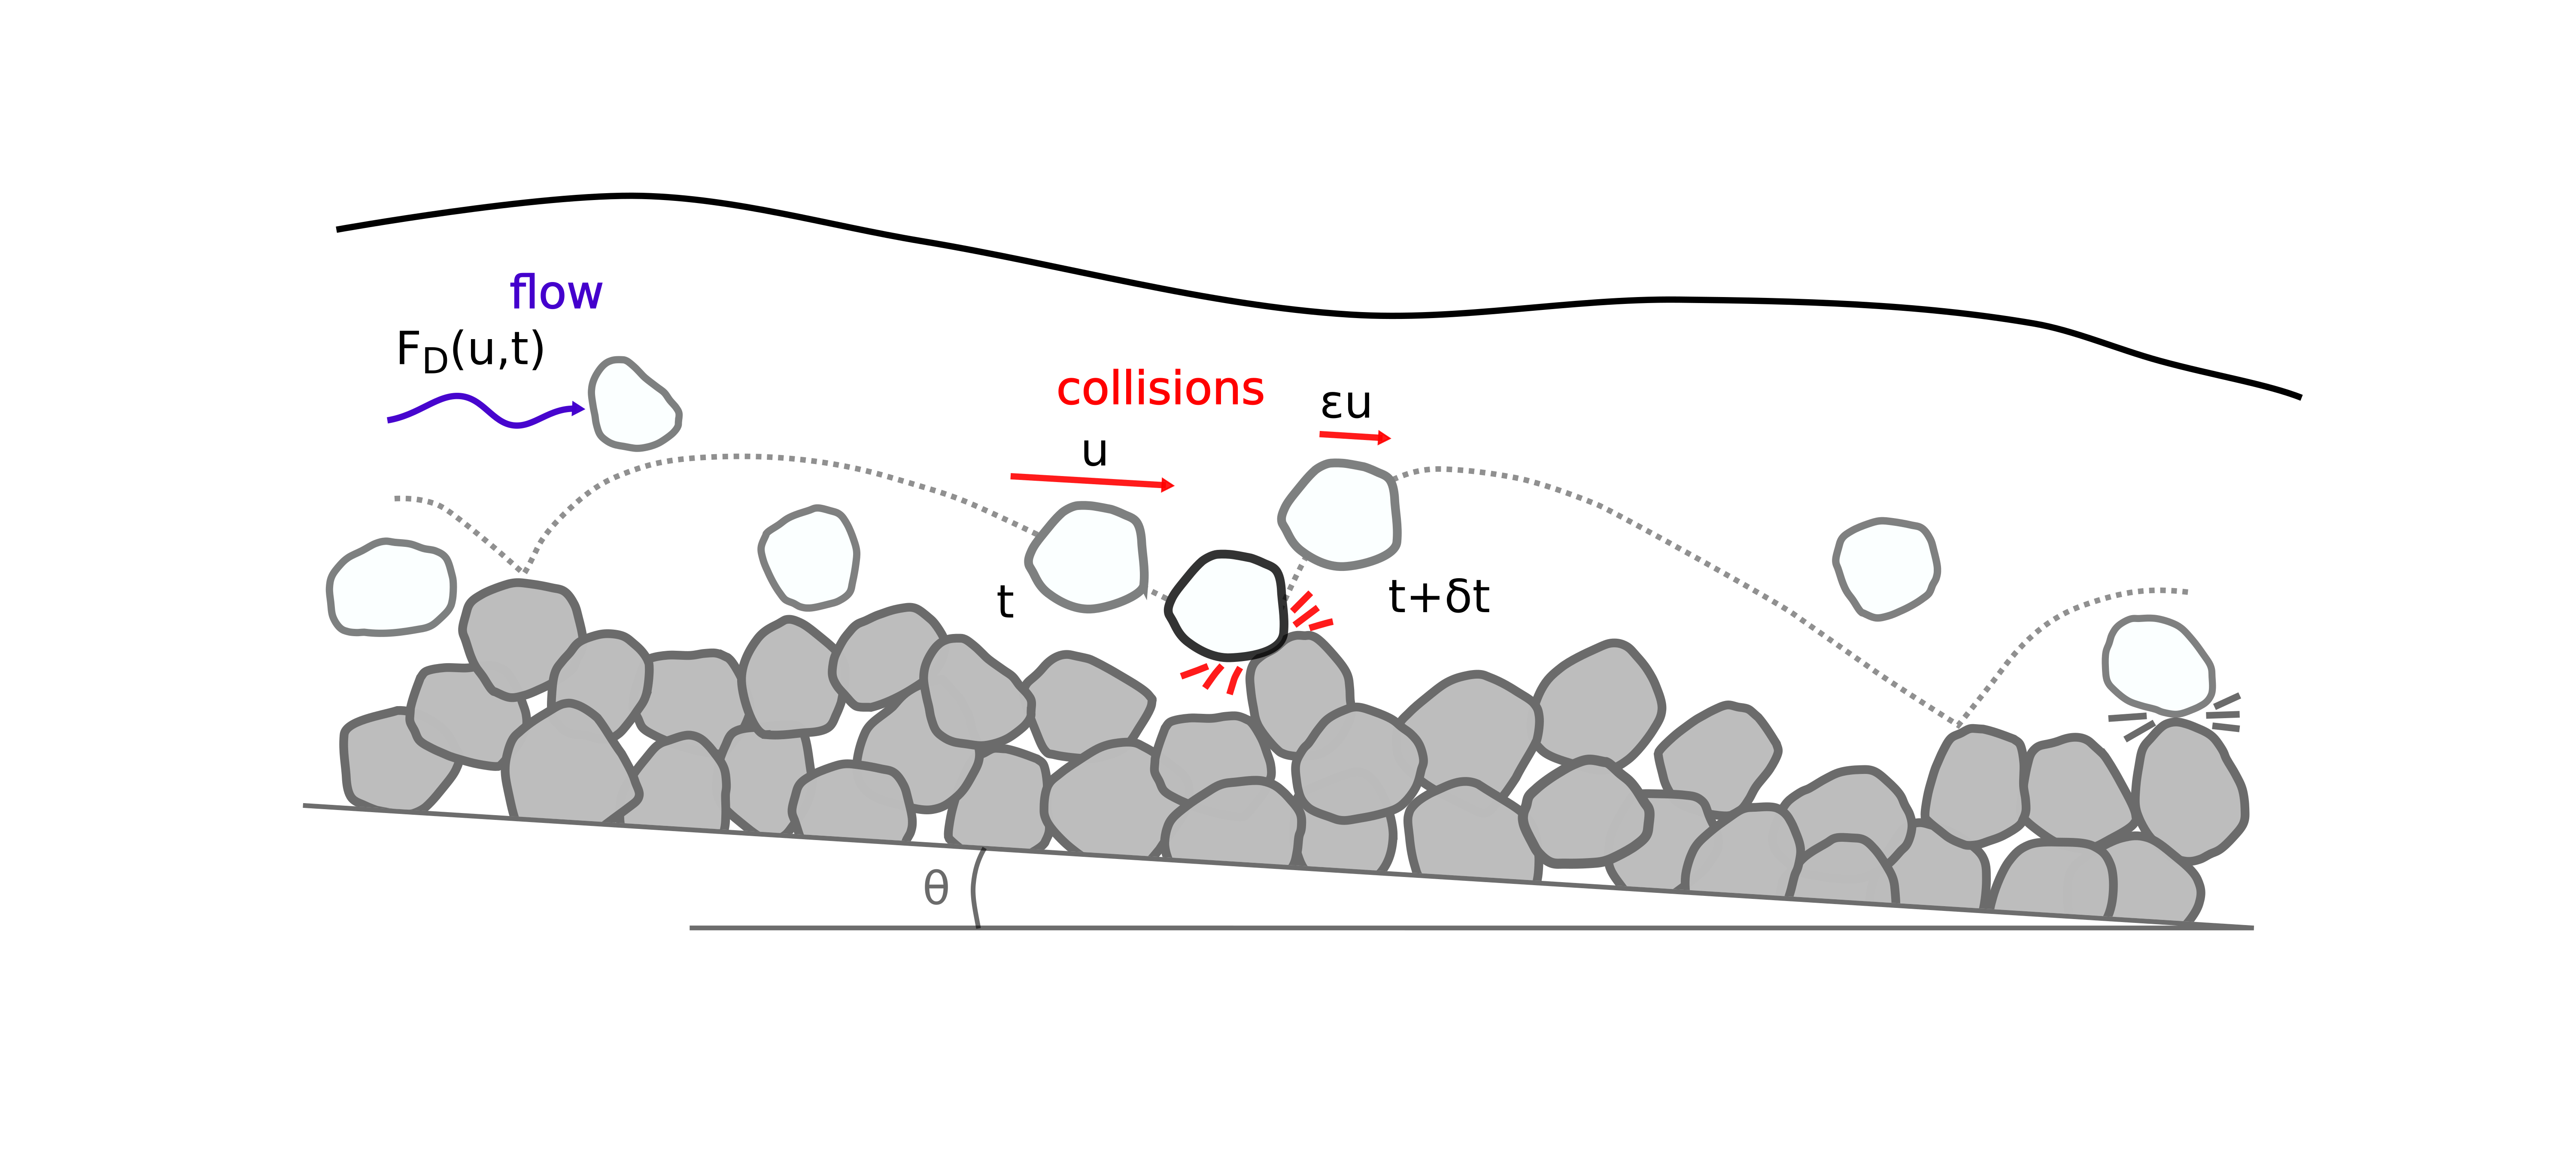
\includegraphics{./figures/ch5/Fig1Concept.png}}
	\caption{Definition sketch of rarefied sediment transport with turbulent fluid drag and particle-bed collision forces. During saltation, pre-collisional streamwise velocities $u$ are transformed to postcollisional velocities $\ve u < u$.}
	\label{fig:fig1}
\end{figure}
Since this quantity combines effects of particle shape and collision geometry and should vary from one collision to the next, we consider that the fraction of streamwise momentum dissipated per collision $\varepsilon$ lies on a statistical distribution $\rho(\varepsilon)$.
Similar ideas are available in the granular physics literature \citep{Serrero2015}.
Further assuming that the number of collisions per unit time is $\nu$ and that the time intervals between subsequent particle-bed collisions are exponentially distributed \citep{Gordon1972}, we write the collision force in the downstream direction as
\be F_C(u,t) = - m u \sum_{k=1}^{N_\nu(t)}(1-\varepsilon_k)\delta(t-\tau_k). \label{eq:col} \ee
Here, $N_\nu(t)$ is the number of collisions in time $t$, the $\tau_k$ ($k=1,2,\dots$) are times at which collisions occur, and the $\varepsilon_k$ are elasticity coefficients characterizing the amount by which each collision slows the particle down.
This collision force is a sequence of random impulses which are proportional to the pre-collisional streamwise momentum. This collision model should be adequate when the contact times between moving and resting particles are small compared to the times between collisions. These conditions are always satisfied for the idealized saltation-type motion depicted in figure \ref{eq:1}.

Fluid forces on a coarse particle in a viscous flow depend on the Reynolds number $\Re_p = d V/\nu$ defined by the particle size $d$, slip velocity $V$ between particle and fluid, and kinematic viscosity $\nu$.
These forces have been calculated analytically from the Navier-Stokes equations for vanishing $\Re_p$ and include acceleration, history, and velocity-dependent drag terms \citep{Hjelmfelt1966, Maxey1983, Auton1987}.
At realistic $\Re_p$ analytical results are limited, so it is standard practice to turn instead to empirical corrections on the small $\Re_p$ formulas \citep{Schmeeckle2007,Mei2006}.
A dominant contribution to the downstream drag force $F_D$ on nearly spherical particles at large $\Re_p$ can be written $F_D = \frac{\pi}{8}
\rho_f d^2 C_D(\Re_p) |V|V$, where $\rho_f$ is the fluid density, $d$ is the particle diameter, $C_D(\Re_p)$ is an empirical drag coefficient, and $V = U-u$ is the slip velocity between the fluid ($U$) and particle ($u$) velocities \citep{Coleman1967, Schmeeckle2007, Dwivedi2012}.
In the present model we set $C_D = \frac{24}{\Re_p}( 1 + 0.194 \Re_p^{0.631})$ \citep{Clift1978,Gonzalez2017} and we do not involve acceleration and history terms for simplicity, although we acknowledge their potential importance for coarse sediment transport \citep{Michaelides1995,Armenio2001,Dalche2015}.

Drag forces have been argued to fluctuate rapidly compared to the inertial response times of coarse sediment grains \citep{Fan2014}.
The magnitude of drag fluctuations has been observed to follow a Gaussian distribution \citep{Hofland2006,Schmeeckle2007,Dwivedi2010,Celik2014}.
Using these ideas, we make two key simplifications of the drag force above.
First, we split the drag $F_D$ into quasi-steady and fluctuating components \citep{Michaelides1997}, and second, we represent drag fluctuations as a Gaussian white noise characterized by a particle diffusivity $D$ \citep{Fan2014,Ancey2014}. 
Defining $\bar{V}$ as a representative slip velocity which we specify more carefully later,  $\bar{C}_D$ as the empirical drag coefficient evaluated at this slip velocity, and $\xi(t)$ as a Gaussian white noise of mean $0$ and variance $1$ \citep{Gardiner1983}, we express the fluid forces as
\be F_D(t) = \frac{\pi}{8}
\rho_f d^2 \bar{C}_D \bar{V}^2 + \sqrt{2 D } \eta(t). \ee
In this drag force \ref{eq:drag} and the collision force \ref{eq:col}, the turbulent fluctuations $\xi(t)$, collision times $\tau_k$, and dissipation coefficients $\varepsilon_k$, can take any values consistent with their distribution and correlation functions. This set of possiblities defines a statistical ensemble.

\subsection{Langevin equation for collisional transport}

With the above forces, we express the Langevin equation $m\dot{u}(t) = F_D(t) + F_C(t)$ for the sediment dynamics as
\be m \dot{u}(t) = \Gamma + \sqrt{2D}\eta(t) - m u(t) \xi_{\nu, \ve}(t). \label{eq:langevin} \ee
This equation replaces the steady friction terms of earlier stocahstic bed load models with an episodic term which provides a more realistic representation of particle-bed collisions during saltation.
It represents a jump-diffusion process \citep{Daly2006} with multiplicative Poisson noise \citep{Dubkov2016,Denisov2009}. 
Collisions introduce ``jumps" in velocity while turbulent generates "diffusion".
The collision term is "multiplicative" in the sense that $u$ multiplies the Poisson noise.
Equations like \ref{eq:langevin} have long been studied in the stochastic physics literature \citep{Hanggi1978,vandenBroek1983}, but solving such equations remains extremely challenging \citep{Luczka1995,Daly2010,Mau2014,Dubkov2019}.
One issue is that multiplicative white noises imply the prescription dilemma of stochastic calculus \citep{Risken1984,Gardiner1983}, meaning \ref{eq:langevin} is not defined without further specifying an integration rule \citep{Suweiss2011}.
Here, the Ito interpretation (lower endpoint integration rule) is the physical choice since the energy dissipated by collisions depends strictly on pre-collisional velocities, not post-collisional.
Given this integration rule, the remaining issues are to obtain the integro-differential equation characterizing the ensemble of velocities defined by \ref{eq:langevin}, and then to solve this equation for the velocity distribution $P(u)$.

\subsection{Chapman-Komogorov equation and particle-bed collision integral}

We derive the equation governing the streamwise velocity distribution $P(u,t)$ from a simple limiting argument in appendix \ref{sec:appendixA}, finding
\be \nu^{-1}\partial_t P(u,t) = - \tilde{\Gamma} \partial_u P(u,t) + \tilde{D} \partial_u^2 P(u,t) + \mathcal{I}_c(u,t). \label{eq:master} \ee
In this equation, we introduced the scaled parameters $\tilde{\Gamma} = \Gamma/(\nu m)$ and $\tilde{D} = D/(\nu m)$. The term
\be \mathcal{I}_c(u,t) = - P(u,t) + \int_0^1 \frac{d\ve}{\ve}P\big(\frac{u}{\ve},t \big) \rho(\ve) \label{eq:colint} \ee
is a ``collision integral" term representing particle-bed collisions.
Equation \ref{eq:master} is a nonlocal extension of the Fokker-Planck equation used in earlier bed load models \citep{Fan2014,Ancey2014}. 
Such equations combining are known as Chapman-Komogorov equations \citep{Gardiner1983}. 
Nonlocality is introduced by the collision integral \ref{eq:colint} which transfers probability from higher pre-collisional velocities $u/\varepsilon$ to lower post-collisional velocities $u$.
This term is analogous to the collision integral of the Boltzmann equation in kinetic theory and granular gases \citep{Duderstadt1971, Brilliantov2004}. Physically, it corresponds to binary collisions between particles having different masses and random resitution coefficients \cite{Serero2015} in the limit that the mass of one particle (here, the particle resting on the bed) goes to infinity. Mathematically, it represents the probability distribution of the product between $\varepsilon$ and $u$ \citep[c.f.][]{Feller1968}.

Owing to its nonlocality, equation \ref{eq:master} does not admit analytical solutions as is, so we make one further approximation.
We assume the distribution of dissipation coefficients $\rho(\varepsilon)$ is sharply peaked at some most common (mode) value $\varepsilon'$. This allows for a Kramers-Moyal type expansion of the particle-bed collision integral \citep{Gardiner1983}.
Expanding all terms in the integrand except $\rho(\varepsilon)$ provides
\be \mathcal{I}_c(u,t) = -P(u,t) + \frac{1}{\varepsilon'}P\big(\frac{u}{\ve'},t \big) + \sum_{k=1}^\infty \frac{\alpha_k }{k!}(\ve - \ve')^k \Big[\frac{1}{\ve}P\big(\frac{u}{\ve}\big)\Big]^{(k)}\Big|_{\ve=\ve'},\label{eq:expansion}\ee
where the $\alpha_k = \int_0^1 d\ve \rho(\ve) (\ve-\ve')^k $ are the central moments of $\ve$ around the mode elasticity $\ve'$ and the superscript $(k)$ denotes the $k$th derivative.
In what follows, we drop all but the first two terms to obtain the leading order contribution of particle-bed collisions to the velocity distribution. Higher orders could always be included later by perturbation theory. We solve the resulting approximate equation in steady-state, when $\partial P(u,t)/\partial t = 0$. Scaling the time in Equation \ref{eq:master}, we can see this solution will be a good approximation to the time-dependent problem when particle motions generally survive multiple collisions.

\section{Results}
\label{sec:results}

\subsection{Derivation of the bedload velocity distribution}
\label{sec:solution}
Hereafter we drop the prime on the most common streamwise restitution coefficient $\ve'$. With the truncation to two terms, equation \ref{eq:master} gives 
\be 0 = -\tilde{\Gamma}\partial_u P(u) + \tilde{D}\partial_u^2 P(u) -P(u) + \frac{1}{\ve} P\big(\frac{u}{\ve}\big),\label{eq:governer} \ee
which is now a non-local ordinary differential equation. Such equations have seen some attention in the mathematics literature, where they are called pantograph equations \citep{Hall1970,Zaidi2015,Bhalekar2017} for their relationship to a current collection device used on electric trains \citep{Ockendon1971}.
In the appendix we solve equation \ref{eq:governer} using Laplace transforms, providing
\begin{multline} P(u) = \frac{\theta(-u)}{K_+}\sum_{l=0}^\infty \frac{\ve^{-l}e^{\lambda_+\ve^{-l}u}}{\prod_{m=1}^l(-\tilde{D} \lambda_+^2 \ve^{-2m} + \tilde{\Gamma} \lambda_+ \ve^{-m} + 1) } 
	\\+ \frac{\theta(u)}{K_-}\sum_{l=0}^\infty \frac{\ve^{-l}e^{\lambda_-\ve^{-l}u}}{\prod_{m=1}^l(-d \lambda_-^2 \ve^{-2m} + \gamma \lambda_- \ve^{-m} + 1) } \label{eq:steadystate}. \end{multline}
The factors $\lambda_\pm$ are defined in the appendix; they are proportional to $\tilde{\Gamma}/\tilde{D}$. 
The normalization factors are $K_\pm$ are 
\be K_\pm = d(\lambda_+-\lambda_-)\prod_{l=1}^\infty (-d\lambda_\pm^2 \ve^{2l} + \gamma \lambda_\pm \ve^{l} + 1). \ee
Although this velocity distribution appears quite complicated, one can verify that this is a normalized probability distribution which has very simple limiting behaviors as the most common dissipation coefficient $\ve$ approaches fully elastic ($\ve=1$) and inelastic ($\ve = 0$) values.

It is rather simple to derive the moments of this probability distribution by multiplying \ref{eq:governer} by $u$, integrating, and then solving the resulting moment evolution equations \citep[c.f.][]{Cox1965}.
The first moment is
\be \langle u \rangle = \frac{\Gamma}{\nu(1-\ve)} = \frac{\gamma}{1-\ve},\ee
which is scales weakly with the mean fluid drag and sharply with the rate and typical elasticity of collisions.
The second moment is
\be \langle u^2 \rangle = 2 \frac{d + \gamma \langle u \rangle}{1-\ve^2}, \ee
leading to the velocity variance ($\sigma_u^2 = \bra u^2 \ket - \bra u \ket ^2 $)
\be \sigma_u = \sqrt{\frac{2 d + \gamma^2}{1-\ve^2}}.\ee
This equation demonstrates that velocity fluctuations originate from both the steady and fluctuating components of the flow forces, yet the variance is linear in these factors and is therefore relatively insensitive to them. In contrast, velocity fluctuations depend sharply on the parameters representing particle-bed collisions.

Figure \ref{fig:fig2} depicts velocity characteristics for different realizations of the fluid and collisional forces.
\begin{figure}
	\centerline{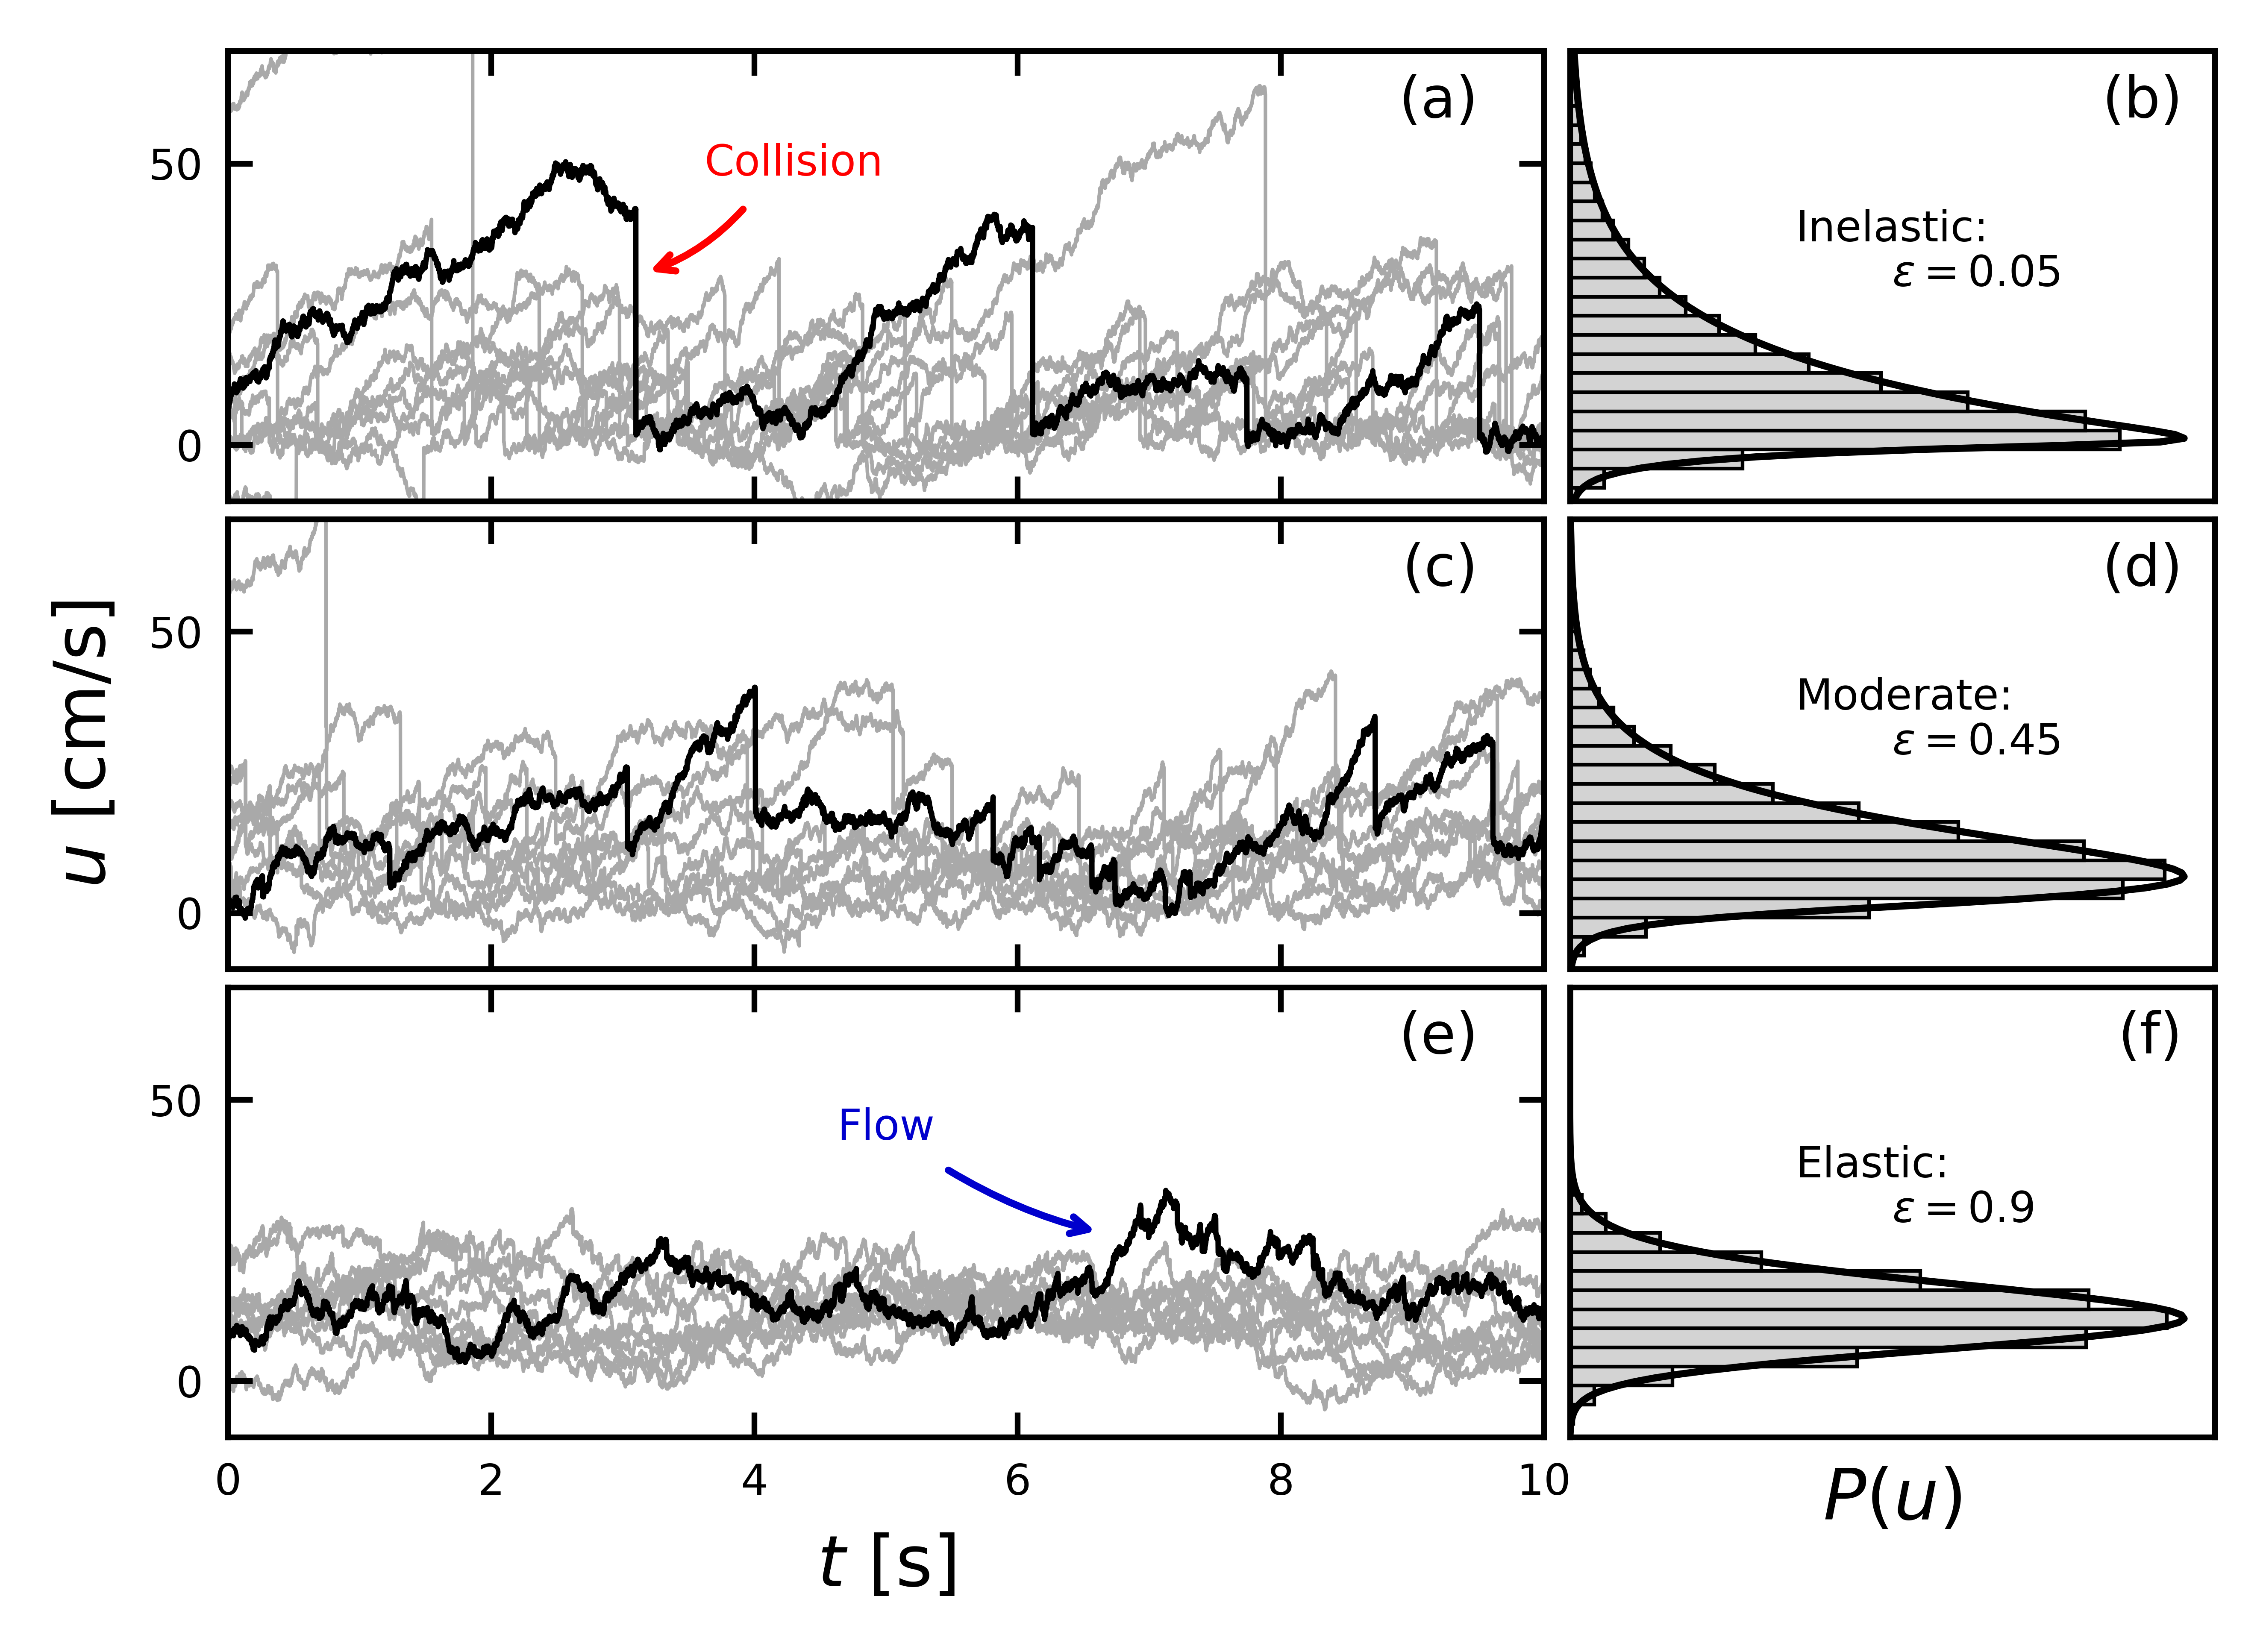
\includegraphics{./figures/ch5/Fig2pdfs.png}}
	\caption{Left panels show velocity realizations as gray traces. Velocities are calculated from Monte Carlo simulations. Individual realizations are singled out as black traces. Particle-bed collisions imply sudden downward-velocity jumps. Flow forces generate fluctuating positive accelerations between collisions. Right panels show simulated histograms of particle velocities and exact solutions from equation \ref{eq:steadystate}.}
	\label{fig:fig2}
\end{figure}
We can see an apparent transition from exponential-like to Gaussian-like velocity distributions as typical collisions vary from more inelastic ($\ve \rightarrow 0$) to more elastic ($\ve \rightarrow 1$). In between, the full distribution \ref{eq:steadystate} resembles a Gamma distribution, although it is not a Gamma distribution.


\subsection{Exponential and Gaussian regimes: limits to earlier work}
\label{sec:modelcomparison}

In fact, the apparent transition in figure \ref{fig:fig2} can be made rigorous: despite its complex appearance, simple Gaussian and exponential distributions appear as rigorous mathematical limits of equation \ref{eq:steadystate}. When particle-bed collisions are completely inelastic, \ref{eq:steadystate} becomes an exponential distribution, and when they are completely elastic, \ref{eq:steadystate} becomes Gaussian. Figure \ref{fig:fig3} demonstrates more closely the approach of the distribution toward these limits.
\begin{figure}
	\centerline{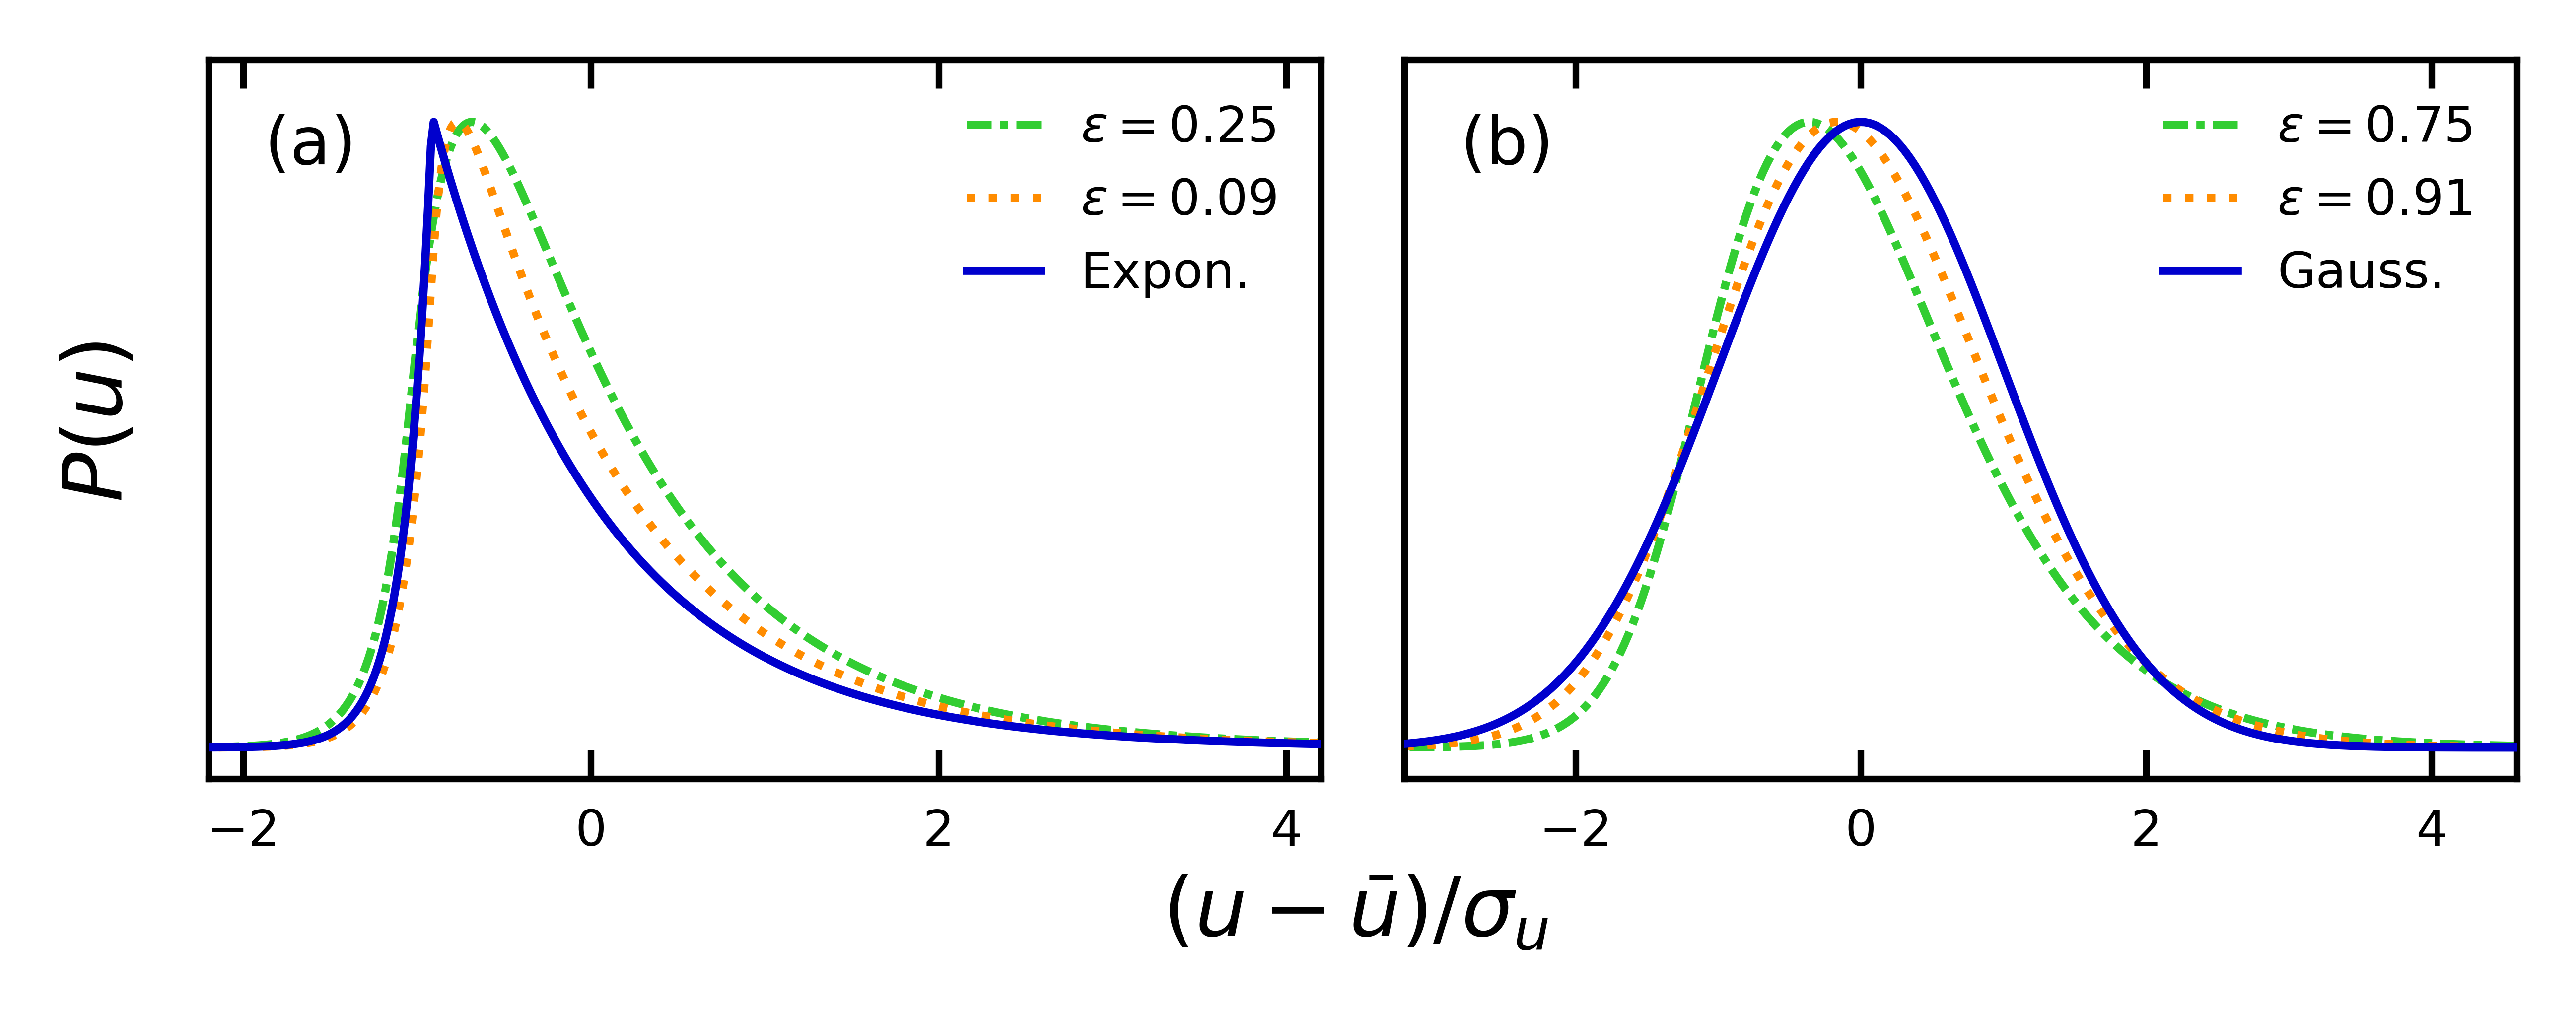
\includegraphics{./figures/ch5/Fig3asymptotic.png}}
	\caption{The particle velocity distribution approaches an exponential distribution in (a) as particle-bed collisions become extremely elastic ($\ve \rightarrow 1$), and it approaches a Gaussian in (b) as they become extremely inelastic ($\ve \rightarrow 0$). On the abscissa, the mean sediment velocity is standardized by its mean $\bar{u}$ and standard deviation $\sigma_u$. }
	\label{fig:fig3}
\end{figure}

The exponential limit of \ref{eq:steadystate} as $\ve \rightarrow 0$ is rather easy to see. Taking $\ve \rightarrow 0 $ in \ref{eq:steadystate}, all terms in the series except for that with $l=0$ become exponentially small, leaving behind the same two-sided exponential distribution derived by \cite{Fan2014} up to notational differences:
\be P(u) = \frac{d}{\sqrt{\gamma^2 + 4d}}e^{\frac{\gamma u }{2 d} - \frac{\sqrt{\gamma^2 + 4 d}|u|}{2d}}. \ee
Thus, for bed load transport conditions with typically very inelastic particle-bed collisions, we can expect exponential-like velocities and large deviations from a Gaussian behavior.

The Gaussian limit as $\ve \rightarrow 1$ of \ref{eq:steadystate} is more difficult to evaluate. The challenge is that the statistical moments \ref{eq:mean} and \ref{eq:2ndmom} diverge at the same time as the denominator factors of the distribution \ref{eq:steadystate}. In appendix \ref{sec:appendixB} we return instead to the original equation \ref{eq:governer} to evaluate this elastic limit, obtaining
\be P(u) = \frac{1}{\sqrt{2\pi\sigma_u^2}}e^{-\frac{(u-\bar{u})^2}{2\sigma_u^2}}. \label{eq:gaussian}\ee
This result is identical to the velocity distribution derived by \citet{Ancey2014}, up to notation.

\subsection{Comparison with experimental data}
\label{sec:experimentcomparison}

Now we compare the analytical distribution \ref{eq:steadystate} with the available experimental data.
Upfront, we point out that the distribution above has free parameters and this is only a proof of concept that the velocity distribution is capable of fitting the available experimental data; it is not a proof that this is the underlying mechanism for these data blahblahblah that was a good writing day.


\begin{table}
	\begin{center}
		\def~{\hphantom{0}}
		\begin{tabular}{lccc}
			$a/d$  & $M=4$   &   $M=8$ & Callan  \\[3pt]
			0.1   & 1.56905 & ~~1.56~ & 1.56904\\
			0.3   & 1.50484 & ~~1.504 & 1.50484\\
			0.55  & 1.39128 & ~~1.391 & 1.39131\\
			0.7   & 1.32281 & ~10.322 & 1.32288\\
			0.913 & 1.34479 & 100.351 & 1.35185\\
		\end{tabular}
		\caption{Values of $kd$ at which trapped modes occur when $\rho(\theta)=a$.}
		\label{tab:kd}
	\end{center}
\end{table}


\begin{figure}
	\centerline{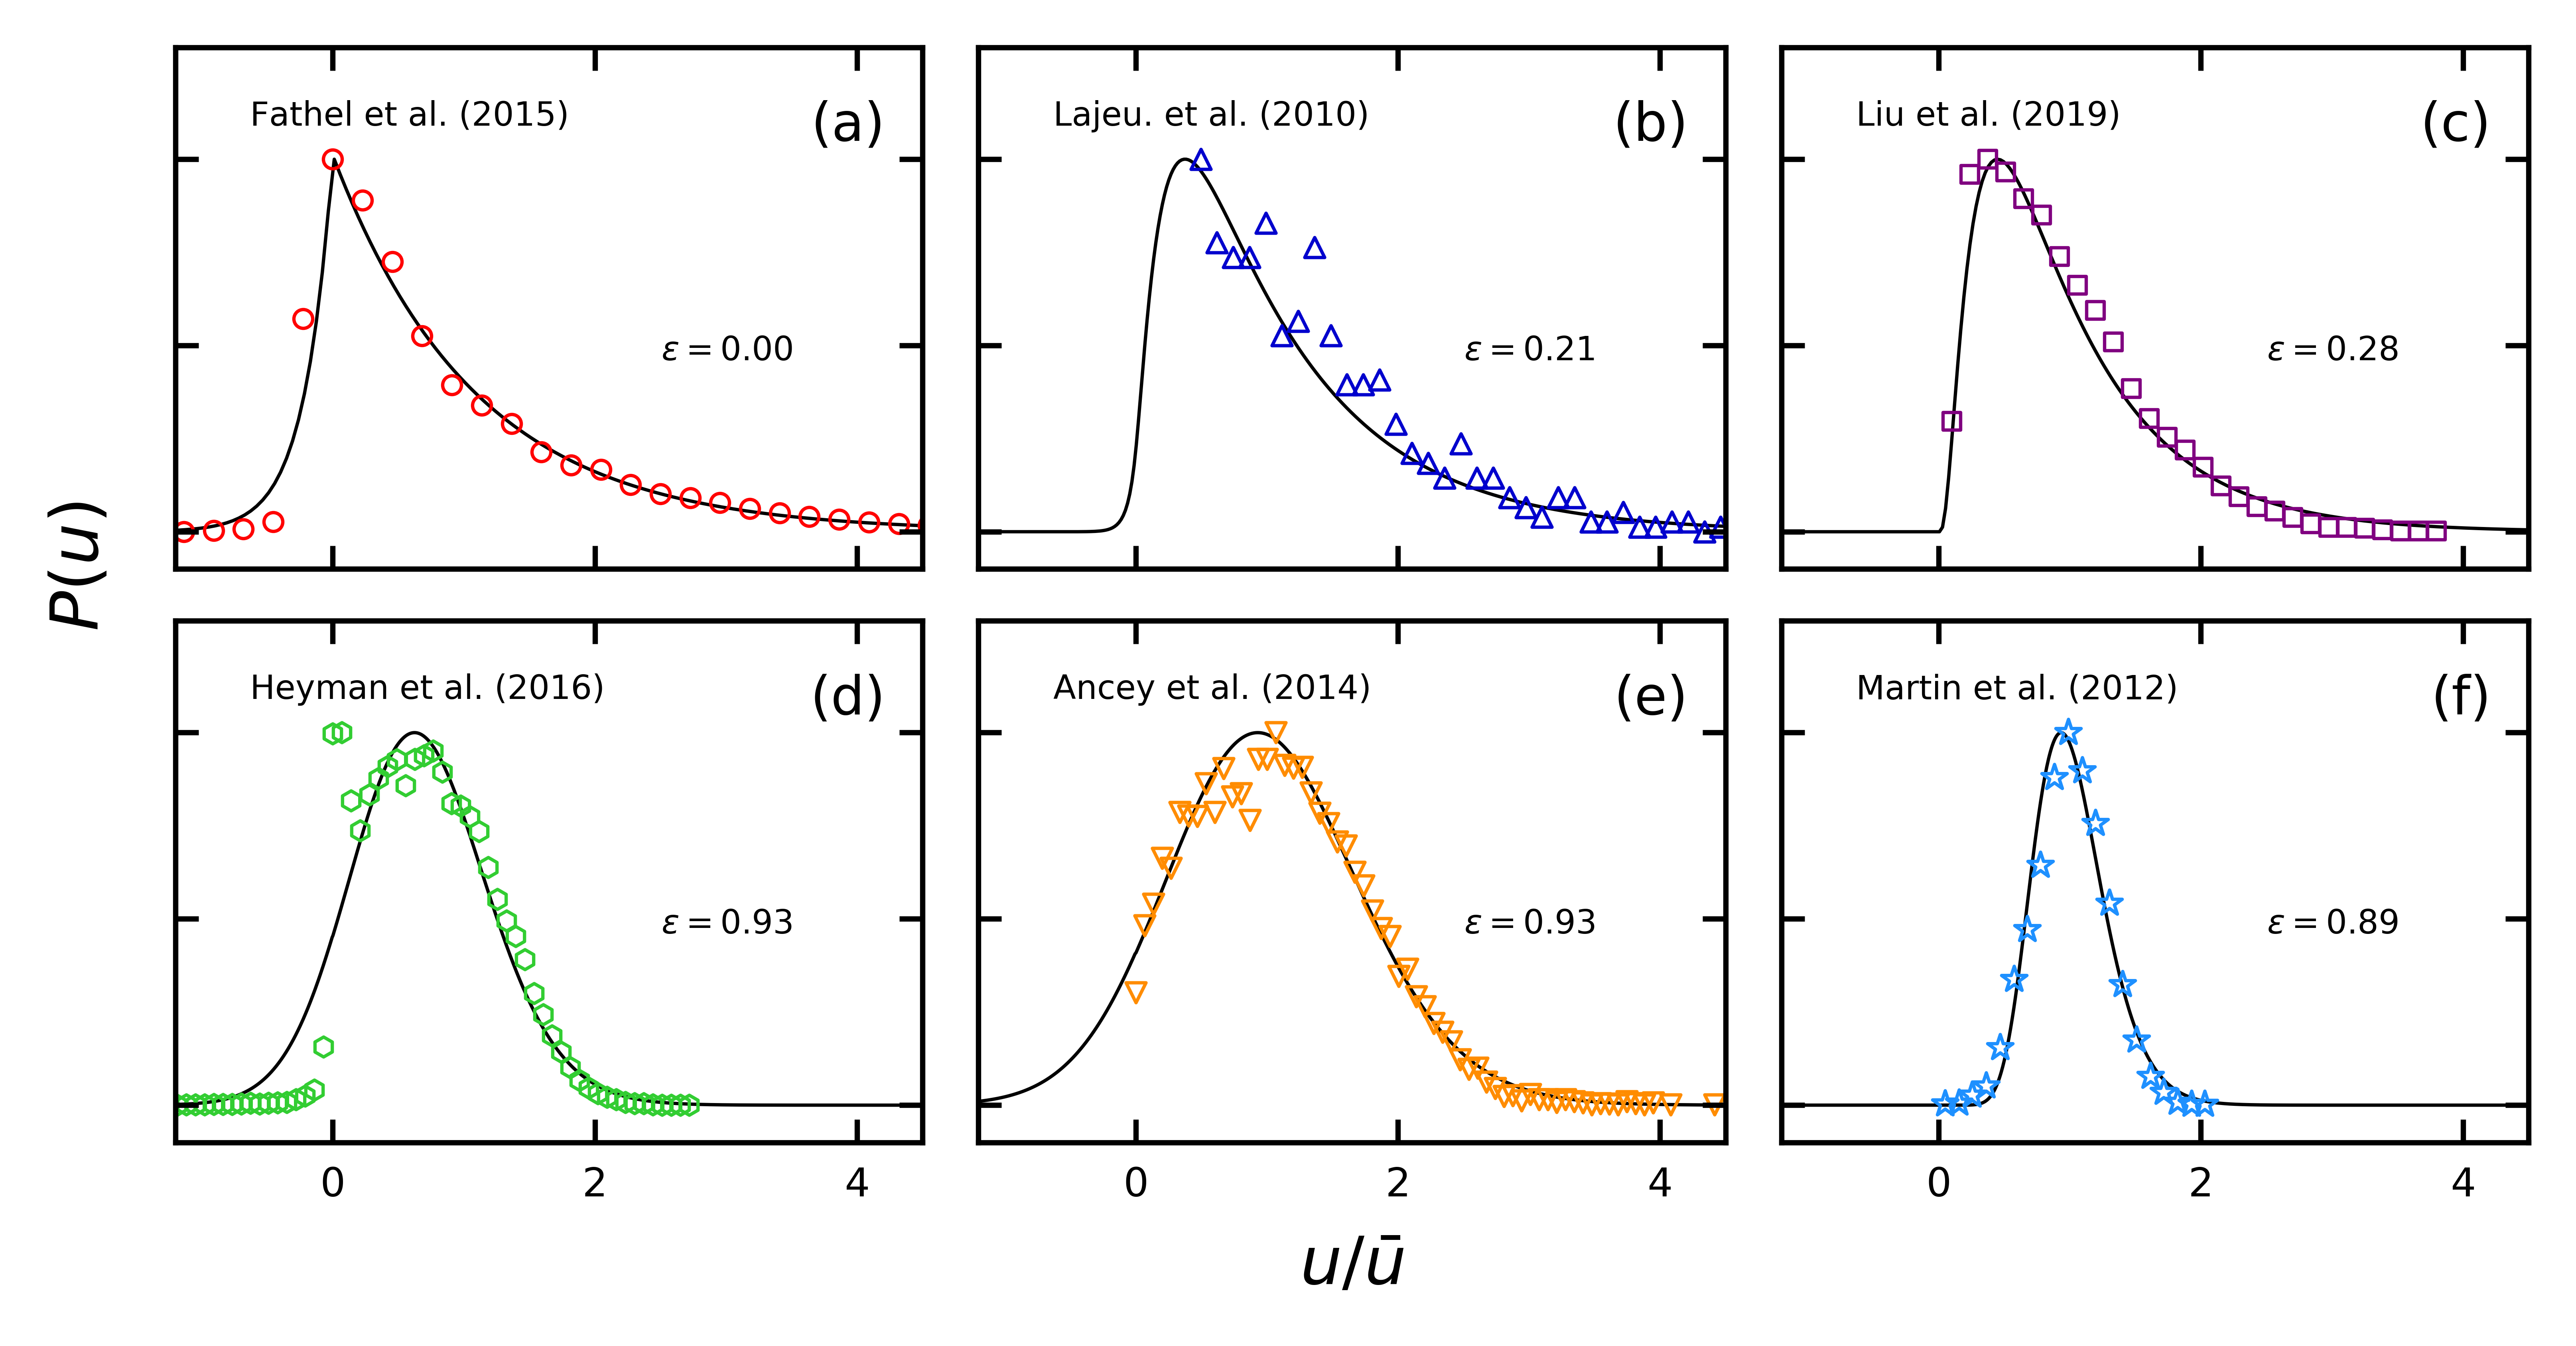
\includegraphics{./figures/ch5/Fig4expComparison.png}}
	\caption{The features of the four possible modes corresponding to
		(\textit{a}) periodic\protect\\ and (\textit{b}) half-periodic solutions.}
	\label{fig:fig4}
\end{figure}


\section{Discussion}
\label{sec:discussion}

Here, I developed a Langevin description of bed load sediment transport which includes episodic collisions between particles and the bed.
The model relates the shape of the instantaneous streamwise particle velocity distribution to the elasticity of particle-bed collisions,
generalizes earlier approaches available in the literature which did not treat episodic collisions \citep{Ancey2014,Fan2014}, and provides a new physical explanation for the different streamwise sediment velocity distributions resolved in experiments.
Although in reality, the turbulent forces on moving sediment particles vary in a complex spatio-temporal way, we have approximated the fluid forces on bed load particles as spatially uniform Gaussian white noise. Even though the non-Gaussian aspects of fluid turbulence certainly do impact sediment entrainment \citep{Coleman2019,Celik2014}, this flow model appears more or less justified since sediment transport experiments provide similar velocity distributions regardless of whether the flow is viscous or turbulent \citep{Lajeunesse2010, Charru2004}, and since particle relaxation times are typically long compared to the timescales of turbulent fluctuations \citep{Hofland2006,Schmeeckle2007,Nakagawa1981}.
We modelled particle-bed collision forces as a sequence of instantaneous impulses where the intervals between successive collisions were characterized as exponential random variables. The effect of each collision on the streamwise particle velocities was parameterized by a restitution-like coefficient.
Although such approximate descriptions of particle-particle collisions are common in the theory of granular gases, the setting here is somewhat different than grains in air. Because particles within a viscous flow in general interact at a distance, we should expect the collision model will become poor when the time between subsequent collisions becomes small. Therefore, although the model seems appropriate for saltation, it should be critically examined for ``reptation", when the times between subsequent particle-bed collisions are short. Of course, more realistic flow and collision forces could always be incorporated into Langevin equations for bed load transport, although these might require numerical methods for their solution. The theory of granular gases provides some indication of the types of more nuanced collision models which are possible \citep{Brilliantov2004,other..}.

Sediment transport experiments reveal correlations between particle size and the shape of the bed load velocity distribution.
Experiments with smaller particles tend to give exponential distributions, and those with larger particles give Gaussian distributions.
In fluid dynamics, the dissipation characteristics of particle-particle collisions in viscous flows are known to depend on the particle size and approach velocity through the Stokes number. 
In kinetic theory, it is known that gases of ideal elastic particles generate Gaussian (Boltzmann) velocity distributions, while gases of inelastic grains generate non-Gaussian distributions \citep{Chapman1970,Brilliantov2004}.
Taken together, these ideas suggest that we might relate the shape of the particle velocity distribution to particle size.
We can estimate typical Stokes numbers of colliding bed load particles in experiments as $...$, using with the flow shear velocity and mean streamwise sediment velocity to calculate $V$. Estimating in this way, transport experiments with exponential velocities have $St \sim 1-10$, those with neither exponential nor Gaussian velocities have $St \sim 10-100$, and those with Gaussian velocities have $St > 100$.
In experiments relating restitution coefficient to Stokes number for idealized collisions, restitution coefficients vary sharply from $0$ to $1$ as $St$ ranges from $1$ to $500$ \cite{Marshall2001,Joseph2001,Yang2006}.
Although collision geometry and grain shape certainly complicate the narrative, these values of $St$ are consistent with our model conclusion that the shape of the particle velocity depends on the elasticity of collisions.

In real channels, grain sizes often span a wide range. A major implication of the dependence of the shape of the particle velocity distribution on grain size is that different grain sizes in a mixture will impart distinct fluctuation signatures to the overall bulk transport rate. Even in the absence of sorting effects and differential mobility, smaller grains can be expected to carry more control over the largest fluctuations in the overall transport rate, since their velocity distributions have wider tails. 

\subsection{Implications for landscape evolution}

Many phenomena of landscape evolution depend on the velocities of individual grains.
The erosion rates of bedrock rivers are for example parameterized by the impact velocities of individual sediment grains against the bedrock surface \citep{Skylar2004,Tingian,Turowski2020}, on which they have a sensitive nonlinear dependence.
It is not much of a stretch to imagine that bedrock erosion could be dominated by the largest impact velocities that originate from the extreme tail of the bedload velocity distribution. Here, we have shown that the weight of this tail depends sensitively on the dissipation characteristics of particle-bed collisions, suggesting that another feedback, that between dissipation and ... may be at play in the evolution of bedrock canyons.

\subsection{Analogies to hillslope and wind-driven transport}

It has long been recognized, probably since \citet{Bagnold1941} and certainly today \citep{}, that there are deep analogies between tranpsort phenomena in air and water.
In an ideal perspective, we might imagine writing the governing equations for transport in water as a function of the fluid viscosity, then tuning the viscosity between air and water to obtain a description applying to both spheres.


For example, in a mixture of small and large grains, neglecting any sorting effects whereby the mobility of small grains is contingent on the mobility of the large grains, small grains will have exponential velocities with relatively wide fluctuations, while large grains will have Gaussian velocities with relatively narrow fluctuations. Considering the over-all flux then as the number of moving particles times their velocities, transport fluctuations



aeolean transport extension maybe
particle size distributions - interesting implications
connection to computational physics approach
connection to the stochastic description of the flux





\section{Conclusion}
We have demonstrated that particle-bed collisions control the shape of the particle velocity distribution.  
\label{sec:conclusion}

%%!TEX root = ../diss.tex

\chapter{Summary and future work}
\label{ch:conc}

This thesis has described bedload transport from the statistical physics of individual grains.
The work has improved upon earlier descriptions.
It describes the movements of grains along a wider range of timescales than before, highlights Langevin equations, master equations, and random walks as the common threads of stochastic sediment transport modelling, and provides more realistic descriptions of bedload transport. In particular, I have
\begin{enumerate}
	\item developed the linkage between sediment flux probability distributions and individual particle trajectories (ch. \ref{ch:flux}), 
	\item described particle trajectories alternating through motion and rest with fluctuating velocities (ch. \ref{ch:flux}),
	\item evaluated the control of bed elevation changes over sediment transport rates (ch. \ref{ch:ch3}),
	\item characterized how long particles can remain buried within the sedimentary bed (ch. \ref{ch:ch3}),
	\item incorporated the process of sediment burial in a description of downstream particle movement (ch. \ref{ch:downDiff}), and
	\item formulated the velocity distributions of sediment particles including episodic particle-bed collisions (ch. \ref{ch:langevin}).
\end{enumerate}
These developments improve understanding of sediment transport in streams.

\section{Overall methodology of the thesis}

\subsection{Langevin and master equations}

The overarching strategy in all of these developments has been to identify control and response variables, represent control variables by idealized noises (entrainment and deposition events, particle burial events, turbulent forces, or particle-bed collisions), and then formulate dynamical equations relating the response variables to these stochastic control variables.
This strategy phrases sedimentary dynamics in terms of Langevin-like equations, stochastic analogues of Newton's $F=ma$, where the acceleration $a$ is swapped for the response variable of interest in the problem and the force $F$ is a stochastic combination of the control variables. 

Once the stochastic dynamical equations were written for a given problem, its solutions were averaged over realizations of the control variables to produce a master equation, an integro-differential equation governing the probability distributions of the response variables.

The solutions of the master equation in a given problem produce the probability distribution for the response variable of interest, which in the thesis has included at different points the bedload particle position (chs. \ref{ch:flux} and \ref{ch:downDiff}), the particle velocity (ch. \ref{ch:langevin}), the bed elevation (ch. \ref{ch:ch3}), and the sediment transport rate (ch. \ref{ch:flux}).
The same stochastic strategy should be applicable to a wide range of problems in geomorphology where phenomena can built up from component parts with apparently noisy characteristics.


\subsection{Idealized noises and their combinations}

A major challenge in this research is that only a handful of noises in statistical physics are comprehensively understood \citep{Horsthemke1984}, so the available options in stochastic modelling are constrained.
The noises used in this thesis include white Gaussian, Poisson, and dichotomous noises, representing erratic fluctuations, sequences of spikes, and random switches respectively \citep{VanDenBroeck1983}.
Turbulence was described using Gaussian noise, while instantaneous steps, particle arrivals to a control surface, and particle-bed collisions were described with Poisson noise. Alternation between motion and rest was represented with dichotomous noise.
Whenever these processes acted in combination, the dynamical equations describing the response variable included multiple sources of idealized noise as required.
This inclusion of multiple noise sources has not yet to my knowledge been pursued in any earlier stochastic models of sediment transport.

River science offers no guarantee that these idealized white noises which we happen to understand best are sufficient to describe its phenomena.
White noises are an idealization which is probably never realized in nature \citep{Gardiner1983,Kubo1978}.
In contrast, colored noises in which fluctuations have favoured frequencies are well-known to occur in many fluid and granular physics phenomena, most famously in context of fluid turbulence \citep{Kolmogorov1941,Nikora2000} and granular collapse \citep{Bak1987,Jensen1998}.
In river science, many phenomena exhibit colored spectra, like the size distributions of bedforms \citep{Nikora1997,Guala2014}, the fluid forces on bed particles \citep{Dwivedi2011, Amir2014}, the roughness characteristics of gravel beds \citep{Aberle2006,Singh2012}, and sediment flux timeseries \citep{Dhont2018,Chartrand2021}.
It will be problematic if these phenomena require colored noise for their description. Dynamical equations driven by colored noise can be extremely challenging to solve \citep{Hanggi1978,Luczka2005,Hanggi2007}.
Even if white noise models like those developed in this thesis are not exactly accurate, they remain necessary as a basis for comparison when formulating and solving colored noise models \citep{Fox1986,Moss1989}.

\section{Key contributions}

\subsection{Calculation of the probability distribution of the sediment flux from micromechanics of particle transport}

The first major contribution of this thesis is in chapter \ref{ch:flux}. Here, I formulated the probability distribution of the sediment flux from the trajectories of individual particles moving downstream. This work unifies the sediment trajectory models originating from Einstein (secs. \ref{sec:einwalk}-\ref{sec:lisle}) with the renewal approach to calculate the sediment flux (sec. \ref{sec:renewal}).
The striking feature of this formulation is that, as a result of the particle dynamics, the mean bedload flux becomes scale-dependent, whereby the expected magnitude of the flux depends on the time-period over which it is observed.

\citet{Ballio2018} explained that scale-dependence originates from individual particle trajectories, but this had not been described in a mathematical model until now.
Descriptions of the mean sediment flux from the movement characteristics of individual grains have existed now for a long time (sec. \ref{sec:einflux}), and an emerging body of research has producing the full probability distribution of the flux, but without referencing individual movement characteristics (secs. \ref{sec:birthdeath}-\ref{sec:renewal}). 
This work unifies these two research themes and presents a statistical mechanics formulation of bed load sediment transport based on individual particle trajectories.

\subsection{Inclusion of velocity fluctuations into Einstein's model of individual particle trajectories}

Second, in chapter \ref{ch:flux} I developed the first analytical description of sediment trajectories through motion and rest including velocity fluctuations within the motion state.
Einstein originally formulated sediment transport as a sequence of instantaenous steps and rests (sec. \ref{sec:einwalk}), and this was later improved to include the duration of motion (sec. \ref{sec:lisle}).
Until this thesis, movement velocities in analytical models were considered constant which contrasts with reality. 
Although some numerical models have described motion/rest cycles with velocity fluctuations \citep{Fan2016,Bialik2012,Schmeeckle2014}, they had not resolved the novel three-range diffusion characteristics these dynamics imply.

This description predicts multiple-range diffusion across local, intermediate, and global scales as a result of particle velocity fluctuations within the motion state; it introduces a dimensionless Peclet number as an important characteristic of bedload sediment transport; and it relates the timescales at which transitions between local, intermediate, and global timescales occur to the movement characteristics of individual grains.
These developments constitute a new understanding of bedload movement across its timescales.

\subsection{Quantification of the control of bed elevation fluctuations over sediment transport fluctuations}

Third, chapter \ref{ch:ch3} modified the birth-death description of bedload transport (sec. \ref{sec:birthdeath}) to include feedbacks between the local bed elevation and the entrainment and deposition rates.
This allowed for a mathematical investigation of (1) how bed elevation changes affect sediment transport rates and (2) how bed elevation changes control the residence times of particles buried in the bed.
Sediment transport fluctuations have come under increasing scrutiny with the resurgence of stochastic modelling in sediment transport, while the burial times of particles are crucial for using sediment tracers to predict sediment transport.
Earlier birth-death models had generally considered that entrainment and deposition rates of particles remain constant even though these processes imply bed degradation and aggradation respectively, which are known to modify the entrainment and deposition rates in a negative feedback.

This work demonstrates that this negative feedback buffers bedload transport fluctuations whenever collective entrainment occurs, meaning the magnitude of bedload transport fluctuations depends on the rate of bed elevation change. The residence times of buried particles are random variables that lie on heavy-tailed power-law distributions. These distributions allow for arbitrarily long resting times, which poses challenging implications for researchers attempting to predict the downstream sediment flux in applications by tracking sediment tracer particles. 

\subsection{Characterization of how sediment burial affects the downstream transport of sediment particles}

Fourth, chapter \ref{ch:downDiff} presenting a model of sediment trajectories through motion, rest, and burial, describing sediment transport across local, intermediate, global, and geomorphic ranges (), and producing new understanding of how exactly the distinct spreading characteristics of particles within each of these ranges arise \citep[e.g][]{Pretzlav2021}.

Until this work, the mechanisms which produce the different spreading rates of particles across the scaling ranges identified by Nikora and coworkers had been uncertain for several decades, and earlier works had included what were believed to be the required features without describing three or more scaling ranges. 
The work ultimately demonstrates that many approaches to describe individual particle motions are reformulations of the continuous time random walk formalism from physics, indicating underlying unity within a diverse body of research and bringing powerful tools from statistical physics to the sediment transport problem.

\subsection{Description of how particle-bed collisions control movement velocities of grains}

Finally, chapter \ref{ch:langevin} displayed a new theoretical model of individual grains saltating downstream in a turbulent flow through a sequence of particle-bed collisions.
This work provides the first comprehensive description of all bedload velocity distributions observed in experiments (sec. \ref{sec:langexperimentcomparison}), while earlier works had described only particular end-member distributions (sec. \ref{sec:langevin}).

\section{Limitations and future research directions}

This thesis has produced new understanding of how to describe bedload transport using statistical physics, but its approach has many limitations deserving of future research attention.
In some cases these are specific to the models produced in the thesis, but in others, they are shared in common with a majority of models in the stochastic sediment transport research paradigm \citep{Ancey2020,Furbish2021a}.

\subsection{Landscape dynamics and channel morphology}

The first limitation concerns the assumption, implicit in every chapter of this thesis, that sediment transport characteristics are steady and uniform in time and space.
This assumption contrasts with conditions in real gravel-bed rivers, where riffles, bars, and steps coordinate the movements of individual grains \citep{Ashmore1998,McDowell2020}, sediment is supplied in episodic bursts from mass movements \citep{Benda1990, Muller2018}, woody debris coordinates sediment movement \citep{Eaton2012,Reid2019}, and variable flow conditions modify bed texture and sediment availability \citep{Mao2012,Phillips2018}.

To date, very little work has concentrated on stochastic sediment transport models in unsteady conditions \citep[e.g.][]{Bohorquez2016}.
The most obvious scheme to address unsteadiness is to introduce time and space dependence to movement velocities, diffusivities, or entrainment and deposition rates, but how exactly one should express these rates in terms of time and space is a matter for speculation, and would be contingent on a given context given our limited understanding of how these parameters relate to the flow hydraulics \citep[e.g.][]{Heyman2016}.

Future studies might investigate in more depth the linkage between flow hydraulics, the geometric arrangement of grains on the bed, and the bed topography with the entrainment and deposition rates of individual particles to develop the foundational knowledge to incorporate temporally or spatially variable flow and sedimentary conditions into stochastic models of sediment transport.

\subsection{Grain size distributions}

The second major limitation of this work concerns grain size.
In actuality, sediments in rivers spans a range of sizes, and differential mobility based on particle size produces spatial sorting, both vertically as in bed armoring \citep{Parker1982,Wilcock1989,Aberle2006}, and laterally as patch, particle cluster, or riffle development \citep{Nelson2014,Venditti2017}.

There have been a few works on stochastic modelling of sediment transport with multiple grain sizes \citep{Sun2000,Parker2000}, but these approaches are not spatially distributed, so there is as yet no stochastic method to understand sorting processes. 

Future studies should revisit the stochastic framework applied to multiple grain sizes. Simplified experimental geometries based on bimodal sediment beds \citep[e.g.][]{Houssais2012} would be a great context to revisit these issues. Extending the motion-rest model of chapter \ref{ch:ch3} to two grain sizes with a matrix formulation, then calibrating its parameters to experiments would be a nice place to start.

\subsection{The full range of geophysical flows}

The final limitation I will mention is that all of the efforts in this thesis were concentrated on weak bedload transport, where densities of moving particles are low enough that they may interact with the static bed but never with each other. This assumption is justified because weak bedload transport conditions are typical of gravel bed rivers \citep{Ashworth1989,Warburton1992}, but it is nonetheless a limitation given the diversity of processes which move sediment over Earth's surface.

Earth's landforms are shaped by numerous transport phenomena from booming debris flows \citep{Iverson1997} to barely perceptible hillslope creep \citep{Deshpande2021}.
Different phenomena are basically distinguished by the relative importance of fluid, granular, and gravitational forces in sustaining them \citep{Jerolmack2019}.

Weak bedload transport is characterized by fluid forces small in comparison to gravity, and collision forces comparable to gravity.
Viewed in this way, the work in this thesis targets a minute region of the vast parameter space spanned by Earth's geophysical flows, and geomorphology requires characterization of them all.
Future studies should continue the effort \citep{Furbish2021a} to describe these processes as different expressions of the same basic statistical mechanics building blocks.

\section{Conclusion}

This thesis described the movements of individual grains along streambeds using probabilistic methods.
The research has related the overall sediment transport rates responsible for channel evolution to the movements of individual grains.
At base level, the thesis embraces variability as an intrinsic part of Earth surface dynamics, and it produces descriptions which predict mean values as well as the magnitude of their fluctuations.

The founders of process geomorphology always acknowledged the role of variability in landscape evolution \citep{Horton1945,Strahler1952,Langbein1964}, although their main efforts were to develop strategies to describe landscapes without including it, like averaged shear stresses to avoid fluid turbulence \citep{MeyerPeter1948,Bagnold1954}, competent conditions to replace climate fluctuations \citep{Wolman1959,Wolman1978}, and representative grain sizes to avoid evolving grain size distributions \citep{Parker1982,Andrews1983}.

The stochastic descriptions of sediment transport developed in this thesis hint toward a methodology to step beyond averaged descriptions of landscape evolution, propagate noises through the equations governing landscape change, and revisit the old question in geomorphology: How does variability shape Earth's surface?

\endinput

Its closest neighbours may be rarefied hillslope transport, where solitary grains tumble down hillslopes \citep{Williams2021}, and intense bedload transport, where particles creep downstream in a dense granular flow, supported by collisions with other moving grains \citep{Frey2014}. These phenomena differ only by viscosity or density, not mechanically. 



\citet{Ashworth1989} and \citet{Warburton1992} identified three phases of bedload transport in gravel-bed streams that occur as the flow increases. Phase 1 is characterized by movement of sand only, while gravel remains stationary; phase 2 involves partial mobility of the smaller gravel sizes; and phase 3 is the full mobility of all grain sizes represented on the bed.
Phase 2 is most common in gravel-bed rivers, but phase 3 has 

% BIBLIOGRAPHY
\begin{singlespace}
\raggedright
\bibliographystyle{./agu}
\bibliography{biblio}
\end{singlespace}
\appendix

%%!TEX root = diss.tex

\chapter{Mathematical Compendia}



\backmatter

\end{document}
